% -----------------------------------------------
% Styl pro psaní diplomových a bakalářských prací
% -----------------------------------------------
\documentclass[a4paper,12pt]{book} % pro oboustranný tisk zvolte {book}!
% velikost stránky
\usepackage[tmargin=2cm,bmargin=2.5cm,rmargin=2cm,lmargin=3.5cm]{geometry}
% volba kódování, nastaveno je unicode
\usepackage[utf8]{inputenc}
% \usepackage[cp1250]{inputenc}
% \usepackage[latin2]{inputenc}
\usepackage[english]{babel}
%\def\refname{Literatura}
% pomocná makra pro sazbu matematických výrazů
\usepackage{amssymb} %na psaní dvojitých písem a zvlastních znaků (např. \varkappa)
\usepackage{amsmath}
% balíček pro vkládání obrázků
\usepackage{graphicx}
\usepackage{subfig}
% balíček pro obrázky na krajích stránky 
%\usepackage{floatflt}
% balíček pro křížové odkazy
\usepackage[unicode,bookmarksopen,colorlinks=false,plainpages=false,urlcolor=blue,pdfpagelabels]{hyperref}
% balíček pro vkládání hypertextových odkazů
\usepackage{url}

\usepackage{float}
\usepackage{lastpage}

%\usepackage[numbers]{natbib}

\usepackage[
backend=biber,
style=iso-numeric,
sorting=ynt
]{biblatex}
\addbibresource{citations.bib}

%style=phys,

%
% -----------------------------------------------
% Přepínač mezi bakalářskou a diplomovou prací, 
% barevným a černobílým logem a mezi studentem a studentkou (vypracoval/vypracovala apod.)
% -----------------------------------------------
\newif\ifbakal\bakalfalse
\newif\ifbarva\barvafalse
\newif\ifstudentka\studentkafalse

% -----------------------------------------------
% Údaje o práci – doplní se i do bibliografické identifikace, pouze v prohlášení je nutné vložit jméno vedoucího práce, které není v 1. pádě
% -----------------------------------------------
\newcommand{\nazevcz}{Charakterizace polovodičových detektorů pro detekci gama záření a jejich aplikace v Mössbauerově
spektroskopii.}
\newcommand{\nazev}{Characterization of semiconductor detectors for gamma-rays detection and their application in Mössbauer
spectroscopy.}
\newcommand{\student}{Daniel Staník}
\ifbakal%
  \newcommand{\program}{B0533A110007  Applied Physics}%
  \newcommand{\obor}{1702R001  Applied Physics  (AFYZ)}%
  \else%
  \newcommand{\program}{N0533A110002 Applied Physics}%
  \newcommand{\obor}{1702T001 Applied Physics  (AFYZ)}%  

\fi
\newcommand{\rokod}{2024}
\newcommand{\vedouci}{Mgr. Aleš Stejskal Ph.D.}
\newcommand{\konzultant}{Mgr. Leo Schlattauer Ph.D.}

\newcommand{\abstrakt}{%
Holy moly kihsdlngleiodnglkdngdsrg}
% -----------------------------------------------
\newcommand{\abstrakten}{%
Holy moly kihsdlngleiodnglkdngdsrg}
% klíčová slova
\newcommand{\klic}{}
\newcommand{\klicen}{}
\newcommand{\pocetstran}{	
\pageref{LastPage}}
\newcommand{\pocetpriloh}{1}

% -----------------------------------------------
% Definice vlastních maker pro usnadnění psaní
% a opakování symbolů při zlomu řádku
% -----------------------------------------------
% implikace se opakuje
\def\Plyne{\Rightarrow\discretionary{}{\hbox{$\Rightarrow$}}{}}
% -----------------------------------------------
% ekvivalence se opakuje
\def\Ekviv{\Leftrightarrow\discretionary{}{\hbox{$\Leftrightarrow$}}{}}
% -----------------------------------------------
% % plus '+' se opakuje při zalomení řádku
\mathchardef\plus="202B
\mathcode`\+="8000
{\catcode`\+=\active
\gdef+{\plus\nobreak\discretionary{}{\hbox{$\plus$}}{}}}
% opakování - při zalomení řádku
\newsavebox{\minusbox}
\savebox{\minusbox}{\hbox{$-$}}
\def\aktivniminus #1{{\catcode`#1=13 \bgroup \uccode`~=`#1
\uppercase{\egroup\gdef~}{\mathminus\discretionary{}{\copy\minusbox}{}}}}
% % -----------------------------------------------
% % rovnitko '=' se opakuje
\def\aktivnirovnitko #1{{\catcode`#1=13 \bgroup \uccode`~=`#1
\uppercase{\egroup\gdef~}{\mathequal\discretionary{}{=}{}}}}
% -----------------------------------------------
% zrušení mezery za čárkou v matematickém reľimu
\mathcode`,="002C

% -----------------------------------------------
% Úprava matematické sazby
% -----------------------------------------------
\def\sgn{\mathop{\rm sgn}\nolimits}
\def\tg{\mathop{\rm tg}\nolimits}
\def\cotg{\mathop{\rm cotg}\nolimits}
\def\arctg{\mathop{\rm arctg}\nolimits}
% -----------------------------------------------
% vektory polotučným skloněným písmem
\DeclareFontFamily{OT1}{bssbf}{}
\DeclareFontShape{OT1}{bssbf}{m}{n}{<5> <6> <7> <8> <9> <10> <11> <12> <14.4> <17> <20> <20.74> <25> bssb10}{}
\newcommand{\vek}{\fontencoding{OT1}\fontfamily{bssbf}\selectfont}
\renewcommand{\vec}[1]{\hbox{\vek #1}\hspace*{1.5pt}}
% polotučná řecká písmena
\def\bgomega{\vec{\char151}}
     \def\bgOmega{\vec{\char10}}
     \def\bggamma{\vec{\char130}}
     \def\bgvarphi{\vec{\char161}}
     \def\bgphi{\vec{\char148}}
     \def\bgxi{\vec{\char142}}
     \def\bgtau{\vec{\char146}}
     \def\bgeta{\vec{\char134}}
     \def\bgmu{\vec{\char139}}
     \def\bgnu{\vec{\char140}}
     \def\bvarrho{\vec{\char157}}
     \def\bgsigma{\vec{\char145}}
     \def\bgpsi{\vec{\char150}}
     \def\bgchi{\vec{\char149}}
     \def\bgvartheta{\vec{\char154}}
%\renewcommand{\thefigure}{\arabic{figure}}
%\renewcommand{\theeuqation}{\arabic{euqation}}

\raggedbottom %přidaný kvůli špatnýmu řádkování
% ---------------------------------------------------------------
% Samotná práce
% ---------------------------------------------------------------
\begin{document}
% -----------------------------------------------
% Titulní strana
% -----------------------------------------------
\pagestyle{empty}
\setbox0=\hbox{\LARGE\scshape Joint Laboratory of Optics}
\centerline{\LARGE\scshape  Palacký University Olomouc}

\bigskip
\centerline{\LARGE\scshape Faculty of Science}
   
\bigskip
\centerline{\box0}
  
\vfill
\centerline{\LARGE\bfseries \ifbakal{BACHELOR}\else{MASTER}\fi\ THESIS}

\bigskip
\begin{center}
{\huge\nazev}  


\vfill
\ifbarva
\includegraphics[height=3cm]{up_logo_color}\else%

\includegraphics[height=3cm]{up_logo_bw}\fi

\vfill

\noindent%
\begin{tabular}{ll}
Author\ifstudentka{a}\fi: & {\bfseries\student}\\
Study program: &\program\\
Field of study: &\obor\\
Form of study:& Full-time\\
Supervisor:& \vedouci\\
Deadline:& April~\rokod
\end{tabular}
\end{center}
%----Vdek------------------------------------------------------
\newpage
\hbox{~}

\vfill
\noindent



% ---------------------------------------------------------------
% Prohlášení
% -----------------------------------------------
\newpage
\hbox{~}

\vfill

\begin{center}
{\bf DECLARATION}
\end{center}

\noindent
I hereby declare that I elaborated this bachelor thesis independently under the supervision 
of Mgr. Aleš Stejskal Ph.D.,  using  only  information  sources  referred  in  the  Literature chapter. \\
{}\vspace{3ex}

\noindent
In~Olomouc~\today   \hfill\parbox[t]{6cm}{\centering\null\dotfill\\\student}

% -----------------------------------------------
% Bibliografická anotace
% -----------------------------------------------
\newpage
% Bibliografická identifikace
\section*{Bibliografická identifikace}

\begin{tabular}{lp{8.5cm}}
%-----------
% \multicolumn{2}{c}{\bfseries Bibliografická identifikace}\\[8mm]
%-----------
Jméno a příjmení autora & \student\\
%-----------
Název práce & \nazevcz \\
%-----------
Typ práce & \ifbakal{Bakalářská}\else{Diplomová}\fi \\
%-----------
Pracoviště & Společná laboratoř optiky \\
%-----------
Vedoucí práce & \vedouci\\
%-----------
Konzultant & \konzultant\\
%-----------
Rok obhajoby práce & \rokod\\
%-----------
Abstrakt & \abstrakt\\
%-----------
Klíčová slova & \klic\\
%-----------
Počet stran & \pocetstran\\
%-----------
Počet příloh & \pocetpriloh\\
%-----------
Jazyk & anglický\\
%-----------
\end{tabular}

% -----------------------------------------------

\newpage
\section*{Bibliographical identification}


\begin{tabular}{lp{8cm}}
%-----------
% \multicolumn{2}{c}{\bfseries Bibliographical identification}\\[8mm]
%-----------
Autor's first name and surname & \student\\
%-----------
Title & \nazev\\
%-----------
Type of thesis & \ifbakal{Bachelor}\else{Master}\fi \\
%-----------
Department & Joint Laboratory of Optics \\
%-----------
Supervisor & \vedouci\\
%-----------
Consultant & \konzultant\\
%-----------
The year of presentation & \rokod \\
%-----------
Abstract & \abstrakten\\
%-----------
Keywords & \klicen\\
%-----------
Number of pages & \pocetstran\\
%-----------
Number of appendices &  \pocetpriloh\\
%-----------
Language & english\\
%-----------
\end{tabular}
% %%%%%%%%%%%%%%%%%%%%%%%% End of file %%%%%%%%%%%%%%%%%%%%%%%%





%%%% Tady začínáme %%%%%%%%%%%%%%%%%%%%%%%%%%%%%%%%%%%%%%%%%%%%%%%%%%%%%%%%%%
\newpage
%%%%%%%%%%%%%%%%%%%%%%%%%%%%%%%%%%%%%%%%%%%%%%%%%%%%%%%%%%%%%%%%%%%%%%%%%%%%%
\widowpenalty =10000
\pagestyle{plain}
\let\cleardoublepage\clearpage %odstanění dvojitých stran
% -----------------------------------------------
% Obsah je generován automaticky, změny se projeví po 2 překladech
% -----------------------------------------------
\tableofcontents

% -----------------------------------------------
% Úvod
% -----------------------------------------------
\chapter*{Introduction}
\addcontentsline{toc}{chapter}{Introduction}
In nuclear and particle physics, semiconductor-based detectors are becoming increasingly common due to the many unique properties they offer. Semiconductor detectors have a very wide range of applications, from spectroscopy to large particle experiments such as ATLAS at CERN.  

\par
This thesis is dedicated to the development of a semiconductor detector based on a Si photodiode for the detection of low energy gamma photons. The detection of low-energy gamma photons plays a crucial role in the field of Mössbauer spectroscopy, which requires a detector with sufficient detection efficiency and energy resolution.
\par
The first four chapters are theoretical and provide a brief introduction to the mechanisms of gamma photon interaction and detection, the properties of semiconductor detectors and the basics of Mössbauer spectroscopy. These chapters are followed by a chapter describing the specifications of nuclear instruments used to build a spectrometric chain, and then a chapter introducing the numerical analysis of gamma energy spectra. 

\par
The experimental part begins with the gamma detection tests of selected photodiodes and is followed by a chapter filled with the technical description of the PCB integration of the spectrometric chain. The thesis ends with two chapters presenting the results of gamma energy spectra and Mössbauer spectra measurements.

% -----------------------------------------------
% Kapitoly lze ukládat do zvláštních souborů...
% -----------------------------------------------

% -----------------------------------------------
% -----------------------------------------------
% Vlastní text práce (kapitoly práce)
% -----------------------------------------------

% -----------------------------------------------
\chapter{Gamma rays properties and matter interaction}
% -----------------------------------------------


% -----------------------------------------------
\section{Gamma emission}
Gamma rays are high-energetic photons, but the mayor difference to the X-Ray photons is that they originate only from atomic nucleus upon its deexcitation from higher energy level to lower. The energy levels of nucleus are similar to the levels in electron shell - discrete, characteristic for every isotope and can be described by quantum numbers. The gamma emission usually follows alpha or beta decays. The gamma photon is emitteddue to the fact, that the new nucleus is created in an excited state.


% -----------------------------------------------
\section{Passage of radiation and particles through matter}
Interaction of a particle (radiation) with another particle (atom, nuclei, free electron) or with continuous matter can result into many types of interactions and effects - scattering of a particle from incident direction, creation of new particles and nuclei, annihilation of incident particle etc. It mainly depends on particle's energy, electric charge, spin and mass, but also on the properties of target particle or matter. The physical quantity describing the probability of a specific interaction of particle with single point target is known as the cross section. Normalized to the unit solid angle - differential cross section:



 \begin{equation}
\frac{d\sigma}{d\Omega} = \frac{1}{F} \frac{dN_\textrm{s}}{d\Omega}
 \end{equation}
Where $F$ is a particle flux, $\Omega$ is a solid angle and $N_\textrm{s}$ is the average number of scattered particles per unit time.
And the total cross section is given by integration:
  \begin{equation}
 \sigma = \int \frac{d\sigma}{d\Omega} d\Omega
 \end{equation}

However, to characterize the interaction probability of particle with continuous matter, which contains many interaction centres (defined by their density), other assumptions have to be made. The average number of scattered particles is given by:

 \begin{equation}
 N(\Omega) = FAN \delta x \frac{d\sigma}{d\Omega}
 \end{equation}


and integrated over the entire solid angle:

 \begin{equation}
 N_{tot} = FAN\sigma \delta x 
 \end{equation}

The $A$ is a total area perpendicular to the flux, $\delta x$ is the material thickness and $N$ is the density of interaction centres.
\par 
 
Heavy charged particles (such as alpha particles, protons, muons, pions) lose their energy mainly due to the atomic electrons collisions. Due to their mass which is much higher than the mass of electrons ($M >> m_\textrm{e}$) they collide with, the direction of their path is left unchanged. The loses of energy per unit path is defined as stopping power $\frac{dE}{dx}$. The stopping power for the heavy charged particles is given by Bethe-Bloch formula which relates stopping power and particle's energy. However the Bethe-Bloch formula doesn't apply on low energies (Lindhard-Sharf nuclear loses) and on higher energies (bremsstrahlung radiation). The change of their path direction is possible by the second process with lesser probability - by the elastic scattering from nuclei.
\par
Electrons and positrons have much smaller mass than the heavy charged particles, and thus the direction of their path is changed due to the movement in an electric field of nucleus. The bremsstrahlung radiation loses are mayor yet at low energies. However, the energy lost due to the collisions also comes to play - it is guided by special Bethe-Bloch formula, which takes the path direction change into account. 
\par

Other interaction effects are also possible (Cherenkov radiation emission, nuclear reactions), but they are rare or does not affect the particle's energy as those previously mentioned.

\par
The interaction of neutrons is totally different due to the lack of charge. 

\par

The interaction effects for gamma rays are described more detail in the following chapter.



\subsection{Gamma matter interaction}

Due to the fact, that the gamma rays are photons, the gradual losses of kinetic energy inside materials (characteristic for the charged particles) are not observed. Instead the main observed effect is the attenuation of intensity of photon flux with the increasing thickness of the absorber material. 

\par
Three mayor interaction effects of gamma photons and matter are: Photoelectric effect, Compton scattering and Pair production. The cross section of these effect vary with gamma photon energy, with material and its density - high dependence on atomic number $Z$. There are also possible nuclear reaction such as the Mössbauer effect, but their observation requires very special conditions to be met.


\par
The attenuation of photon flux has a form of exponential decay:

\begin{equation}
 I = I_{0}exp(-\mu x)
 \end{equation}
where $I_{0}$ and $I$ are the radiation intensities and the parameter $\mu$ is the total absorption coefficient, which describes the probability of interaction per unit length and is bounded with total cross section of single atom $\sigma$ (combination of cross section of three main effects) by relation:

\begin{equation}
 \mu = N \sigma = \sigma(N_{a}\rho/A)
 \end{equation}
 
where $N$ - density of atoms, $N_{a}$ - Avogadro number, $\rho$ - material density and $A$ - molecular weight.

The dependence of total cross section combined of the three main effect for lead on photon energy can be seen on fig. \ref{cross}.

\begin{figure}[H]
 \centering
 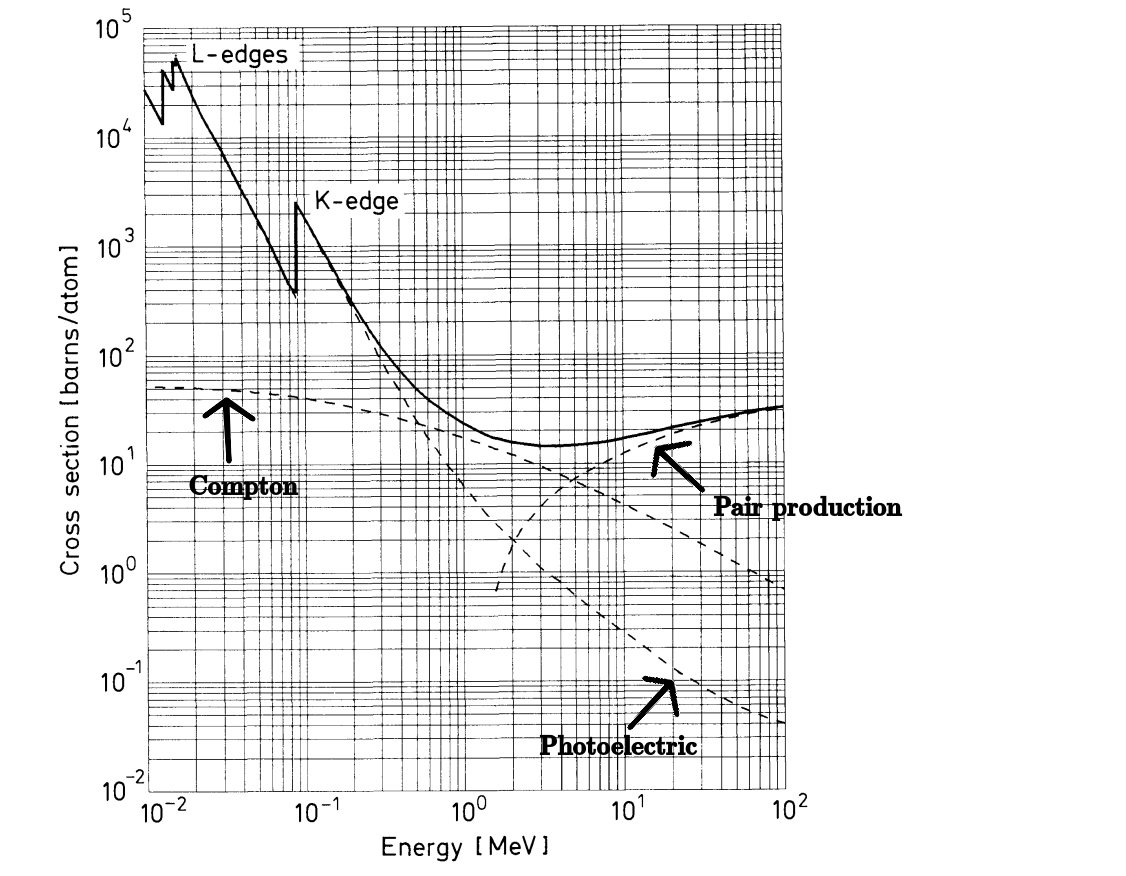
\includegraphics[scale=0.6, angle = 0]{./pictures/totalCross}
 \caption{Exapmpe of total absorption cross section for high-energy photons for lead. Taken and modified from \cite{Leo1987-wy}.}
 \label{cross}
 
\end{figure}
 


\subsubsection{Photoelectric effect}
The photon is absorbed by electron from atomic shell. The electron is ejected and acquires the kinetic energy given by well-known equation:
 \begin{equation}
 E = hf - E_{b},
 \end{equation}
where $f$ is the photon frequency and $E_{b}$ is the binding energy.
 
The Photoelectric effect can be observed only on electron bounded in atomic shell, due to the fact, that the nuclei can absorb the photon's momentum. The cross section usually falls with energy and can have characteristic peaks from K,L,M transitions.

\par

The photoelectric effect plays a key role when it comes to the detection of gamma photons.

\subsubsection{Compton scattering}
Compton scattering is an effect, which is mainly observed on free electrons. It needs to be said, that the electrons in material are usually bounded, however, if the photon energy is much higher than the binding energy, the electron can be considered as free.
\par
This effect causes, that the photon loses only a part of its energy and changes its direction. The energy is transferred to an electron accordingly to the laws of energy and momentum conservation and can be described by following relation:

\begin{equation}
E_{\textrm{e}} = E_1 - E_2 = E_1 (1- \frac{1}{1+\frac{E_1}{m_{\textrm{e}}c^2}(1 - \cos{\theta})})
\end{equation}


\par
Where $E_{\textrm{e}}$ - energy transferred to an electron, $E_1$ - initial photon energy, $E_2$ - scattered photon energy, $m_{\textrm{e}}$ - the electron mass and $\theta$ - angle of scattering. This equation can be used to calculate the positions of Compton edges in energy spectra by plugging the angle of maximum energy transfer ($\theta = 180^\circ$).


\subsubsection{Pair production}
At much higher energies, the photon can be converted into electron-positron pair. This effect happens near the nucleus, which absorbs a part of the original photon momentum.
\par
The pair production along with electron bremsstrahlung radiation  are key effects for electron-photon shower development. If the created electron/positron has sufficient energy, it emits bremsstrahlung photons. These bremsstrahlung photons can again interact via the pair production, and thus creating new electrons again. This process of shower development continues until the energy of electron/positron pairs drops under the energy, which is required to produce bremsstrahlung radiation. At lower energies, the electrons lose more of their energy by the atomic collisions rather than by bremsstrahlung.
\par
Negative effects arising from this type of interaction like creation of single and double escape peaks or annihilation peaks in spectra will not be observed, because for low-energy gammas the cross-section is very small. That means that for the purposes of this thesis, this interaction effect could be neglected.   


\subsection{Characteristic energy spectra}
Every gamma source emits its characteristic photons with certain probabilities. However, before these photons are captured by detector, many effects can occur in environment or inside the detector - photons can interact various materials without detection purpose such as shielding, spectrum can be altered by 
noise events in detector etc.
\par
Inside detector the low-energy spectra can be affected by:
\begin{itemize}
\item X-ray escape peaks - If the photo-effect occurs on atomic energy levels, the characteristic X-ray of the detector material is emitted. The escape peak has the energy of captured photon minus the energy of escaped gamma ray.
\item Compton continuum with edge - the photon interacts inside detector by Compton scattering, scattered photon leaves the detector.

\end{itemize}

In environment the low-energy spectra can be affected by:
\begin{itemize}
\item Characteristic X-rays - radiation induced fluorescence usually from the shielding material (Pb).
\item Backscatter peak - Compton scattering which occurred over a large angle.
\end{itemize}


For Mössbauer spectroscopy the $^{57}$Co is usually used with gamma spectra shown below:


% %%%%%%%%%%%%%%%%%%%%%%%% End of file %%%%%%%%%%%%%%%%%%%%%%%%

% -----------------------------------------------
% Vlastní text práce (kapitoly práce)
% -----------------------------------------------

% -----------------------------------------------
\chapter{Gamma rays detection}
% -----------------------------------------------


% -----------------------------------------------
\section{Properties and parameters of detectors}
% -----------------------------------------------
The main parameters which are crucial for purposes of Mössbauer are detection efficiency and energy resolution at low gamma energies.
\par
Nowadays three main types of detectors are employed on the field of nuclear physics - gas, scintillation and semiconductor.
The Mössbauer spectrometer setups in laboratories of KEF are usually based on gas or scintillation detectors.


\subsection{Gas proportional detectors}
The gas detectors are usually tubes with electrodes filled with a special gas mixture. The incoming particle ionizes the gas, creating free ions and electrons.  According to the applied voltage, the gaseous detector can be operated in proportional regime, which is characterized by additional multiplication of charge carriers and thus, the signal can be amplified. The advantage of gaseous detectors is that they offer good energy resolution, but on the other hand their detection efficiency is low mainly due to the fact, that the gas density is small. Count rates are also affected by the long duration of the ionization effect. For operation they require high voltages (usually over 1000 V) and in case of flow counters they also require pressure cylinders along with other heavy equipment. 

\begin{figure}[H]
 \centering
 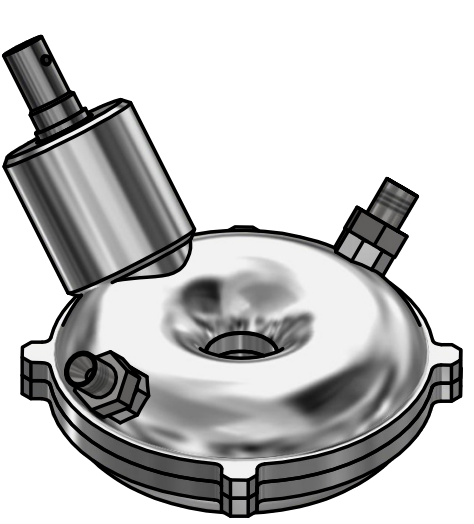
\includegraphics[scale=0.55, angle = 0]{./pictures/GASdet.png}
 \caption{Toroidal proportional gas flow counter used in MS spectrometer \cite{Optimized}.}
 \label{toroid}
 
\end{figure}


\subsection{Scintillation detectors}
By scintillation detector is usually meant a scintillation crystal coupled with a photomultiplier tube (PMT). The first conversion happens inside the scintillation crystal, where the incoming particle generates number of photons linearly dependent on its energy. These photons are captured by PMT's photo-cathode, where are they converted into electrons, and then multiplied on PMT's dynodes. This amplification requires high voltages around $1000 - 2000$ V. The internal amplification inside PMT can be around $10^6$.
\par
The detection efficiency is very high and due to the short duration of excitation effects, they can be used at high count rates.
\par
However, their energy resolution is much worse than in case of gases and semiconductors. The gamma spectra obtained this way usually have distorted wide peaks, which negatively affects Mössbauer spectrometry. The PMTs also cannot be employed inside the magnetic fields. 


\begin{figure}[H]
 \centering
 
\includegraphics[scale=0.35, angle = 0]{./pictures/NoPicture.jpg}
 \caption{Scintilator crystal coupled with PMT \cite{•}.}
 \label{PMT}
 
\end{figure}


\subsection{Detectors based on semiconductors}
The semiconductors offer the best energy resolution and a very good efficiency, however, they are usually expensive.

\par
The one problem with semiconductor detector is that there is no internal amplification, so the signals coming out of the detectors have to be strongly amplified by electronics.
\par
The semiconductors are small and compact. They also don't require high voltage sources and heavy pressure cylinders. These facts are crucial if it comes to making more compact Mössbauer spectrometers. The Mössbauer spectrometer MIMOS II \cite{https://doi.org/10.1029/2003JE002138} based on 4 Si PIN diodes was a part of two rowers Spirit and Opportunity and their mission on Mars. 




% %%%%%%%%%%%%%%%%%%%%%%%% End of file %%%%%%%%%%%%%%%%%%%%%%%%

% -----------------------------------------------
% Vlastní text práce (kapitoly práce)
% -----------------------------------------------

% -----------------------------------------------
\chapter{Semiconductor detectors with p-n junction}
% -----------------------------------------------
The semiconductor structures has unique properties, which make them usable not only for a particle/photon detection. There are many types of semiconductor detectors - conventional detectors of light intensity with spectral range from infrared to UV - photoresistors and photodiodes, low intensities and single photons detectors - avalanche photodiodes (APDs), for imagining - CCD and CMOS cameras, x-ray, gamma and other particles rates and energy detectors - special photodiodes, for particle position and energy measurements - matrix drift and strip detectors. The essential role for gamma spectroscopy have the p-n junction detectors - detection diodes capable of capturing gamma photons with sufficient energy resolution and efficiency.

\par
To detect Mössbauer 14.4 keV gammas our primary choice are the Si PIN diodes for direct detection due to the guaranteed high detection efficiency under 25 keV. 

\section{The Structure of semiconductor}
Since we are not dealing with single atoms characterized by the well-known discrete energy levels, but with solid crystals, there is another  model describing the energy levels - the band structure. The energy levels are very close each other that they nearly form a continuum. This different behaviour is a result of a periodical potential inside the crystal lattice. However, the electron energy $E_{n}$ is not the only quantum number describing the behaviour of electrons inside the periodical potential. By solving Schrödinger equation with the help of so-called Bloch's theorem, we come to a conclusion that the second important quantum number is the wave vector $\vec{k}$. These two quantum numbers are bounded together by dispersion relations $E = E(\vec{k})$, which is characteristic for every crystal and may play role when it comes to transitions of electrons between bands.

\subsection{Band structure}
The basic difference between conductors, insulators and semiconductors is the valence and conduction band structure. In case of conductors, the valence band overlaps the conduction band. The electrons in conduction band can move nearly freely throughout the crystal. For insulators, there is no overlap, and the energy band gap $E_{\textrm{g}}$ between the two bands is so high, that it makes any transitions of electrons nearly impossible. However in case of  semiconductors, the $E_{\textrm{g}}$ is small enough to allow the electron jump into the conduction band and leaving the hole in valence band after receiving a sufficient amount of energy - in form of thermal energy $E_{\textrm{T}} = kT$, energy in static electric field $E_{\textrm{s}} = -e\phi$ or as a photon with energy quantum $E_{\textrm{photon}} = \hbar \omega$. The last one is the most important, because it allows us to use the semiconductors as detectors. Both the electron and hole participates on conduction, but they have to be treated as quasiparticles with their specific masses and mobilities.


\subsection{Occupation of states}
The occupation probability of states in band structure is given by Fermi-Dirac distribution since the electrons are the Fermions with the exclusion rules. 
\par
The possible occupied state where occupation probability drops below 50 $\%$ is called the Fermi level with Fermi energy $E_{\textrm{F}}$. 
For ideal pure semiconductor at $T=0$ K, the $E_{\textrm{F}}$ lies in the middle of the band gap. With increasing temperature, in most materials the Fermi-level moves upper towards the conduction band.

\subsection{Semiconductor Crystals}
The semiconductor materials have usually form of a crystal of diamond structure (two FCC lattices bounded together.) with the lattice atoms bounded by a covalent bond. However in real crystals there are also defects and impurities which may alter the functionality. The impurities can be added on purpose to enhance the properties we seek in procedure called doping. 
\par
The suitable materials for construction of ionizing radiation detectors are Ge - very good energy resolution, requires cooling, Si - great efficiency under 25 keV, easier fabrication since many other semiconductor devices are being made of Si and CdTe - used in wide-spectre X-Ray and Gamma Ray Detectors.
\par
The fabrication of semiconductors for purposes of detection includes many complicated processes, because the detector requirements on crystal purity are very high.

\subsection{Direct and indirect semiconductors}
 
The shape of dispersion relations $E(\vec{k})$ divides the semiconductors into two categories - direct and indirect semiconductors. For direct semiconductors the minimum in conduction band and maximum in valence band have the same $\vec{k}$, so the transition can occur after the $E_{\textrm{g}}$ is supplied. In case of indirect the minimum and maximum have different $\vec{k}$. To make transition, additional momentum has to be server (for example by phonons) or the supplied energy must be much larger to allow transition to the higher state. %with the same $\vec{k}$.  
The Si crystal is an indirect semiconductor.


 
\section{The p–n junction}
The intrinsic semiconductors have only a little field of applications. We can alter the behaviour by adding a specific impurities and create an extrinsic semiconductor. The Si atom has 4 valence electron which form a covalent bond with other Si atoms. If Si atom is replaced with atom with 5 valence electrons, one of them will have a very weak bond.
By doping the intrinsic semiconductor with these atoms we create the $n$-type with additional electrons, which are nearly localized in conduction band. However, the crystal as whole stays neutral. Similar way doping by atoms with only 3 valence electrons, there will be holes in valence band, which can participate on conduction - the $p$-type.
In band structure These atoms create energy levels in band structure, but in room temperatures, they are all mostly ionized and participate on conduction. The full theoretical treatment of doping is very complex, considers many other quantum and statistical physics aspects, and have no use for the purposes of this thesis. 

\par
The special effects will arise when $p$-type and and $n$-type are bound together. The holes from $p$-type and electrons from $n$-type will start to diffuse to the other region. However, this movement alter the charge density, which leads to creation of built-in voltage which in the end cancels the diffusion. This creates the depleted region, where are no free charge carriers. 
\par
Another theoretical view is that the electrons will rearrange, because the Fermi-level has to be same throughout the crystal, while the Fermi-level for stand-alone $p$-type is nearer to the valence band and for $n$-type is nearer to the conduction band. The potential created this way equalizes the different Fermi levels. 

\par
The p-n junction can be connected to source voltage in two ways. The $p$ layer on plus - the source voltage (refereed as bias) reduces the size of depleted layer until it completely vanishes (bias goes against built-in voltage) and the p-n junction becomes conductive - forward direction or in reverse direction - $p$ layer on minus (bias goes with built-in voltage), the size of depletion layer increases.


\par
The p-n junction has many unique properties, which are commonly used in form of classical diodes. However, it is also crucial for the detection since the free charge carriers (if somehow created) in depleted layer are pushed towards electrodes by electric field and form a photocurrent.

\par
For the purposes of design in electronic circuits, the detectors are usually modelled as classical p-n diodes, which are connected to the source of the bias voltage in reverse direction. In case of detection, the detector can be also modelled as a current source.


\par
The voltage across the depleted layer could be modelled as a simple plate capacitor. The capacitance of p-n junction plays a significant role - it alters the dynamical parameters of the detection circuits - it can alter the rising edges of pulses, alter the entire frequency spectra, increase/decrease the SNR. By varying the source voltage we vary this capacitance too.

\par
There is also one more problem with the diffusion of electron and holes which has to be considered. It is the diffusion of charge carriers from the $p$ and $n$ layers to the metal ohmic contacts on electrodes, which can form an unwanted electric field and a potential barrier across the contact. To prevent this from happening, the regions around the ohmic contacts are highly doped to reduce the potential barrier size. 


\section{Detection mechanism}

\par
If we want to detect a particle or photon, is has to interact with the detector material - in semiconductor the creation of electron-hole pairs is observed. This could be achieved by interaction mechanisms described in previous chapters, which differ for every type of particle and energy. 

\par
The main of purpose of semiconductor as a detector, is to perform a linear conversion of the particle/photon energy into the free charge carriers - electrons in conduction band and holes in valence band. The average energy needed to create a single electron-hole pair is usually a fix constant - in Si it is $\epsilon = 3.6$ eV \cite{Lutz_2007}. Since the Si is an indirect semiconductor, this value is not equal to gap energy, which is lower ($E_{\textrm{g}} = 1.12$ eV). In case of low-energy gamma the two main mechanisms which take place in producing the charge carriers are photo-effect and Compton scattering. 

\par
The gamma photon striking the detector firstly interacts with a single electron. If the photo-effect takes its place, the primary electron with energy much higher than the thermal excitation will ionize the electrons from all over the valence band pushing them into higher states from conduction band. These Electrons in conduction band de-excite themselves into lower states of conduction band and the holes redistribute themselves to the upper states in valence band. This redistribution process releases energy again which leads to the cascade of further excitations and interactions, which produce many electron-hole pairs - the charge cloud. Number of generated electron-hole pairs $n$ is simply given by relation:


\begin{equation}
n = \frac{E_{\textrm{gamma}}}{\epsilon}.
\end{equation}

\par
In case of compton, the scattered photon may escape the detector without any other interaction taking the rest of its energy out of the detector. This results into energy distortion. The compton without any other interaction (compton again or photoeffect) is typical for thin detectors since there is insufficient thickness to stop the scattered photon again. In detected gamma energy spectrum this leads into compton continuum with the compton edge,which devaluates the spectra.

\par
An ideal very thick detector could solve this problem, because every possible interaction and all the following sub-interactions will happen inside the detector and will result into electron-hole generation. The detector of this kind would have only the full energy peaks without any other unwanted counts. However, construction of such detector is impossible due to the many technical and manufacturing problems arising with increasing dimensions. 

\par
In case of p-n junction the created charge carriers in depleted layer are pushed towards electrodes by internal electric field. The  electronics accumulates the charge and converts it into the voltage pulse signal, which is then analysed to extract the energy information. Since the depleted layer is the only part where the detection can occur, its obvious that for detector purposes it should be large as possible. 
\par
To achieve the greater dimensions of the detection part, the p-n junction can be upgraded to p-i-n junction, which contain additional intrinsic layer between $p$ and $n$ part, which work as fix size depleted layer. The detectors with p-i-n junction are referred as PIN diodes. The additional intrinsic layer also decreases the capacitance and increases the time needed for charge carriers to exit the detection part.

\section{Main noise sources and resolution limitations}
The detection efficiency and the energy resolution are strongly dependent on noise which alters the signal. While some negative effects are caused by outer conditions such as temperature or by noise in electronics, some originate strictly from semiconductor material properties and only chance to minimize them is during the crystal's preparation.

\subsection{Fano noise}

The physical effect inside the semiconductor itself which limits the measured energy resolution is the fact that not all of the particle's energy is transformed into charge carriers. Some fraction of energy can be consumed to induce lattice vibrations (phonons). Statistically the relative resolution can be described by following equation:


\begin{equation}
\frac{\Delta E}{E} = 2.35\sqrt{\frac{F\epsilon}{E}},
\end{equation}
where $E$ is incoming particle's energy, $\epsilon$ is the average energy needed for the single pair creation and $F$ is a Fano Factor. Fano Factor is a special statistical constant which describes the dispersion in counting process. For Poisson distribution the $F$ is 1. If we consider the case of 14.4 keV gamma inside Si ($\epsilon = 3.6$ eV, $F = 0.12$), the $\frac{\Delta E}{E}$ is equal to 1.3 $\%$ and $\Delta E$ is 185.4 eV.
\par
This resolution is sometimes called intrinsic, because the real resolution is much worse. This model does not consider other sources of noise coming from the amplification in electronics, dark currents e.g. 




\subsection{Thermal noise}

It was mentioned that the electrons can be also excited by thermal fluctuations. However, since the many of detector's materials are indirect semiconductors, the thermal excitations are carried through the intermediate states inside the band gap. These states have the origin in imperfections and impurities inside the crystal lattice. The electrons and holes generated this way can join the charge cloud generated by detected particle and decrease the SNR. This phenomenon is usually called dark current.

\par
The thermal fluctuations are much more significant for materials which require less energy to excite the electrons to the conduction band such as Ge. These detectors always have to be operated at low temperatures. Even the room temperature can lead up to the breakdown and destruction of a detector. For Si, the valence and conduction band are more distant. so the thermal fluctuations are not so critical.
\par
However the applied bias voltage in reverse direction usually also increases the dark current.


\subsection{Recombination and trapping}
The effect which goes against the successful collection of charge carriers and thus affects the detection efficiency and the energy resolution is recombination. In pure crystals, the electron can recombine with hole only when they have the same $\vec{k}$. However, inside real crystals there exists impurities, which allow carriers to recombine - recombination centres. The charge collection must take much less time than it takes the carriers to recombine. 
\par
Another effect caused by the very same impurities is trapping. The trapping centres capture electron or hole and release it after certain time. This effect alter the signal pulses and can decrease maximum possible counting rate.
\par
Energy levels near the centre of band gap are primary responsible for recombination and trapping, which means that the impurities causing this are not the impurities which were added in doping, because these have their additional energy levels near the bands. 


\section{Structure and parameters of Si PIN detector}
One of the most important parameter is the size of the photosensitive area, which has to be large as possible for effective collection of radiation. This area has to be treated with extreme caution since every damage, adsorption of impurities or dew condensation due to the high environmental humidity reduces the active photosensitive area.

\par
Its obvious that for the interactions inside the detector the most crucial layer dimensions are those, which are parallel to the direction of incident radiation - the thicknesses of P and I regions.
The dead region (P) has to be thin as possible to reduce probability that the particle interacts in place where the generated charge cloud would nearly immediately recombine. The active depleted (I) layer has to be thick enough to make all the interactions happen inside itself. The schematic of PIN diode can be seen on fig. \ref{SiPIN}.


\begin{figure}[H]
 \centering
 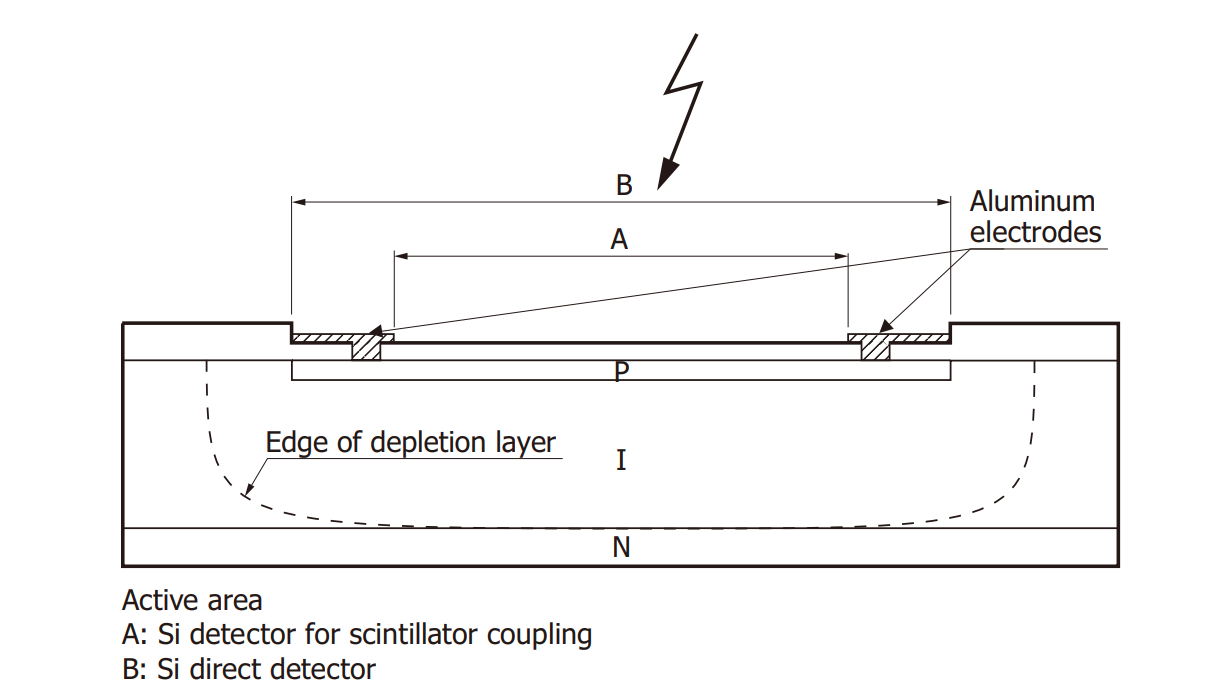
\includegraphics[scale=0.35, angle = 0]{./pictures/SiPINScheme.png}
 \caption{Cross section of Si detector for scintillator coupling and Si direct detector \cite{SiPINdirect}.}
 \label{SiPIN}
 
\end{figure}



\section{Available Si PIN detectors}
For testing we have chosen one professional Hamamatsu S14605 PIN diode and two commercial PIN diodes: OPF420 - originally designed to be used in optical fibres, BPW34 - visible and near infrared radiation detector.  



\subsection{Hamamatsu S14605}
The professional S14605 is designed to be used as a direct radiation detector. It offers a very large photosensitive area and a low capacitance.

Parameters \cite{datS14605}:
\begin{itemize}
\item Maximum reverse voltage $U_\textrm{R}$: 150 V
\item Photosensitive area: 81 mm$^2$
\item Capacitance: 25 pF at $U_\textrm{R} = 100$ V
\item Dark current: 8 nA at $U_\textrm{R} = 100$ V
\item Depletion layer: 0.5 mm
\item Cost: 5000 CZK
\end{itemize}

\begin{figure}[H]
 \centering
 
\includegraphics[scale=0.35, angle = 0]{./pictures/NoPicture.jpg}
 \caption{Hamamatsu S14605.}
 \label{S14605}
 
\end{figure}

\subsection{OPF430}
OPF430 is originally ment to be a low-cost detector for fiber optic applications. However, there were publications \cite{RAMIREZJIMENEZ2003577}, which described the possibility of using similar diode OPF420 in low-energy gamma spectroscopic chains as a low-cost detector.

Parameters \cite{datOPF430}:
\begin{itemize}
\item Maximum reverse voltage $U_\textrm{R}$: 100 V
\item Photosensitive area: not specified, small
\item Capacitance: 1.5  pF at $U_\textrm{R} = 5$ V
\item Dark current: 0.1 nA at $U_\textrm{R} = 5$ V
\item Depletion layer: not specified
\item Cost: 340 CZK
\end{itemize}

\begin{figure}[H]
 \centering
 
\includegraphics[scale=0.35, angle = 0]{./pictures/NoPicture.jpg}
 \caption{OPF430.}
 \label{OPF430}
 
\end{figure}

\subsection{BPW34}
BPW34 is a very low cost radiation detector. There were manuals \cite{betaBPW} how to use BPW34 as a beta particle detector, and since it is a Si PIN diode, it worths a try and test it for our gamma detection purposes.



Parameters \cite{datBPW34}:
\begin{itemize}
\item Maximum reverse voltage $U_\textrm{R}$: 32 V
\item Photosensitive area: 7.5 mm$^2$
\item Capacitance: 25 pF at $U_\textrm{R} = 3$ V
\item Dark current: 2 nA at $U_\textrm{R} = 10$ V
\item Depletion layer: not specified
\item Cost: 30 CZK
\end{itemize}

\begin{figure}[H]
 \centering
 
\includegraphics[scale=0.35, angle = 0]{./pictures/NoPicture.jpg}
 \caption{BPW34.}
 \label{BPW34}
 
\end{figure}

% %%%%%%%%%%%%%%%%%%%%%%%% End of file %%%%%%%%%%%%%%%%%%%%%%%%


% -----------------------------------------------
% Vlastní text práce (kapitoly práce)
% -----------------------------------------------

% -----------------------------------------------
\chapter{Mössbauer effect and spectroscopy}
% -----------------------------------------------
Mössbauer effect is a physical effect, which can under certain circumstances occur on atomic nuclei. It consists of recoilless resonance emission/absorption of gamma photons by nuclei of source/absorber with discrete nuclear energy levels. This effect has a special application on the field of material research - the Mössbauer spectroscopy, which is a nuclear experimental technique and a special type of gamma spectroscopy, which uses the appropriate nuclei in studied sample as sonds of local electric and magnetic fields. 

\par
This technique is capable of providing many unique information in material research, geology, chemistry and biology - study of phase and chemical composition of solid materials such as steel, study of local magnetic fields and spin states, in-situ measurements of phase transitions. The main disadvantage of this technique is the fact that there is not an appropriate radiation source for many isotopes. The mayor significance has iron and its isotope $^{57}$Fe with possible radiation source $^{57}$Co (which decays into an excited state of $^{57}$Fe with half-life 271.81 days \cite{co57}), which allows the Mössbauer spectroscopy to be employed on many fields, including the steel industry.

% -----------------------------------------------
\section{Physical concept}

\subsection{Resonace emission and absorption}
In previous chapters was mentioned, that the atomic nuclei are quantum systems with discrete energy levels (analogous to the energy levels of electron shell), thus upon deexcitation or excitation they emit/absorb gamma photon with energy $E_0$ equal to the difference between the levels. For the free, stationary nucleus, the emitted/absorbed energy spectra follow the shape of Lorentzian curve. 

\par
However, these emitted/absorbed energy spectra may be altered - due to the  momentum conservation law, some part of the gamma photon energy is transferred to the  kinetic energy of nucleus, crystal as whole body or is transformed into lattice vibrations (phonons). 
%Due to this fact, the emission and absorption energy spectra may be different and without any overlaps, which prevents the resonance effects from happening.
In the case of free, stationary nuclei, momentum and energy transfers are so high, that the emission and absorption spectra are shifted to different directions by large energetic values, which makes the resonance absorption impossible to observe. However, the nucleus bounded into the crystal lattice is a different case - the crystal as whole body will absorb the momentum. If we consider, that the entire crystal has much larger mass than the nucleus, the energy transfer into crystal's kinetic energy will be very small - the gamma photon energy remains nearly unaltered. Thus this can be considered as recoilless emission/absorption and the energy spectra have overlap, which makes the resonance absorption (Mössbauer effect) observable \cite{moss}.
\par
It also worth mentioning, that there is also a third case - the free nuclei in thermal motion. The velocity of nuclei is guided by Maxwell's statistics and the spectra become widened by Gaussian shape. At higher temperatures, this effect may result into spectra overlap and makes the resonance absorption observable. However, this technique is not much developed yet and has only a small field of application.

\subsection{Interaction of nuclei with local fields}

The nucleus bound inside the lattice surrounded by electrons arranged according to the chemical bonds has perturbed energy levels, which is due to the interaction of nucleus with local electric and magnetic fields -  what results into the fact, that every phase or chemical constitution has its own nuclear emission/absorption spectrum - Mössbauer spectrum. The quantum physics has very-well known computation techniques to describe these variations in energy spectra - the perturbation theory,

\par
The main properties of nucleus which induces the interactions with local electric and magnetic fields are: atomic number $Z$, quadrupole momentum $Q$ and its spin $I$ along with its projections. For spectroscopy there are three main interaction:

\begin{itemize}
\item Electric monopole interaction - the interaction between the protons of nucleus and the s-electrons (which have non-zero probability of being found inside nucleus). It results into isomer shift of energy levels $\delta = E_M - E_0$. The $\delta$ has to be defined with respect to some fixed energy level, for example to the level of the used source. This type of MS spectra is usually referred as a singlet. 
\item Electric quadrupole interaction - the inhomogeneous electric field inside nucleus interacts the quadrupole momentum $Q$ of the nuclei. It results into energy variations with respect to the square of magnetic quantum number $E_Q \sim m^{2}$- the states which allows different values of $|m|$ are splitted into sub-states.

\item Magnetic dipole interaction - the spin $I$ is tied up with magnetic momentum via relation $\mu = \gamma I$, where $\gamma$ is a gyromagnetic ratio. This magnetic momentum interacts with magnetic fields inside nucleus and results into nuclear Zeeman effects - the splitting of the states with respect to possible values of magnetic quantum number $m$. The main difference from the quadrupole interaction is that the spin orientation also matters. The magnetic dipole interaction has a significant role when it comes to study the magnetic properties of materials.
\end{itemize}

Each of these effects can occur separately or simultaneously with the others.


% -----------------------------------------------



\section{Mössbauer spectroscopy}
There are several techniques how to obtain the spectra. In laboratories there are dominant the setups employing transmission or backscattering geometry with sample as an absorber and with the doppler modulation of the gamma photons energy. The transmitted photons or other products developed upon deexcitation are detected by appropriate detector with electronics to accumulate the energy spectra. The energy of gamma photons is varied by the doppler effect - the source is attached to the doppler modulator (transducer), and by the relative velocity of source and absorber the energy of gamma photons is slightly changed.
\par
For transmission geometry the key concept of measurement is that if we irradiate the sample as an absorber gradually by continuous spectrum of gamma rays with energy around the resonance energy $E_0$ ("energy scanning" by the doppler modulator), the gamma photons with energy equal to one of the possible transitions (resonant energies) are absorbed with certain probability. 
%Gamma photons with different energies are due to the low cross section of previously discussed matter interactions mostly transmitted.
The detector is situated behind the absorber and simultaneously measures the number of gamma counts at defined energy step. The minimal counts are measured around the resonant energy. The transmission geometry Mössbauer spectra can be seen on picture \ref{transspec}.

\par
The concept of backscattering geometry is similar in many ways, but the main difference is the detection of the deexcitation products. The sample's nuclei are excited by appropriate gamma photons and in short time, they decay back into the original state with some effects following - reemission of the "original" gamma photons in random direction, emission of electrons from the shell (ejected by deexcitation energy quanta, also called conversion electrons) followed by characteristic RTG or possibly by auger electrons. The detection of electrons and RTG instead of gamma photons have many advantages and disadvantages and for certain application, the usage of backscattering geometry could be more appropriate. For example, the detection of conversion electrons could handle the surface characterization of the sample due to the lesser transmittance of electrons when comparing to gamma photons.


\par
There are also different setups - irradiation by synchrotron radiation (which can produce continuous gamma spectra with high iluminance), using the sample as an source etc.



\section{$^{57}$Fe spectroscopy}

One of the isotopes, on which we are capable to observe a Mössbauer effect is $^{57}$Fe. As a source is used $^{57}$Co, which decays into second excited state of $^{57}$Fe by electron capture. The new $^{57}$Fe nuclei can deexcite itself by two ways (see fig. \ref{Fe57scheme}) - by direct deexcitation onto ground state by emitting 136.5 keV photon or by deexcitation onto the first excited state by emitting 122.1 keV photon and after short lifetime emits 14.4 keV photons (or other possible conversion products) when falling into ground state. The $^{57}$Fe spectroscopy in transmission geometry is based on detection of the 14.4 keV gamma photons. This thesis is mainly devoted to the application of semiconductor detectors for the detection of these 14.4 keV gamma photons. The $^{57}$Fe spectroscopy can also be performed in backscattering geometry by the detection of the conversion electrons or RTG photons with energies around 6.4 keV.

\begin{figure}[H]
 \centering
 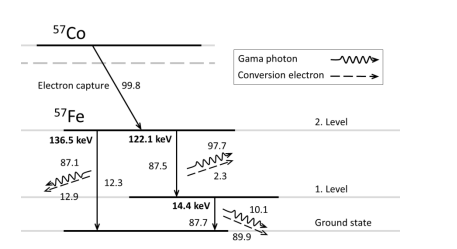
\includegraphics[scale=0.75, angle = 0]{./pictures/Fe57}
 \caption{Decay scheme of $^{57}$Co, taken from \cite{NOVAK2016thesis}.}
 \label{Fe57scheme}
 
\end{figure}


The entire spectrometric setup consist of several parts:
\begin{itemize}

\item Source of 14.4 keV gamma - $^{57}$Co radioctive nuclei built-in crystal lattice (mostly in a rhodium matrice). The source is attached to the transducer.
\item Transducer for doppler modulation. It mostly consists of two coils surrounded by permanent magnets - one for setting the velocity of the source and second for the velocity measurement. The system is driven by PID or MPC controller for precise velocity and energy control. The velocity can be either constant or with constant/varying acceleration.

\begin{figure}[H]
 \centering
 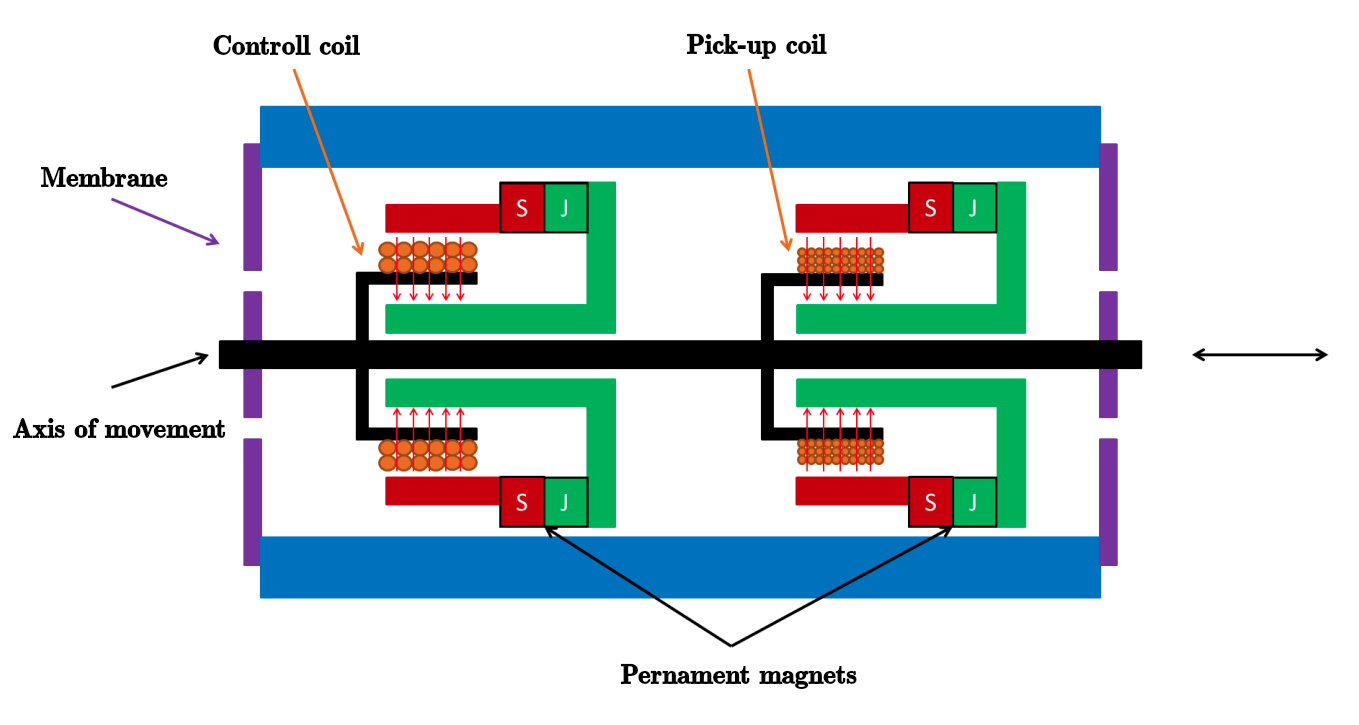
\includegraphics[scale=0.4, angle = 0]{./pictures/transducer}
 \caption{Transducer, taken from \cite{STEJSKAL2019thesis}.}
 \label{transducer}
 
\end{figure}

\item detector of transmitted/backscattered gamma radiation, conversion electrons or RTG along with readout and evaluation electronics including amplifiers, SCA's, MCA's etc. It is also necessary to consider, that the already mentioned conventional detectors have not sufficient energy resolution to distinguish the energy of perturbed states. Because of that, the count rates are synchronised with the velocity signal (actual modulated energy), which is used to address the channels for spectra accumulation. 
%The other approach is to address the channels by precise timing.

\end{itemize}
The functional diagram can be seen on fig. \ref{spectrometric setup}.

\par
It is also necessary to consider, that the $^{57}$Fe isotope have relative abundance only $2.21 \%$ \cite{compounds}. Although this fact, the spectra are still measured with very respectable precision and efficiency, which makes the Mössbauer spectroscopy very sensitive measurement method.

\section{MS spectra quality parameters}
The MS spectra shape can be modelled by Lorentzian curves. The singlet spectra in transmission geometry can be modelled by a single Lorentzian curve in the following form:

\begin{equation}
\begin{aligned}
L(v) = -I\frac{(\frac{\Gamma}{2})^2}{(v - v_0)^2 + (\frac{\Gamma}{2})^2} + B
\end{aligned}
\label{lor}
\end{equation}

Where $I$ is the amplitude, the $\Gamma$ is the FWHM, and the $B$ is a background level. The Lorentzian in this form has the associated area $A$ equal to:

\begin{equation}
\begin{aligned}
A = \pi I \Gamma
\end{aligned}
\label{area}
\end{equation}

There are two properties of MS spectra which characterize its quality: SNR and the Effect $E_{\textrm{MS}}$. They can be calculated from spectra parameters by following equations:

\begin{equation}
\begin{aligned}
\textrm{SNR} = \frac{I}{\sqrt{B}}
\end{aligned}
\label{SNR}
\end{equation}

\begin{equation}
\begin{aligned}
E_{\textrm{MS}} = \frac{I}{B}
\end{aligned}
\label{effect}
\end{equation}



% %%%%%%%%%%%%%%%%%%%%%%%% End of file %%%%%%%%%%%%%%%%%%%%%%%%


% -----------------------------------------------
% Vlastní text práce (kapitoly práce)
% -----------------------------------------------

% -----------------------------------------------
\chapter{Electronics for signal readout and analysis}
% -----------------------------------------------
The signals coming out the detector has to be properly preamplified, amplified and shaped. This  task requires special analog circuits with properly designed layout. 
In our case, we use instruments, modules and parts from two companies - ORTEC and CREMAT. When designing the spectrometric measurement chain, we select components in order to achieve sufficient parameters for our application - energy resolution, low dead time to increase maximum possible counting rates e.g. 
\par
The task of realizing the spectrometric chain can be fulfilled in two ways. The first and more straightforward way is to build it from stand-alone robust instruments and modules. This can be more practical approach for testing of the detectors themselves since we are not forced to solve problems arising from badly designed electronic circuits. However, these modules are usually very expensive, measurement setups build this way are unnecessarily large and have worse noise parameters than electronic circuits specially tailored for the given application.
\par
The second possibility is to design printed circuit board (PCB) with required functionalities from electronic parts, However it requires many electronic engineering skills and additional time for development. The analog PCBs are very hard to design. The pros are that the final product can be very compact, and the electronic parts and PCB manufacturing is much cheaper. In this thesis, we apply both methods for the development.



\section{PIN detector connection and support electronics}
\subsection{Voltage source}
The PN and PIN detectors require voltage bias to reduce the capacitance.
These voltage sources don't have to be stiff since the detector's current consumption is very low.
\par
Gas and scintillation detectors usually require high voltage source (hundreds or thousands of volts). These high voltages are usually supplied by switching power supplies.
However, these supplies are usually very noisy and since the semiconductors can be operated at much lower voltages, there is no need for them. The better alternative is charge pump build of capacitors and diodes, which requires lower frequencies to operate.
\subsection{Shielding and grounding}

In case of sensitive analog signal circuits, the electromagnetic shielding is a very important part. Sensitive circuits have to be surrounded by a metallic material from all sides, which is also correctly connected to GND (principle of the Faraday cage), otherwise the proper functionality can not be guaranteed. The electromagnetic field from an outside source usually induces currents in the shielding material, and thus the special care has to be taken to prevent these induced currents from flowing through the signal routes. The figure \ref{shielding} shows the difference between correct and wrong connection of shielding.

\begin{figure}[H]
 \centering
 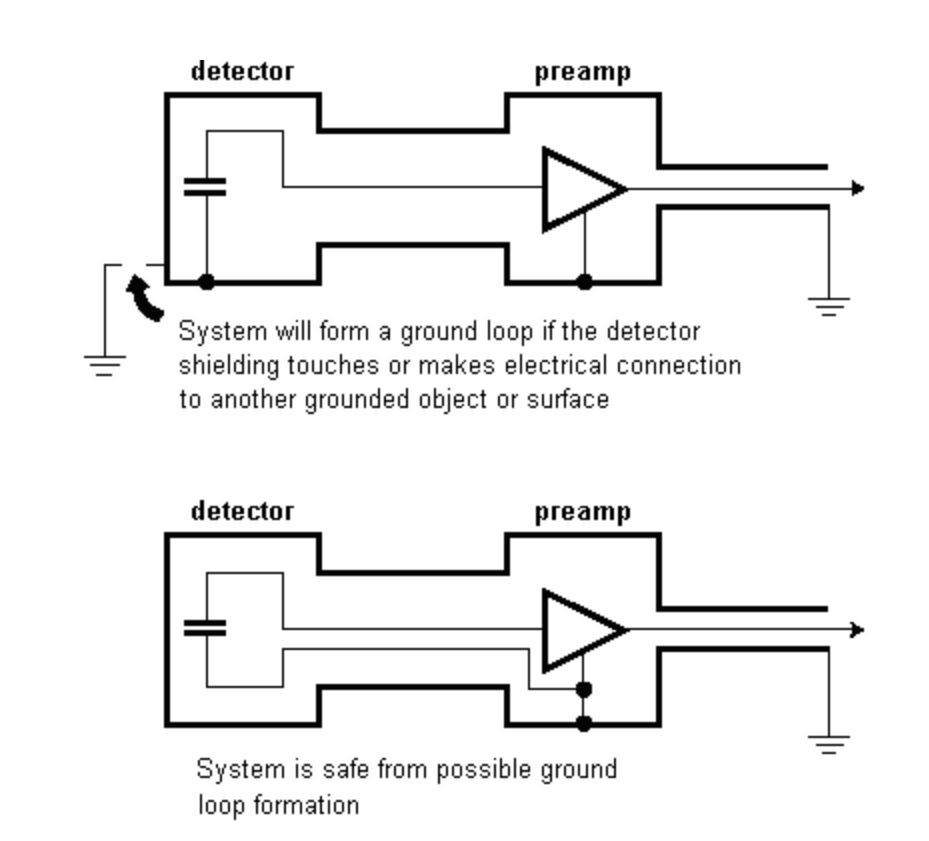
\includegraphics[scale=0.35, angle = 0]{./pictures/shielding.png}
 \caption{Schematic of wrong and correct connection of shielding \cite{appCSPnote}.}
 \label{shielding}
 
\end{figure}



\subsection{Cooling}
To reduce thermal noise and achieve better SNR it is necessary to cool the detector. The cooling can be achieved by various ways. In most setups, the appropriate solution can be provided by a peltier cooler. These setups with peltier are the easy to implement, however, their cooling efficiency is highly dependent on the ability to sink the heat from the hot side.

\section{Spectrometric chain}
The measurement chain for gamma spectroscopy is usually realized in following order - gamma detector, preamplifier, amplifier, multichannel analyser (MCA), microprocessor/computer.


\begin{figure}[H]
 \centering
 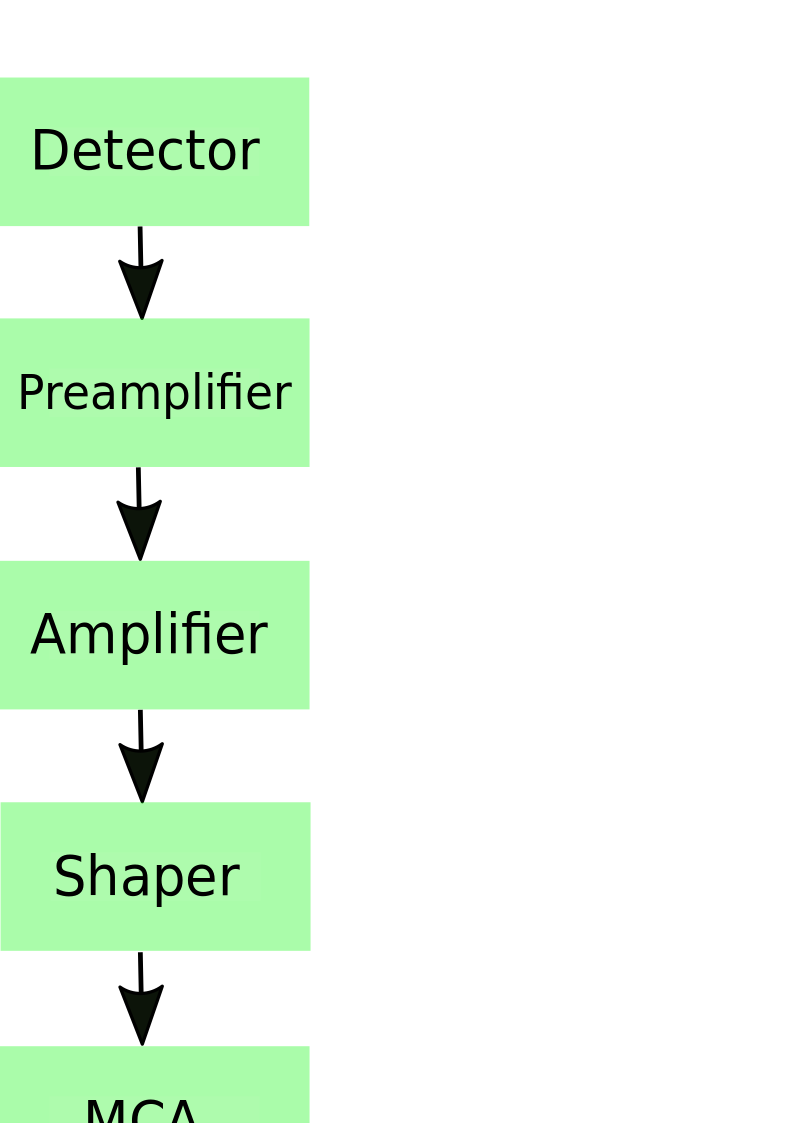
\includegraphics[scale=0.35, angle = 0]{./pictures/chain.png}
 \caption{Spectrometric chain.}
 \label{chain}
 
\end{figure}

\subsection{Pre-amplification}
The signal coming out of the PIN detector is weak, and it is also in form of charge (current pulse), so it is necessary to convert it into voltage pulse. For performing the charge-voltage conversion, one and the best solution is circuit called charge amplifier (also referred as a preamplifier). The principal functional scheme can be described by one opamp with a capacitor in feedback. The functionality is similar to $I/U$ transimpedance amplifier, but the charge amplifier works mainly as an integrator. In ideal case (opamp amplification $A >> 0$), the measured voltage per unit charge is approximately equal to:

\begin{equation}
\frac{dU}{dQ} = \frac{1}{C_{f}}.
\end{equation}


\begin{figure}[H]
 \centering
 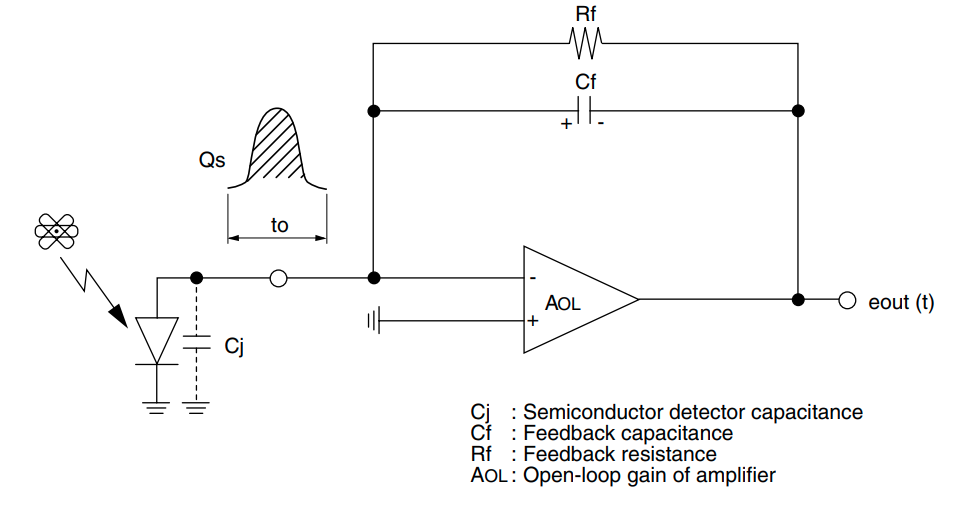
\includegraphics[scale=0.4, angle = 0]{./pictures/champlifier.png}
 \caption{Charge ampifier. $Qs$ is total charge of pulse and $to$ is the interval of charge generation inside the detector. Taken from \cite{charge}.}
 \label{trans}
 
\end{figure}



\par
In real circuit there is also a resistor parallel to the feedback capacitor. The feedback resistor slowly discharges the capacitor after a accumulation of charge, restoring the transimpedance amplifier to be ready to capture another pulse.

\begin{figure}[H]
 \centering
 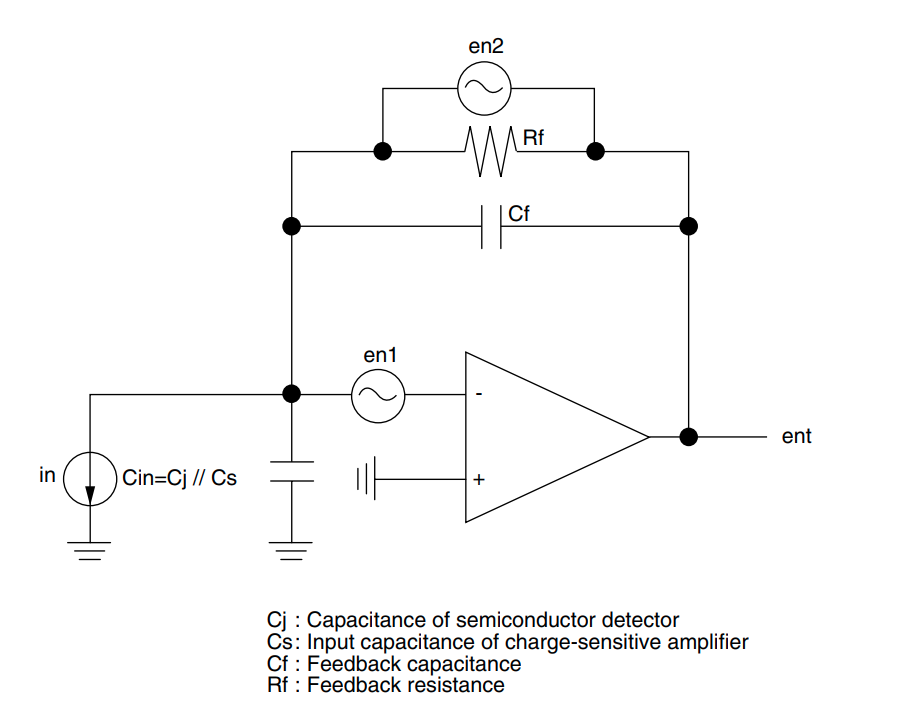
\includegraphics[scale=0.4, angle = 0]{./pictures/NoiseEquiv.png}
 \caption{Noise equivalent circuit for charge amplifier. Taken from \cite{charge}.}
 \label{trans}
 
\end{figure}


However, the functionality of charge amplifier is also negatively affected by an electronic noise, which depends on the values of the feedback resistance and capacitance and also on the internal parameters of the connected semiconductor detector and FET (field-effect transistor) inside the amplifier.

This electronic noise can be divided into three contributions, each described by euqations for noise voltages and currents \cite{charge}:

% on including the detector's capacitance $C_{\textrm{det}}$. Thermal noise dependency on $C_{\textrm{det}}$ of the first-stage FET transistor can be approximated by equation \cite{charge}:
\begin{itemize}

\item Thermal noise of first-stage FET:

\begin{equation}
en_1 = \sqrt{\frac{8}{3}\frac{kT}{gm}},
\end{equation}

where $k$ - Boltzmann constant, $T$ - absolute temperature and $gm$ - transconductance of FET. 

\item 

Shot noise caused by FET's gate current and detector's dark current:

\begin{equation}
in = \sqrt{2e(I_{\textrm{G}} + I_{\textrm{D}})},
\end{equation}

where $e$ - elementary charge, $I_{\textrm{G}}$ - gate leakage current of first-stage FET and $I_{\textrm{D}}$ - dark current of detector.



\item

Thermal noise caused by feedback resistance: 

\begin{equation}
en_2 = \sqrt{4KTR_{\textrm{f}}},
\end{equation}

where $R_{\textrm{f}}$ - the feedback resistance.

\end{itemize}


The square of total noise $ent^2(j \omega)$ is given by equation:


\begin{equation}
\begin{aligned}
ent^2(j \omega) = en_1^2 \cdot (1+\frac{C_{\textrm{in}}}{C_{\textrm{f}}})^2 + \{in^2 + (\frac{en_2}{R_{\textrm{f}}})^2 \}\frac{1}{(j \omega C_{\textrm{f}})^2},
\end{aligned}
\label{finalNoise}
\end{equation}

where the $C_{\textrm{f}}$ - the feedback capacitance and $C_{\textrm{in}}$ - the total input capacitance, resulting capacitance on the input of amplifier (there - parallel combination of detector's capacitance $C_{\textrm{j}}$ and amplifier's input capacitance $C_{\textrm{s}}$).   
\par
The first term in equation \ref{finalNoise} depends on the ration between the input capacitance $C_{\textrm{in}}$ and the feedback capacitance $C_{\textrm{f}}$ and thus the preamplifier's feedback capacitance has to be optimized in order to reduce the electronic noise.


\par
The charge sensitive preamplifiers modules usually also contain the second stage - common voltage amplifier. The internal scheme of CR-110-R2 charge amplifier made by Cremat Inc., which we use in the case of PCB design can be seen In the Fig. \ref{internal}.

\par

\begin{figure}[H]
 \centering
 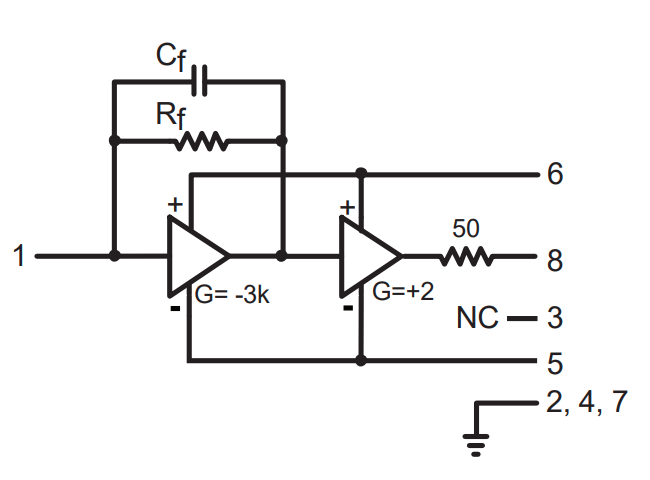
\includegraphics[scale=0.35, angle = 0]{./pictures/CRpreamp.png}
 \caption{Internal scheme of CR-110-R2 charge sensitive preamplifier \cite{cr110}.}
 \label{internal}
 
\end{figure}

The output voltage has the shape of exponential decay with amplitude defined by energy deposited into detector, short rise time (in orders of nanoseconds) and a longer decay constant (microseconds).


CR-110-R2 offers the conversion gain $G = 1.4$ V/pC, decay constant $\tau = 140$ $\mu$s CR-110-R2) and noise (FWHM) in silicon equal to 1.7 keV \cite{cr110}. It can be easily calculated, that for 14.4 keV photon, the output pulse has amplitude equal to $U_{A} = 0.8928$ mV. 
Note that the noise caused by the preamplifier is much larger than the intrinsic fano noise (FWHM = 185.4 eV).


\par
The modular version suitable for our application is ORTEC 142A charge preamplifier with $G = 1.016$ V/pC, $\tau = 500$ $\mu$s and noise in silicon equal to 1.6 keV \cite{ORTECpreamp}. Charge preamplifiers are usually very sensitive devices and can be very easily damaged by electrostatics. 

\par

Since the output of preamplifier is in order of millivolts, it has to be strongly amplified. Very fast and low noise amplifier consisting of multiple opamps is an appropriate solution of this problem.



\subsection{Shaping}

To perform the accurate energy discrimination, the pulse shape has to be altered from exponential decay shape by a shaping circuit. The shaping results into filtering the frequency band (reducing the noise) and also into shortening the long decay times of original exponential shapes. The shorter duration of pulses prevents the negative effect in which is one pulse superimposed onto another (pile-up effect).

\par
The Gaussian shape meets the sufficient parameters of SNR and duration \cite{Shapflify}. This type of shaping is usually achieved by several integration stages. The Cremat module CR-200-1us-R2.1 offers gaussian shaping with shaping time 1 $\mu$s \cite{cr200}. Its simplified internal schematic can be seen on fig.\ref{internal2}. 


\begin{figure}[H]
 \centering
 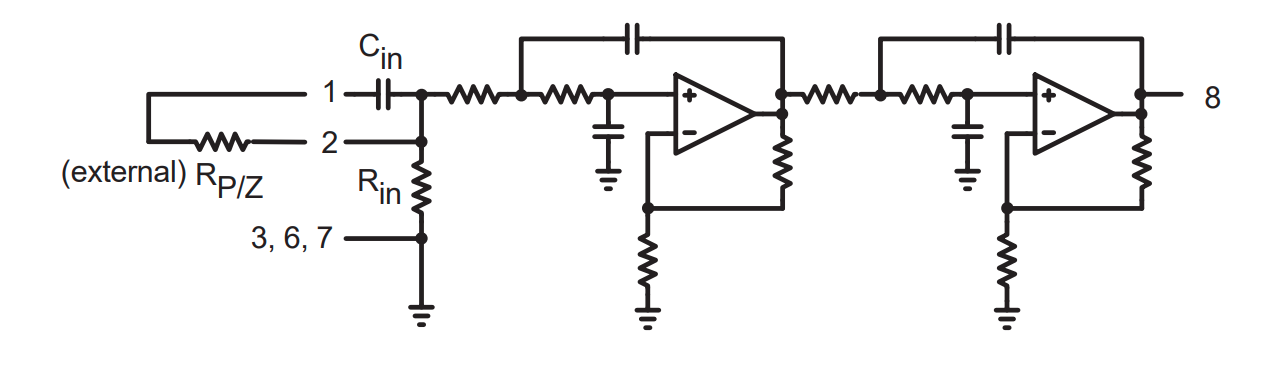
\includegraphics[scale=0.35, angle = 0]{./pictures/CRshaper.png}
 \caption{Internal scheme of CR-200 Gaussian shaping amplifier \cite{cr200}.}
 \label{internal2}
 
\end{figure}

However, shapers are usually very sensitive on the shape of the input pulse. They expect step-like input pulse. The deviation from the expected shapes may result into undefined shapes on output of the shaper. In modules the shapers are usually integrated along with amplifiers.

\subsection{Multichannel analysis (MCA)}
To obtain the full energy spectra information, it is necessary to measure and digitize pulse height of incoming pulses to perform energy discrimination and increment the corresponding channels. The multichannel analyser (MCA) can be employed for these purposes. The EASY-MCA-2K from ORTEC \cite{MCAOrtec}, which we use in experiments, is capable of processing Gaussian shaped pulses with shaping times from 0.25 $\mu$s to 30 $\mu$s and amplitudes ranging from 0 to +10 V.



% %%%%%%%%%%%%%%%%%%%%%%%% End of file %%%%%%%%%%%%%%%%%%%%%%%%

\chapter{Gamma spectrum software analysis}
As was mentioned before, the measured gamma spectrum contains many unwanted artifacts like noise, Compton continuum and edges, additional peaks created by various interactions. To properly obtain the count rates on defined energies the only way is to perform a numerical analysis of measured data.


\section{Peak searching procedure}
Many commercial programs use peak searching procedures based on algorytm originally developed by M.A. Mariscotti \cite{MARISCOTTI1967309}. This method is based on the numerical second difference assuming that the background can be approximated only by linear functions and thus it vanishes in case of the second derivative. The second fact is that the searched peaks are Gaussians with their specific second derivatives and thus their positions can be found in local minimums (Gaussians have negative second derivatives since their are concave functions). To reduce noise, the second difference is averaged by defined number of steps.
\par
To determine if the found minimum should be considered as peak position, standard deviation and other additional rules can be employed. However, algorithm needs input parameters, which are based on raw estimation of FWMH of searched peaks.
\par
For the analysis of measured gamma spectra, this algorithm was implemented in C++ and used to find full energy peaks and other additional peaks as well. The following figures show the example of measured spectra and its second difference plotted along with its standard deviation. The possible candidates onto peak positions can be observed.
\par
\begin{figure}[H]
 \centering
 
\includegraphics[scale=0.105, angle = 0]{./pictures/NoPicture.jpg}
 \caption{Example of measured gamma spectra.}
 \label{Example}
 
\end{figure}

\begin{figure}[H]
 \centering
 
\includegraphics[scale=0.105, angle = 0]{./pictures/NoPicture.jpg}
 \caption{Second difference of example spectra along with its standard deviation showing possible candidates.}
 \label{secondDerivative}
 
\end{figure}

\section{Intensities calculation}


\chapter{Gamma detection testing}

The purpose of this experiment is to determine the necessary conditions under which the gamma spectroscopy with selected photodiodes can be performed and find out whether the photodiodes are even capable of detecting gamma rays since the purpose of some them is not defined as a detector of gamma rays. The determination of detection efficiency is precisely done in following chapters for selected photodiodes. 
\par
For the very first test of photodiodes we assembled a spectrometric setup from ORTEC modules including preamplifier ORTEC142A, shaping amplifier 575A and high voltage source inside the ORTEC minibin. The pulses were captured by ORTEC MCA connected to PC running the MAESTRO Multichannel Analyzer Emulation Software \cite{maestro}. 


\begin{figure}[H]
 \centering
 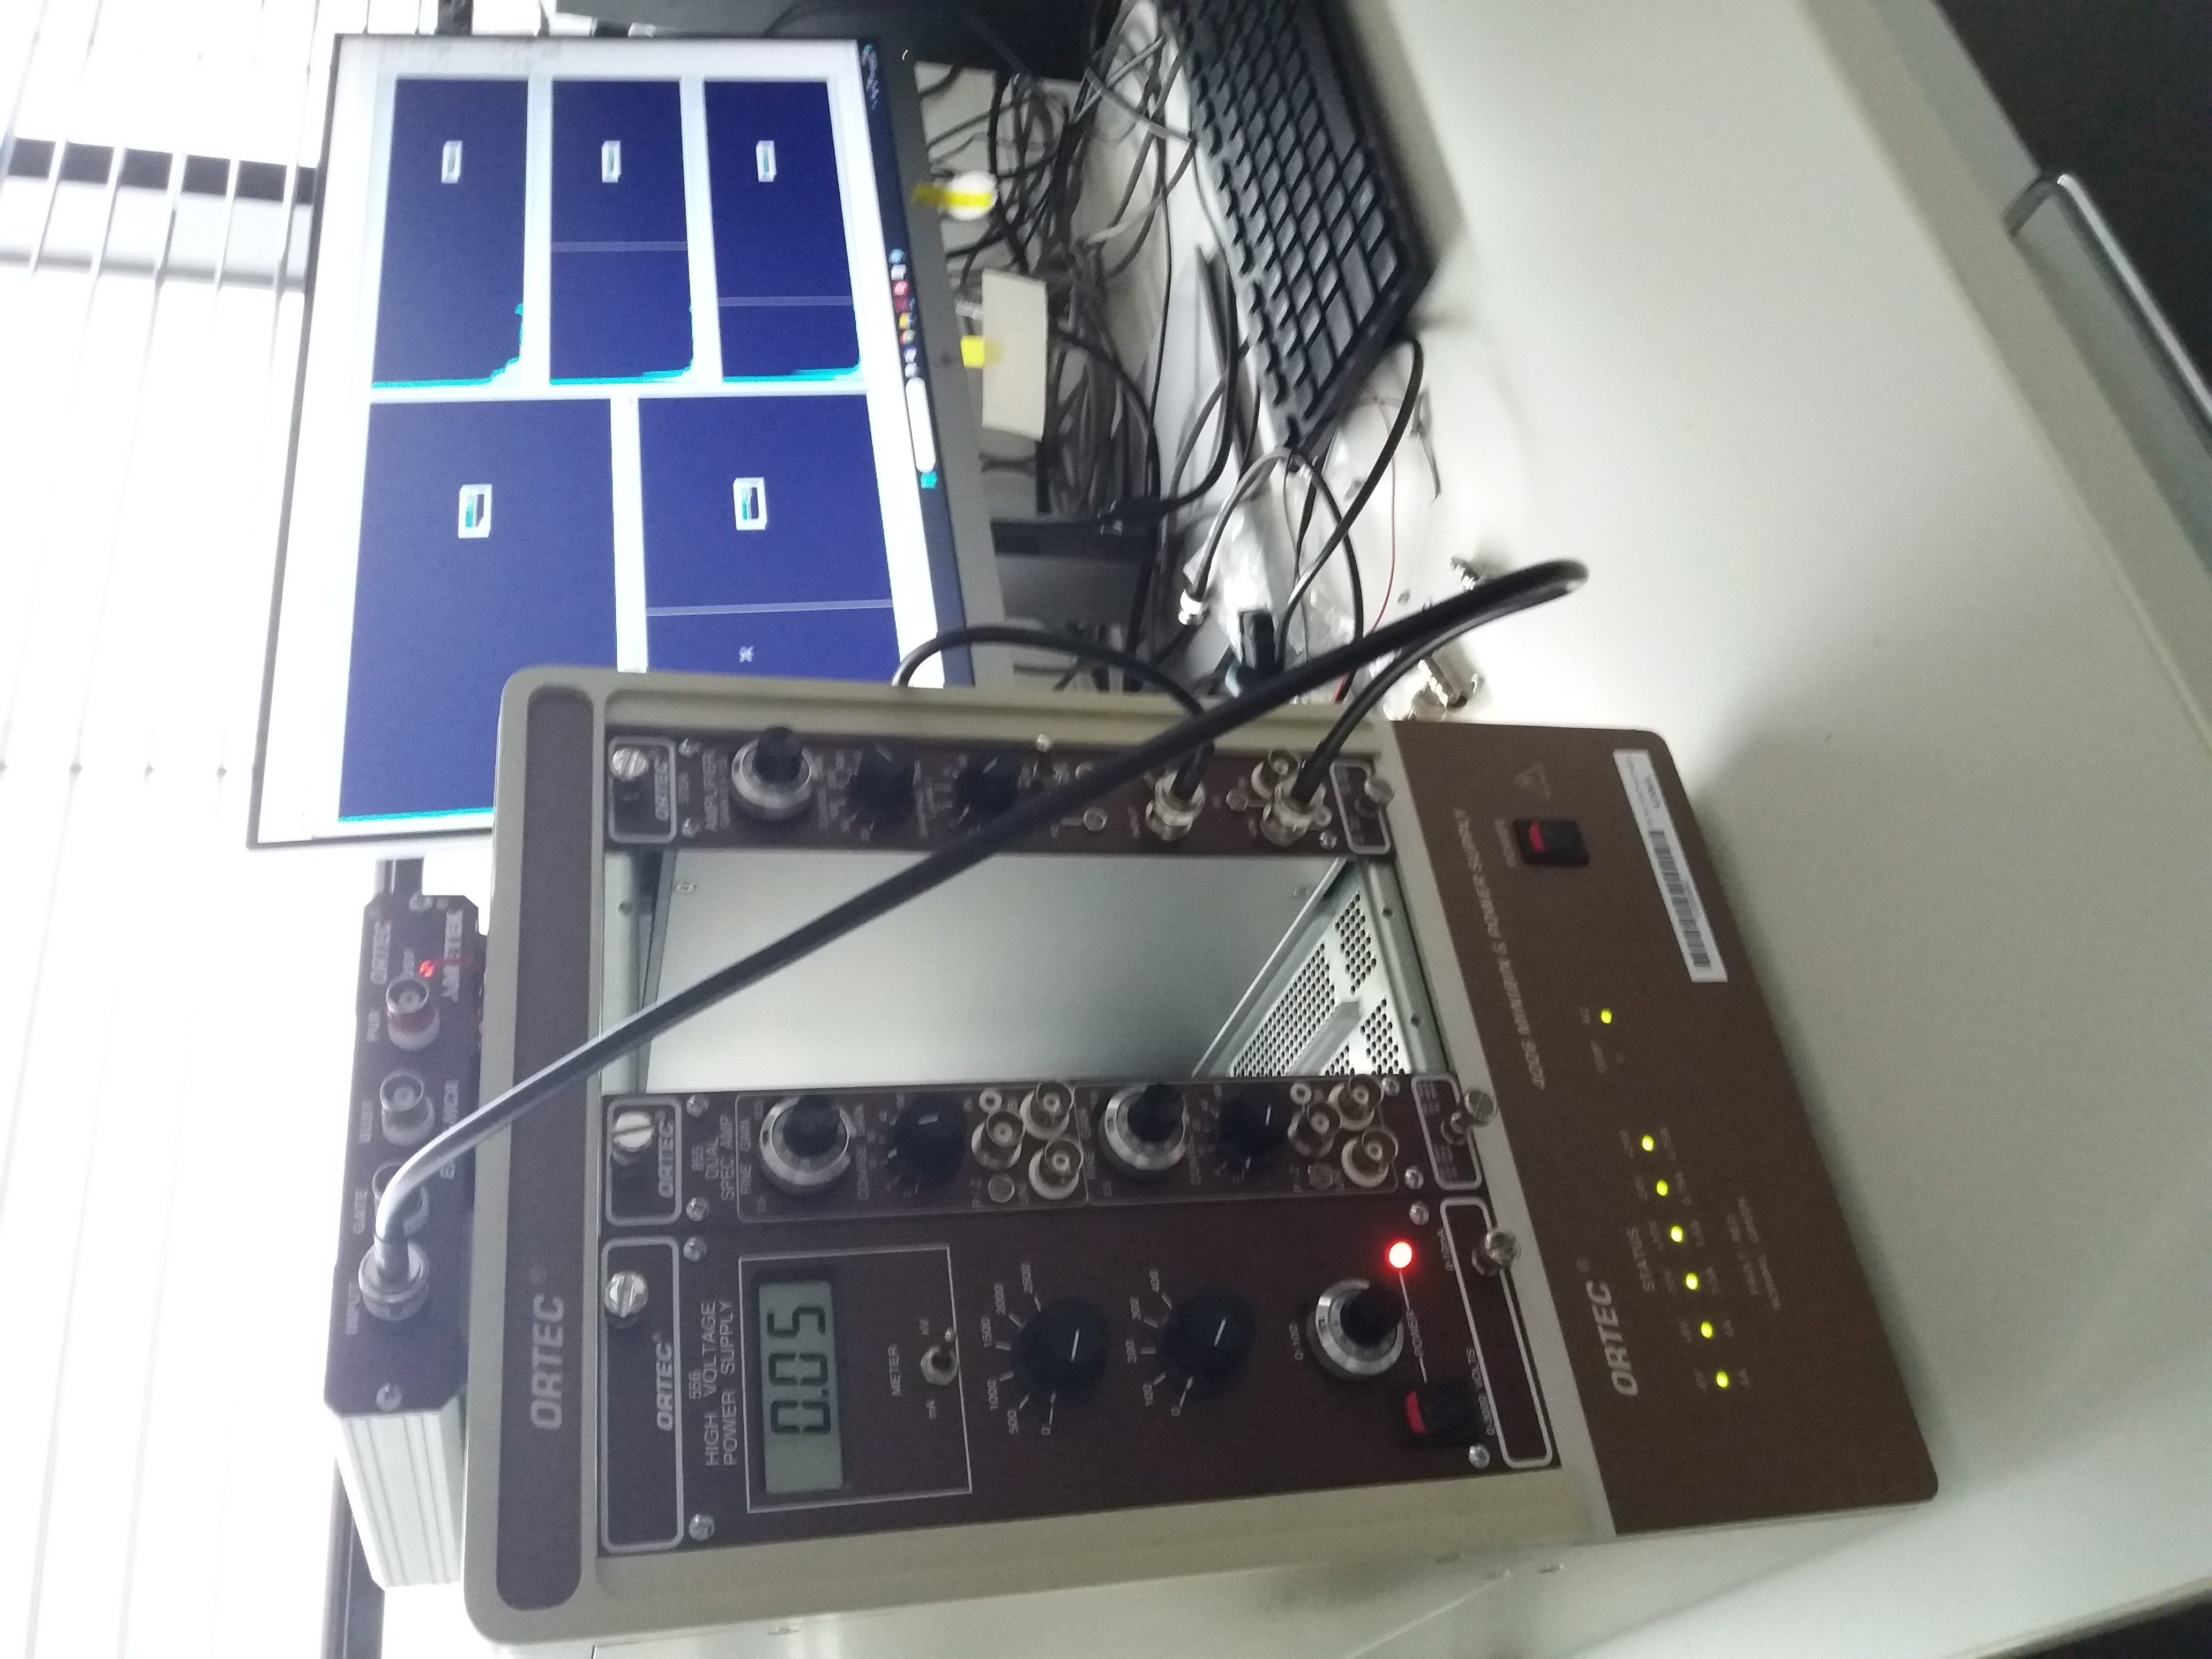
\includegraphics[scale=0.09, angle = 270]{./pictures/ORTECbin.jpg}
 \caption{ORTEC minibin with MCA connected to PC.}
 \label{minibin}
 
\end{figure}
\par
As radiation source we use $^{57}$Co 50 mCi Mössbauer source from 2016 and thus it was necessary to cover the part with radiation source with lead shielding blocks.



\begin{figure}[H]
 \centering
 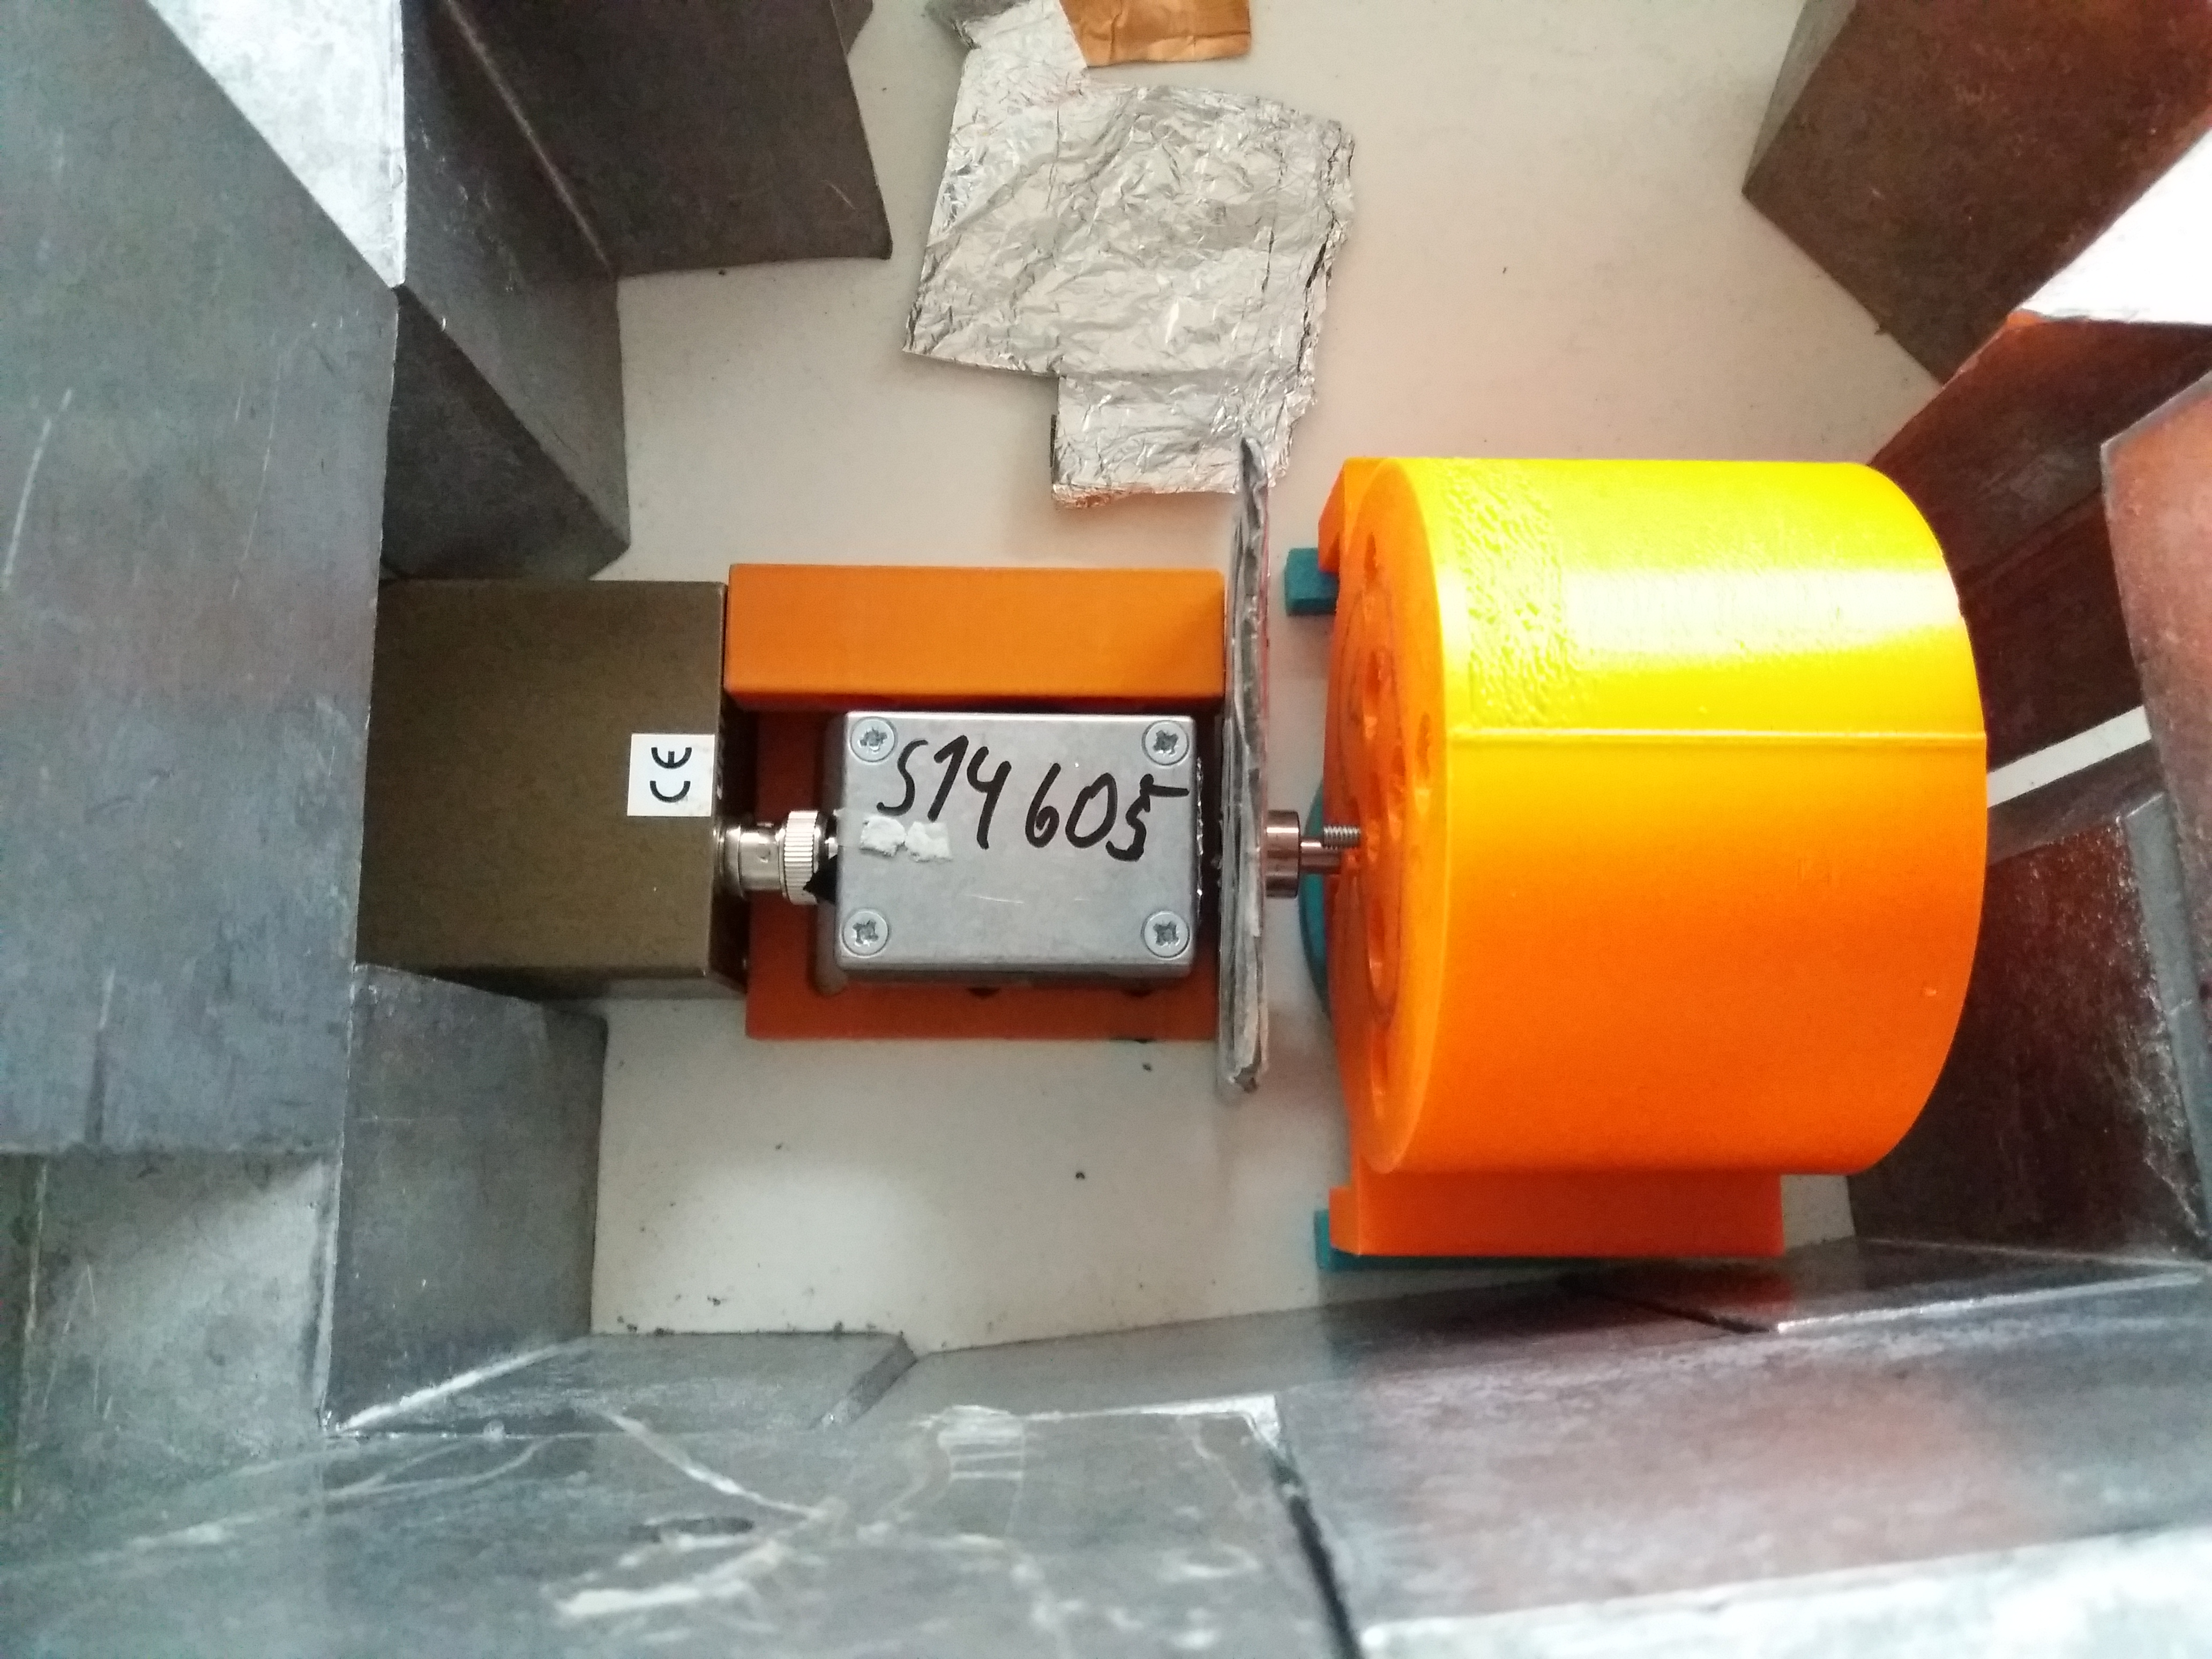
\includegraphics[scale=0.09, angle = 0]{./pictures/ORTECsetup.jpg}
 \caption{PIN diode inside the shielding crate connected to the preamplifier to measure the $^{57}$Co source with filter.}
 \label{setup}
 
\end{figure}


\section{Noise and its reduction}
When performing gamma spectroscopy measurements, the energy spectra are affected by noise. In order to reduce noise as much as possible, two approaches were tested - shielding the detector by various ways and cooling to temperatures near 0  $^\circ$C.
\subsection{Electromagnetic noise reduction}
Photodiodes have to be sufficiently electromagnetically shielded and their distance to the preamplifier input should be as short as possible. Using the diodes with poor shielding leads into high levels of electromagnetic noise, which make mayor part of energetic spectra unobservable.
\par
On the behalf of many tests it was proven that the best way to shield the photodiode is to put it into the aluminium crate (see \ref{crate}). This crate has to be small as possible and has to be connected to the grounding potential. However, the front side of the crate has to be open to allow the sufficient transmission of gamma photons to the detector. A drilled hole covered by a thin aluminium foil has sufficient gamma transmission parameters as well as electromagnetic shielding parameters.

\begin{figure}[H]
 \centering
 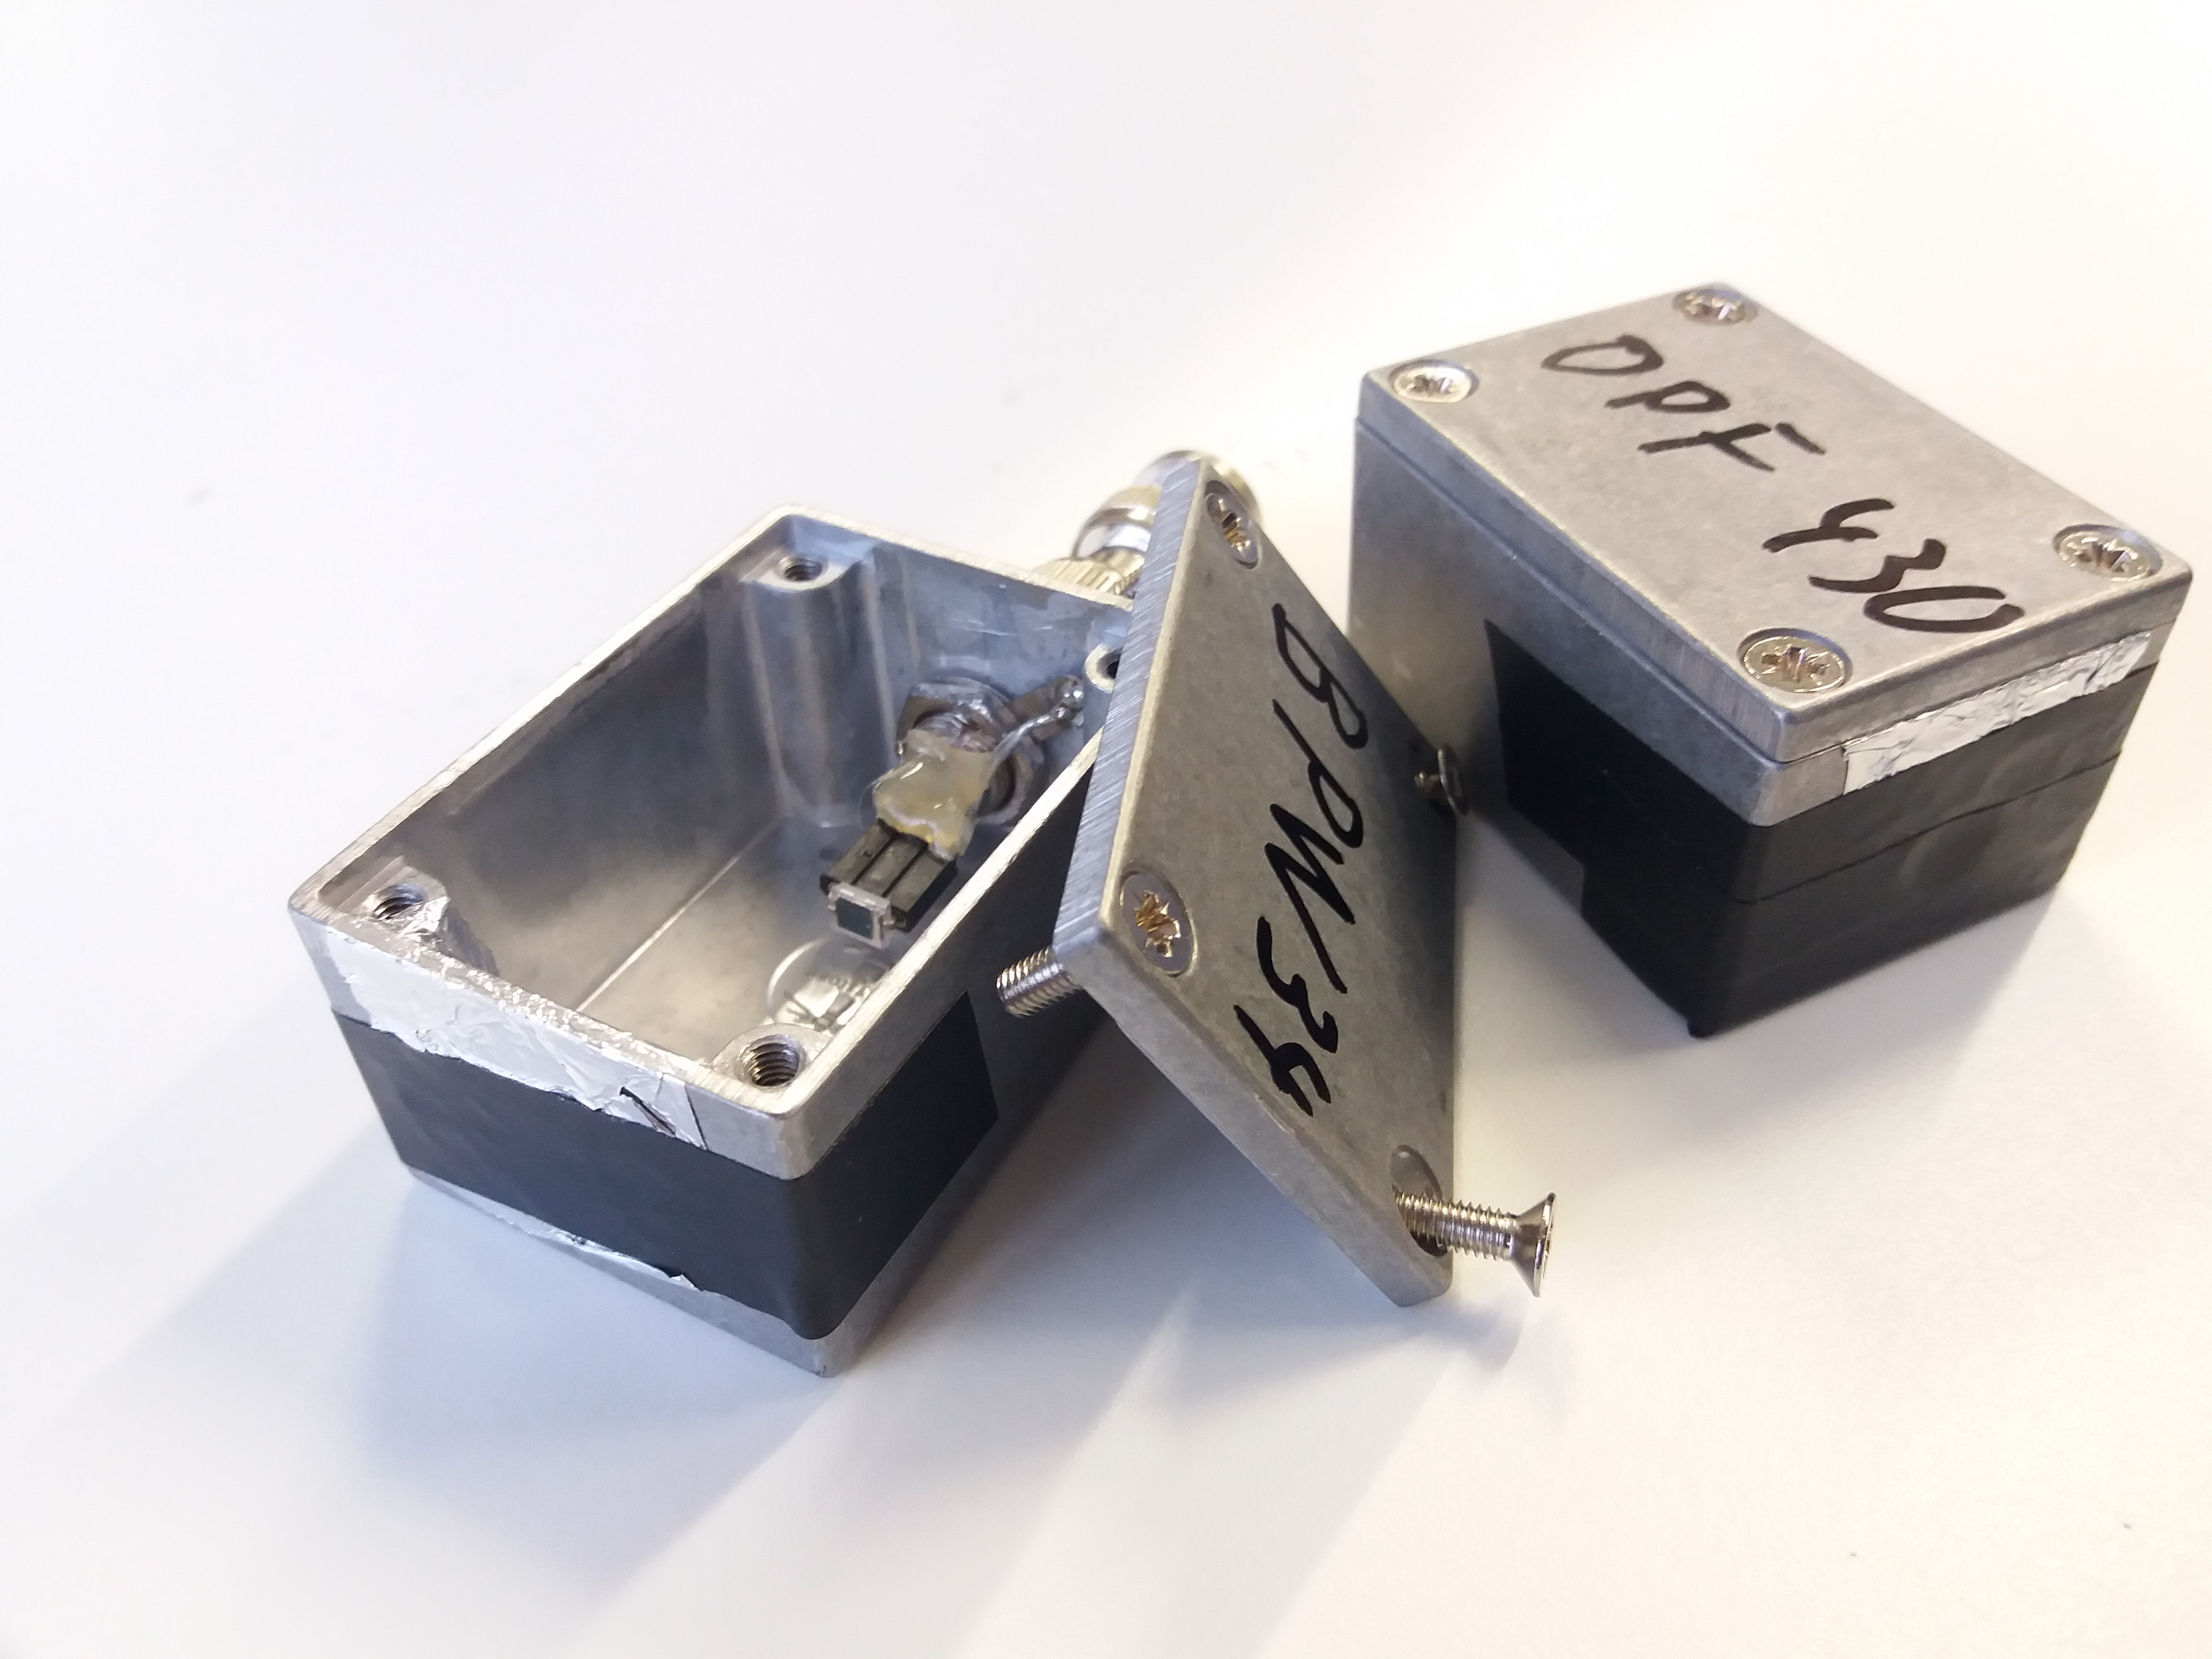
\includegraphics[scale=0.09, angle = 0]{./pictures/ShieldCrate.jpg}
 \caption{Photodiode inside aluminium shielding crates.}
 \label{crate}
 
\end{figure}


%\begin{figure}[H]
% \centering
% 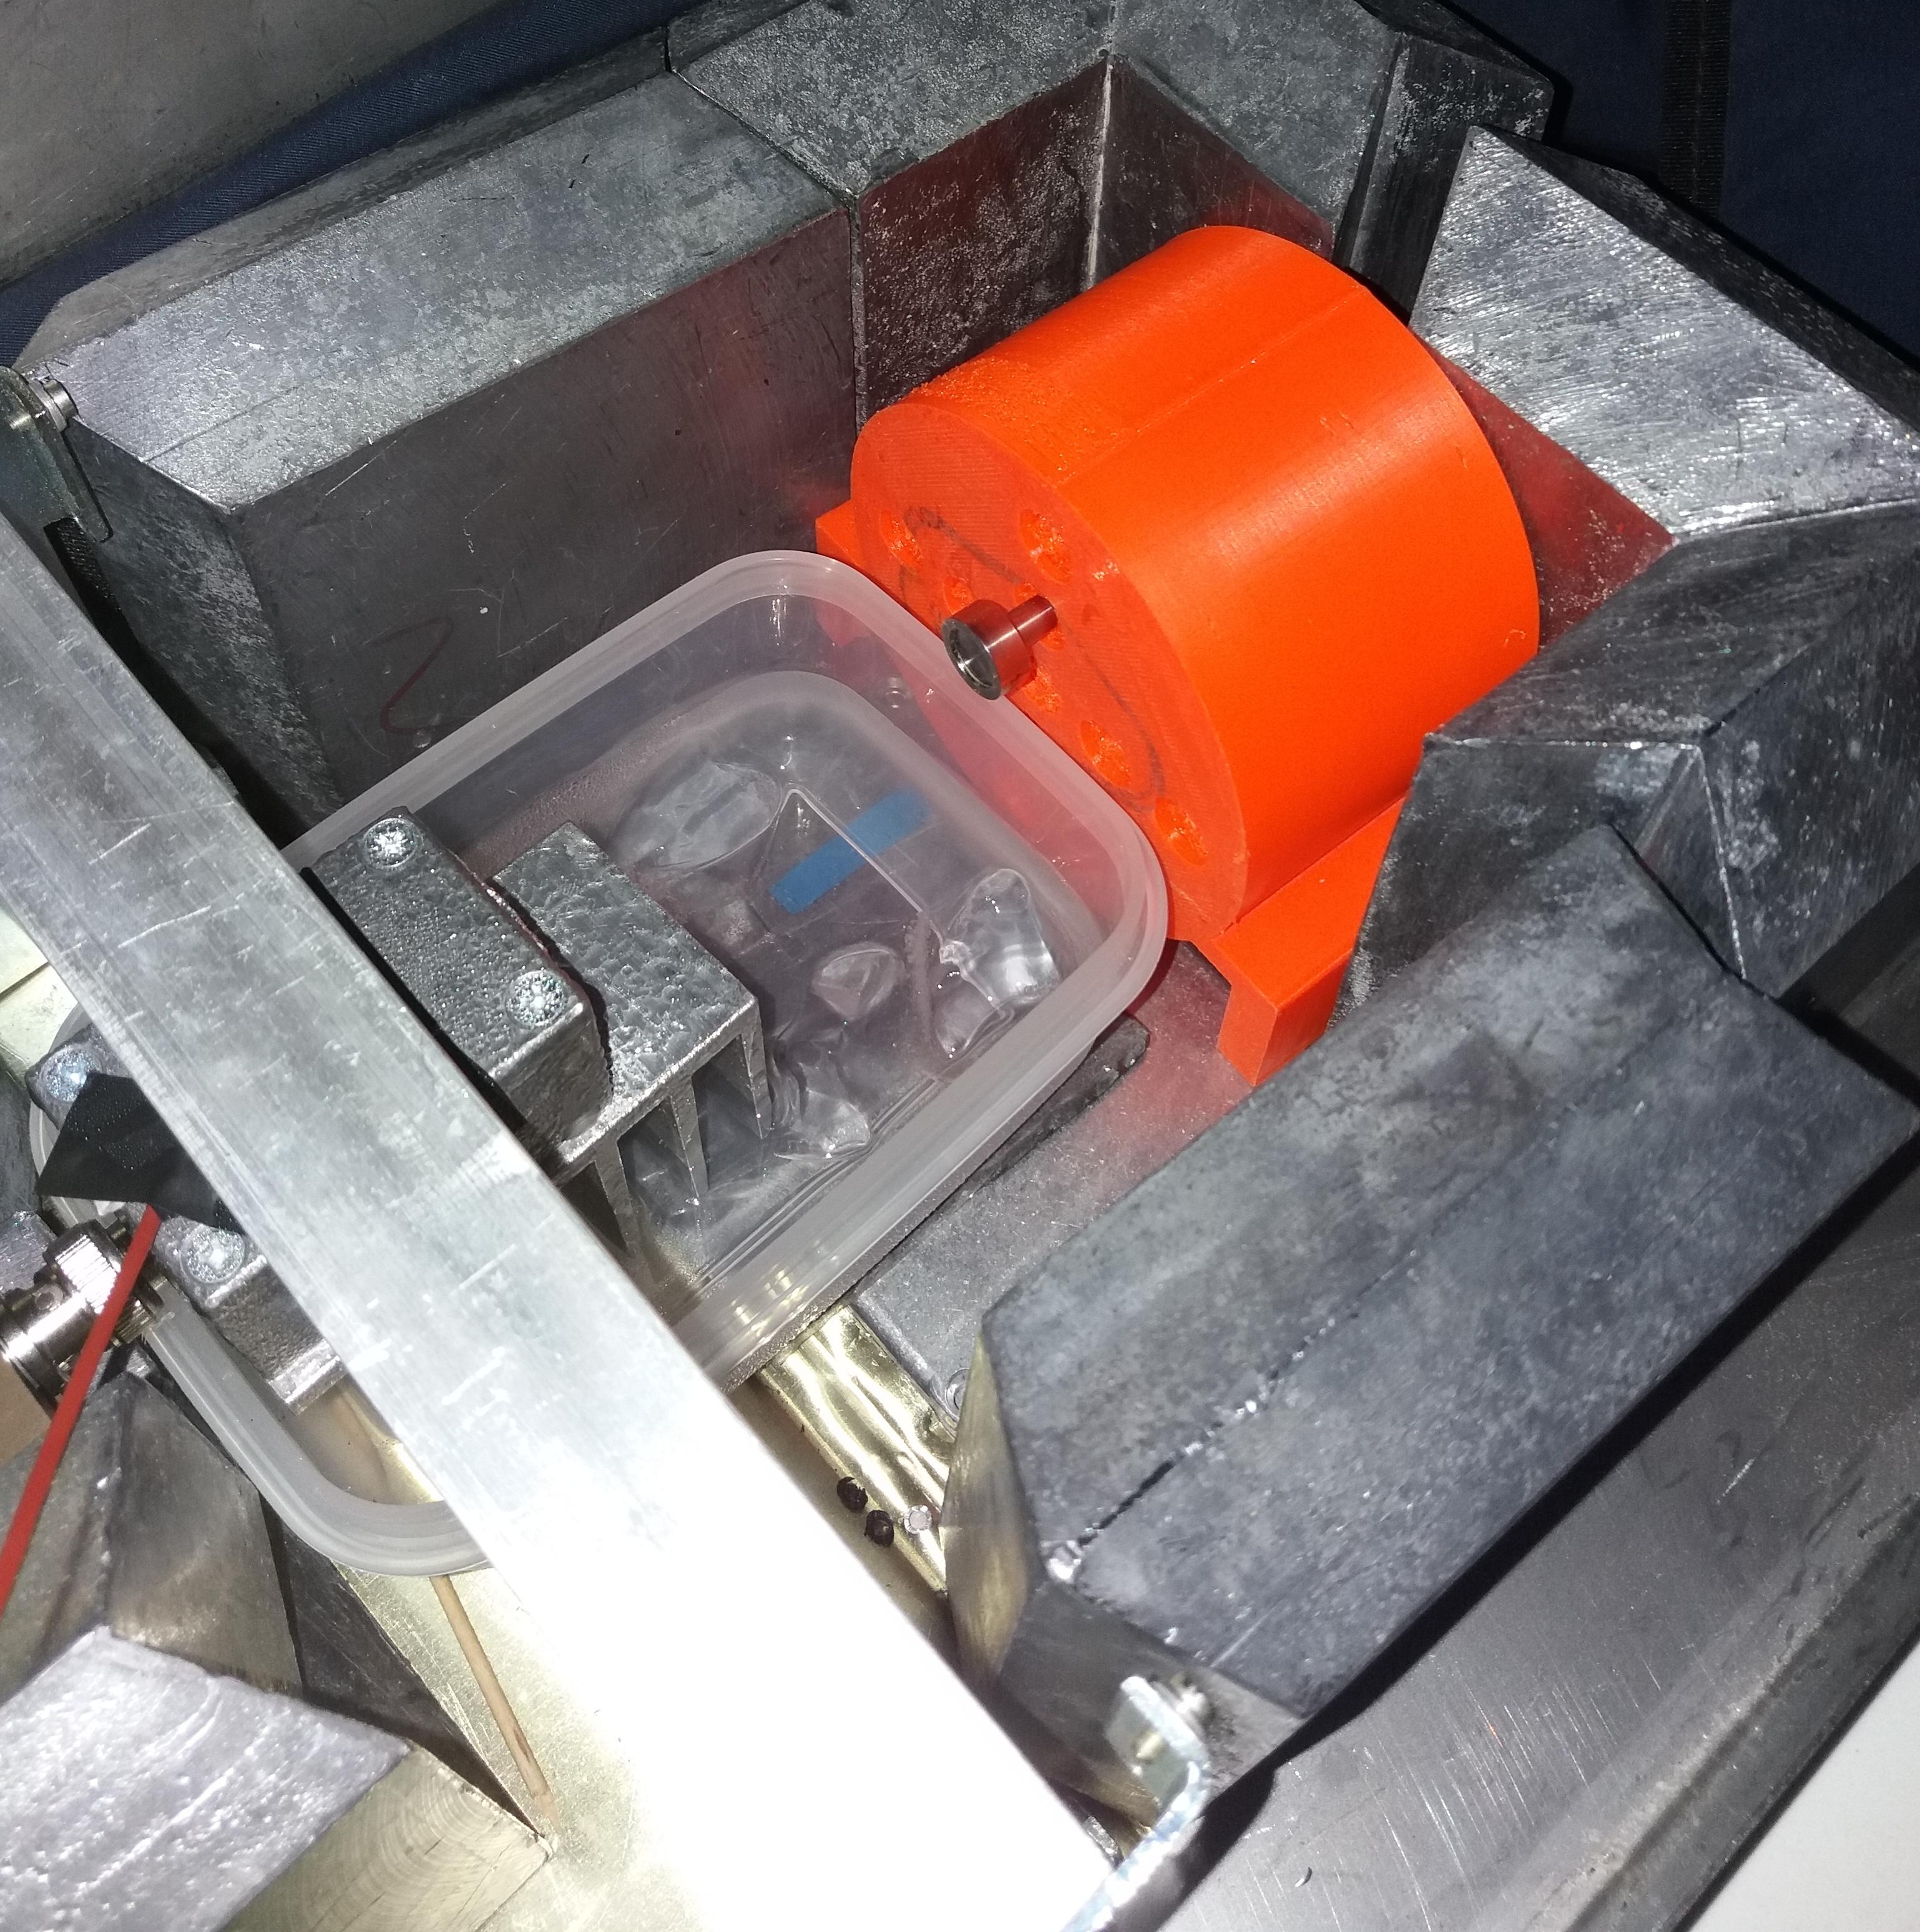
\includegraphics[scale=0.09, angle = 0]{./pictures/chlazeniLedem.jpg}
% \caption{Example of $^{57}$Co spectra from poorly shielded detector setup and from sufficiently shielded detector.}
% \label{notShielded}
% 
%\end{figure}





\subsection{Thermal noise reduction}
To reduce the thermal noise, the S14605 photodiode was cooled by ice. It was placed in shielding box, which had attached heat sink to the bottom. This heat sink was submerged into the small tub filled with a melting ice (picture \ref{cooler}). The thermal conduction was improved by sticking the photodiode to the of the floor of the shielding box by conduction paste. The photodiode was cooled this way to temperatures around 7-8 $^\circ$C.


\begin{figure}[H]
 \centering
 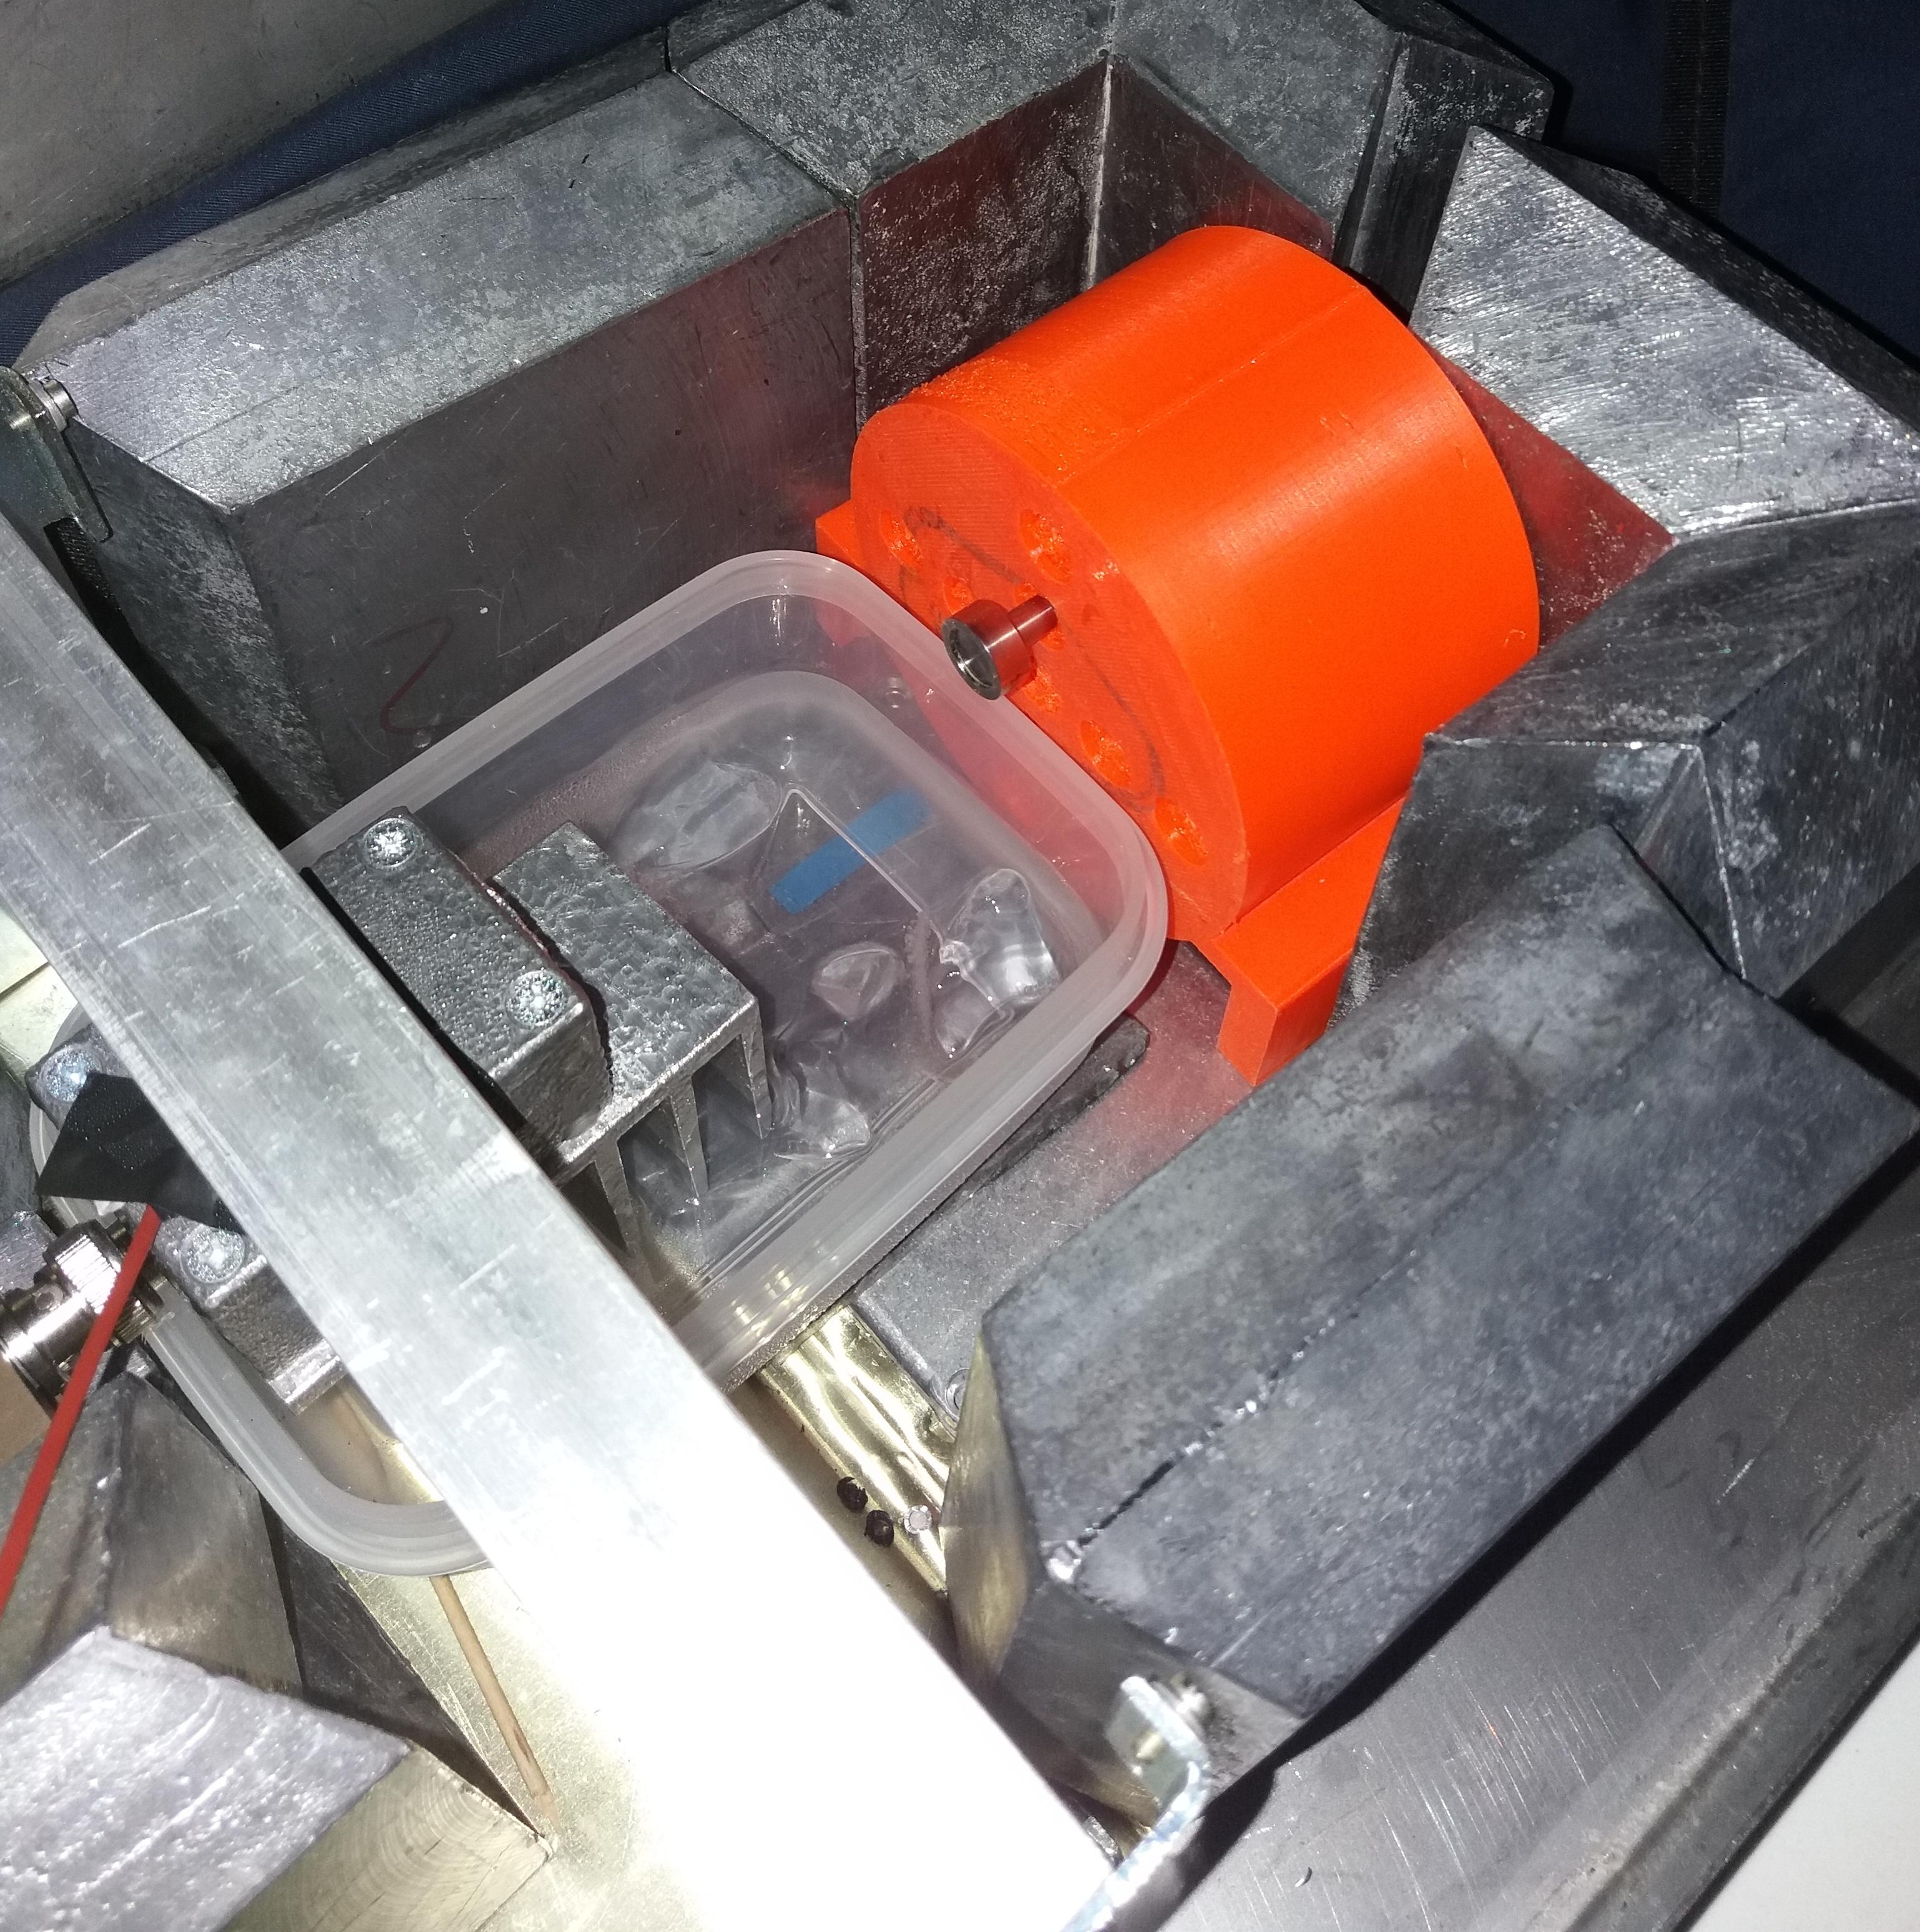
\includegraphics[scale=0.09, angle = 0]{./pictures/chlazeniLedem.jpg}
 \caption{Detector cooled by ice.}
 \label{cooler}
 
\end{figure}



\begin{figure}[H]
 \centering
 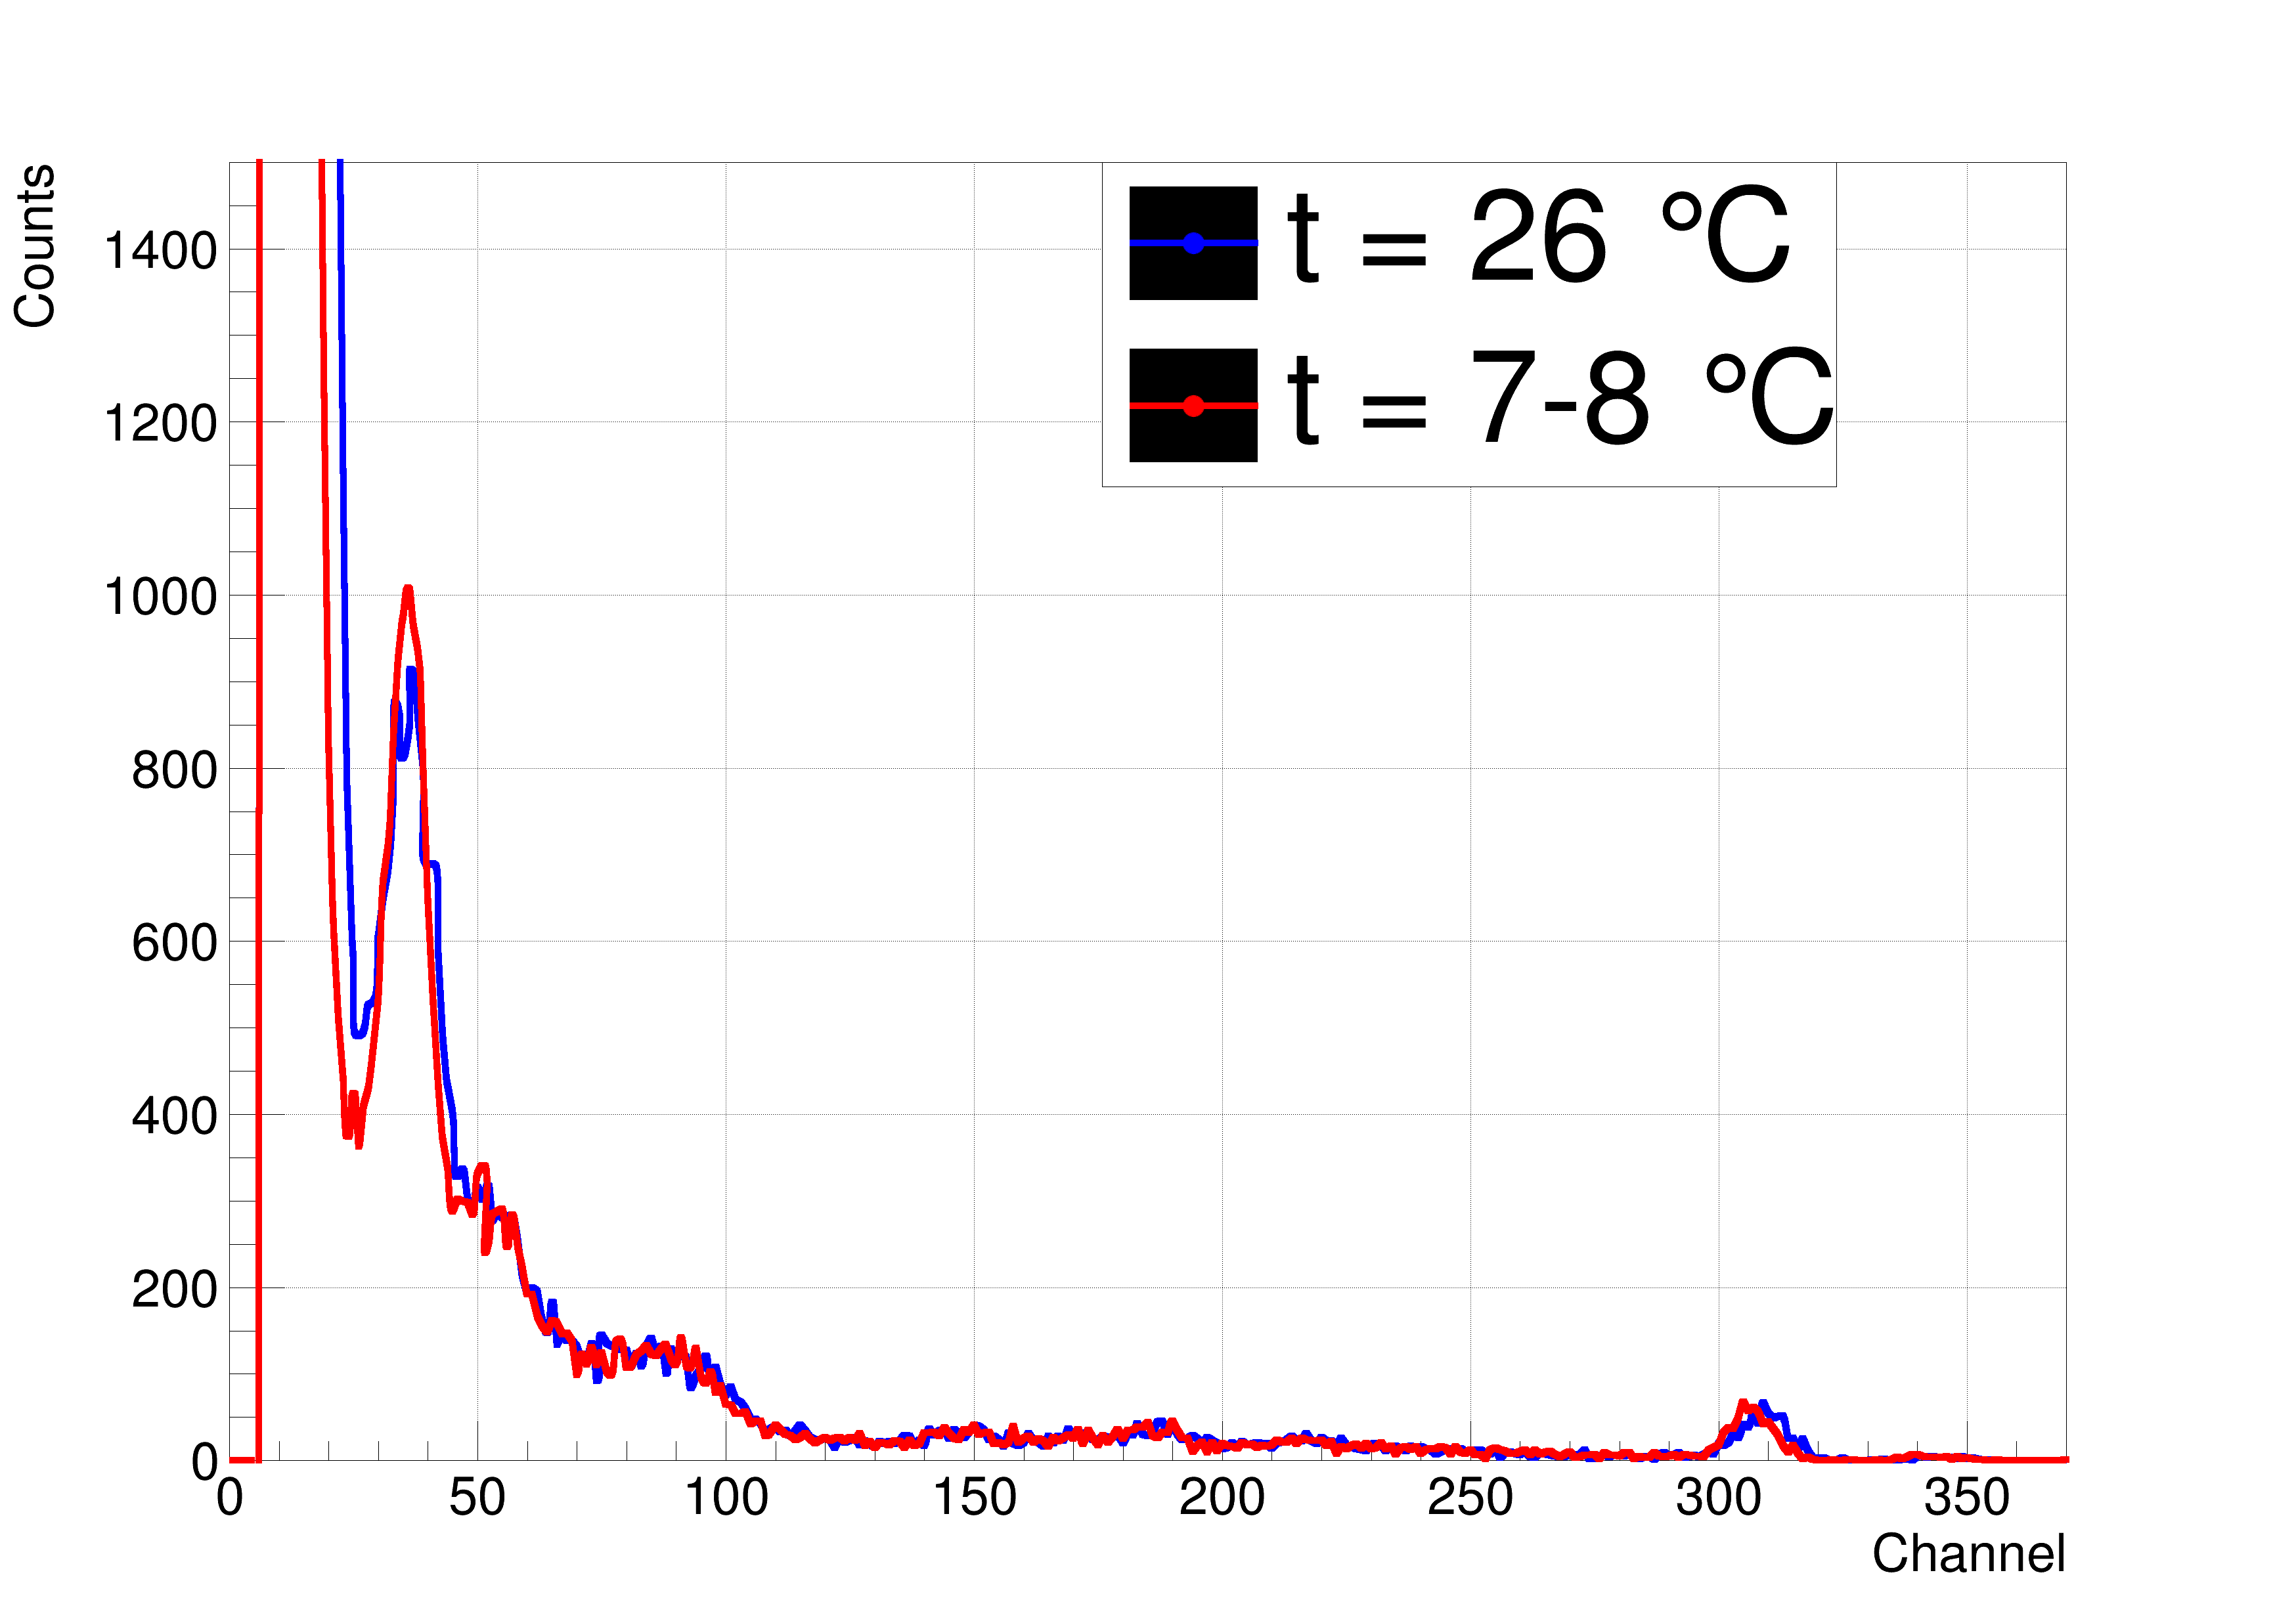
\includegraphics[scale=0.13, angle = 0]{./pictures/TempDiff.png}
 \caption{Measured $^{57}$Co spectra at two different temperatures.}
 \label{coolspectr}
 
\end{figure}








\par
The results show that the cooling improves SNR, but its effect is small when compared to the effect of proper shielding. The cooling is not used in following tests on ORTEC setup.
%It was also tried to use the peltier cooler instead, however, the cooling efficiency was low when compared to the ice.

\section{Detection test of the $^{57}$Co spectra}
The spectra for every photodiode taken for 30 min of real time (MCA allows dead time compensation) with the source's distance 1 cm from the front shielding crate. There is a simple test with a set of filters, which can help us to find out the corresponding energies to the measured peaks:

\begin{itemize}
\item Pb filter: everything should be attenuated.
\item Cu filter: transmitted - 122.1 keV, 136.5 keV not transmitted - 14.4 keV, 6.4 keV.
\item Al filter: transmitted - 122.1 keV, 136.5 keV, 14.4 keV not transmitted - 6.4 keV.
\end{itemize}

The analysed spectre is analysed by peak finder program to find the characteristic energy components. By filter test it can be determined which peak corresponds to 14.4 keV (Cu - attenuated, Al - not attenuated). The channel position of 14.4 keV is then used to recalculate the other peak's channel positions to energies.
\par
The Compton edge caused by interaction of 122.1 keV photons inside the detector can be expected. The equation \ref{compton} estimates the position to be around 39.5 keV. 

\subsection{S14605 test}
From the S14605 capacity graph \ref{datS14605} can be deduced optimal voltage - we decided to set it to 50 V. It was observed that any further increase of voltage do not improves the SNR. The measured spectra with no filter and with attached 3 filters plus background are on the fig. \ref{S14605 spectra}.


\begin{figure}[H]
 \centering
 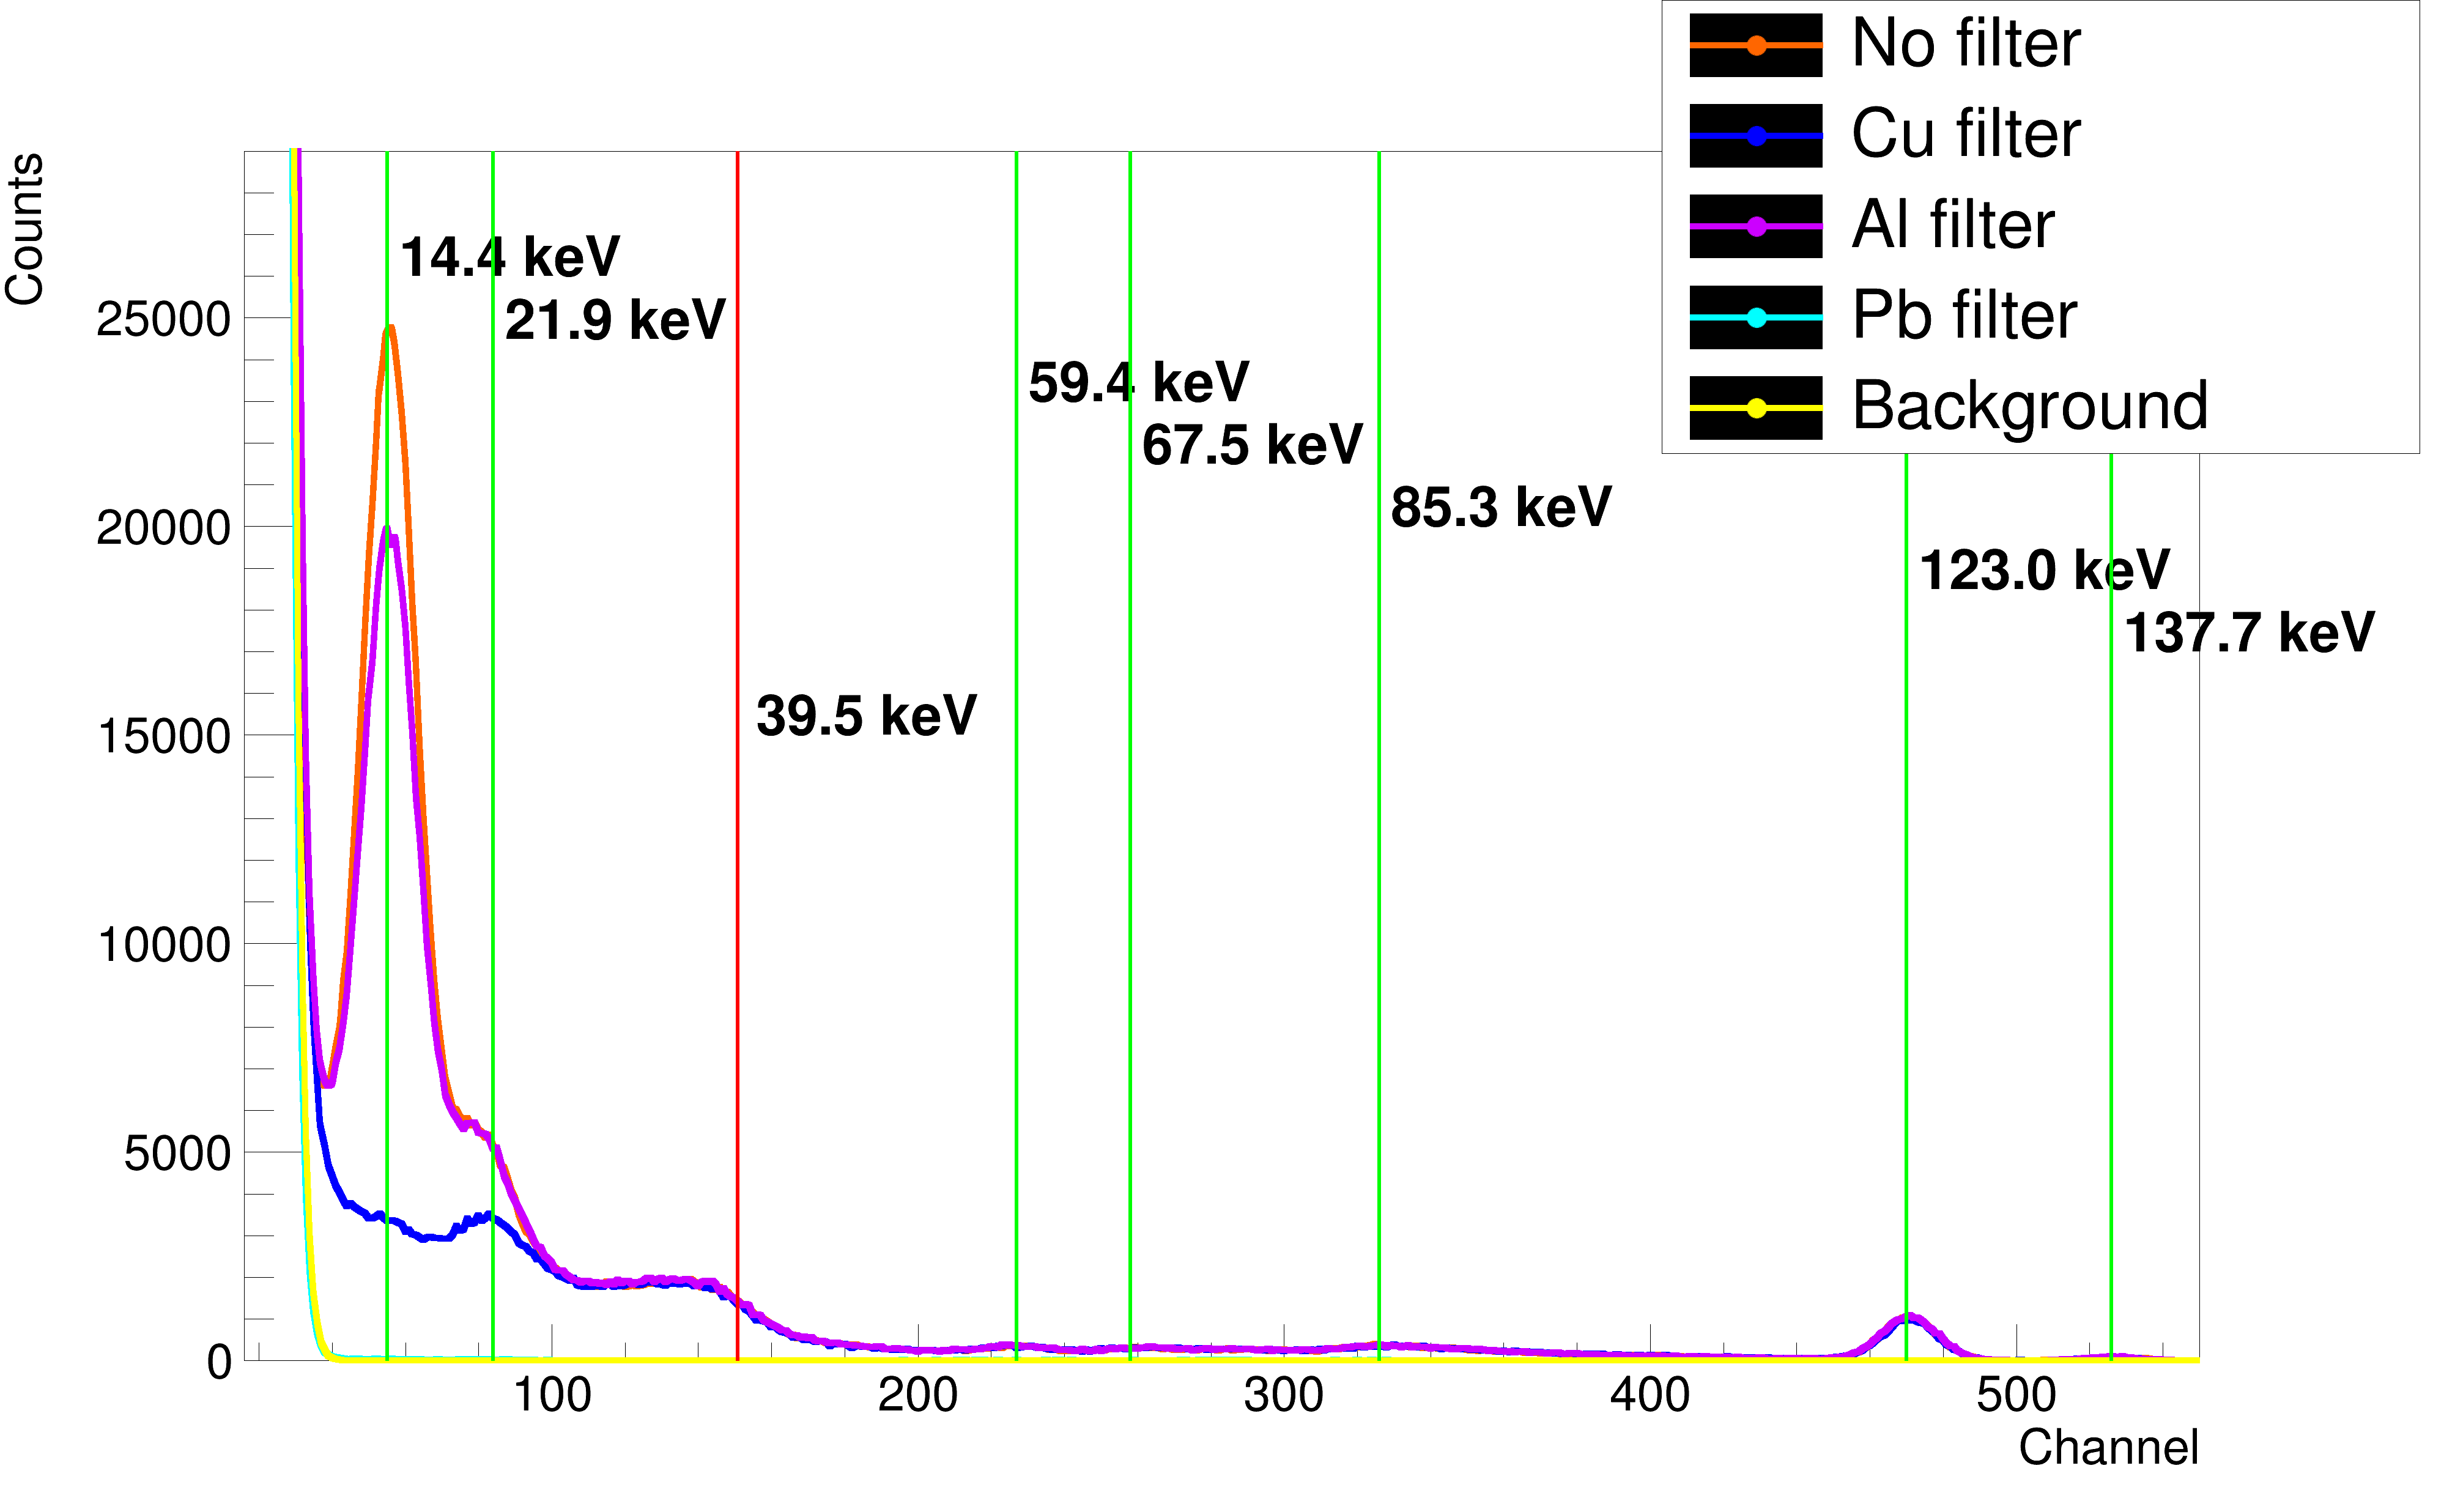
\includegraphics[scale=0.125, angle = 0]{./pictures/S14GammaTest.png}
 \caption{S14605 spectra with founded energy peaks (green lines) and estimated Compton edge (red line).}
 \label{S14605 spectra}
 
\end{figure}


\par

Due to the first peak's attenuation by mentioned filters it can be considered as 14.4 keV full energy peak. The 21.9 keV peak originates from characteristic RTG of rhodium matrice. 59.4 and 67.5 keV 85.3 keV is characteristic RTG of lead shielding. The last two peaks (123.0 keV, 137.7 keV) are from $^{57}$Co. It can be seen that the full energy detection efficiency of higher energies (122 keV) is very small and that the Compton scattering is preferred interaction effect inside detector at these energies, which results into expected Compton edge. The expected peak of 6.4 keV was unfounded possibly due to the insufficient SNR. The modular ORTEC setup do not allows any further upgrades, so the only way to improve SNR is to integrate the spectrometric chain into PCB. 

\subsection{BPW34 test}
The instrumentation was similar as before, but BPW34 had to be operated at lower bias voltage - 20 V.

\begin{figure}[H]
 \centering
 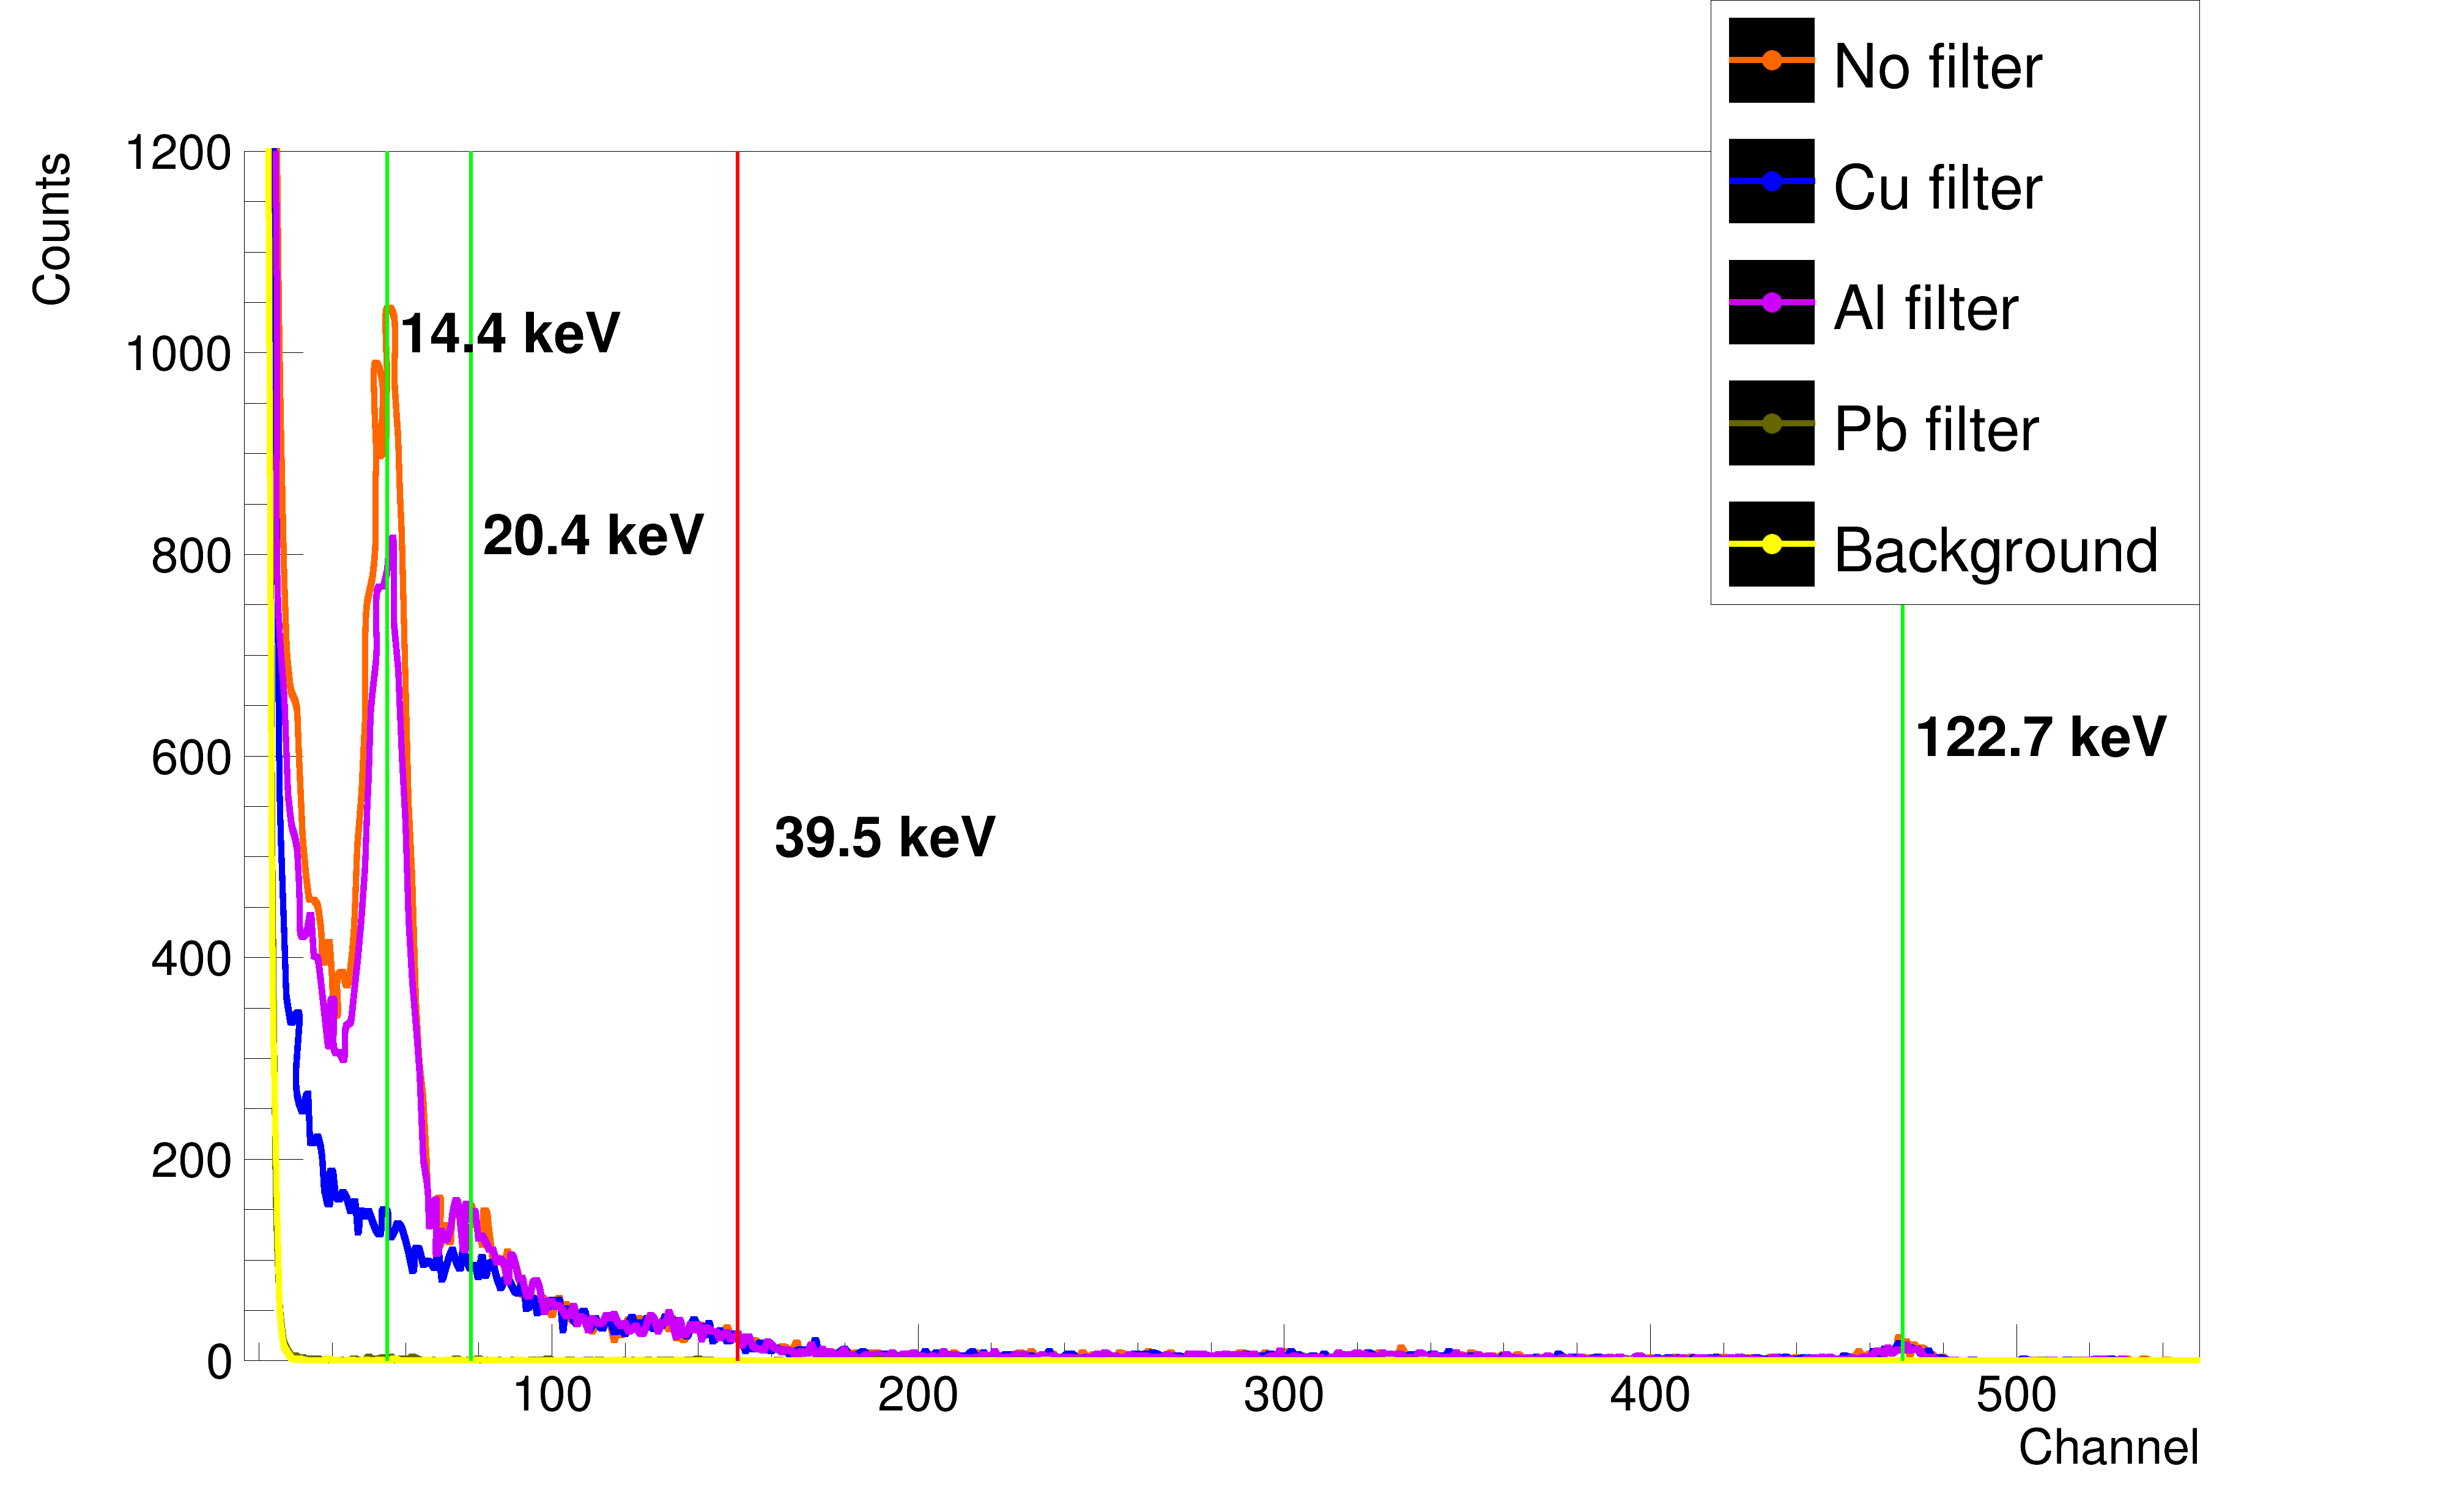
\includegraphics[scale=0.125, angle = 0]{./pictures/BPW34GammaTest.png}
  \caption{BPW34 spectra with founded energy peaks (green lines) and estimated Compton edge (red line).}
 \label{BPW34 spectra}
 
\end{figure}

The measured spectra of BPW34 is very similar to the previous one, however the peak's heights are about 25 times lower.

It is surprising that this cheap photodiode is capable of capturing gamma rays with sufficient energy resolution. The efficiency is lower than S14605 about .
\subsection{OPF430 test}
OPF430 was operated on 20 V. There was a problem with the very low detection efficiency, so the source had to be put into the shielding box right before the photodiode.

\begin{figure}[H]
 \centering
 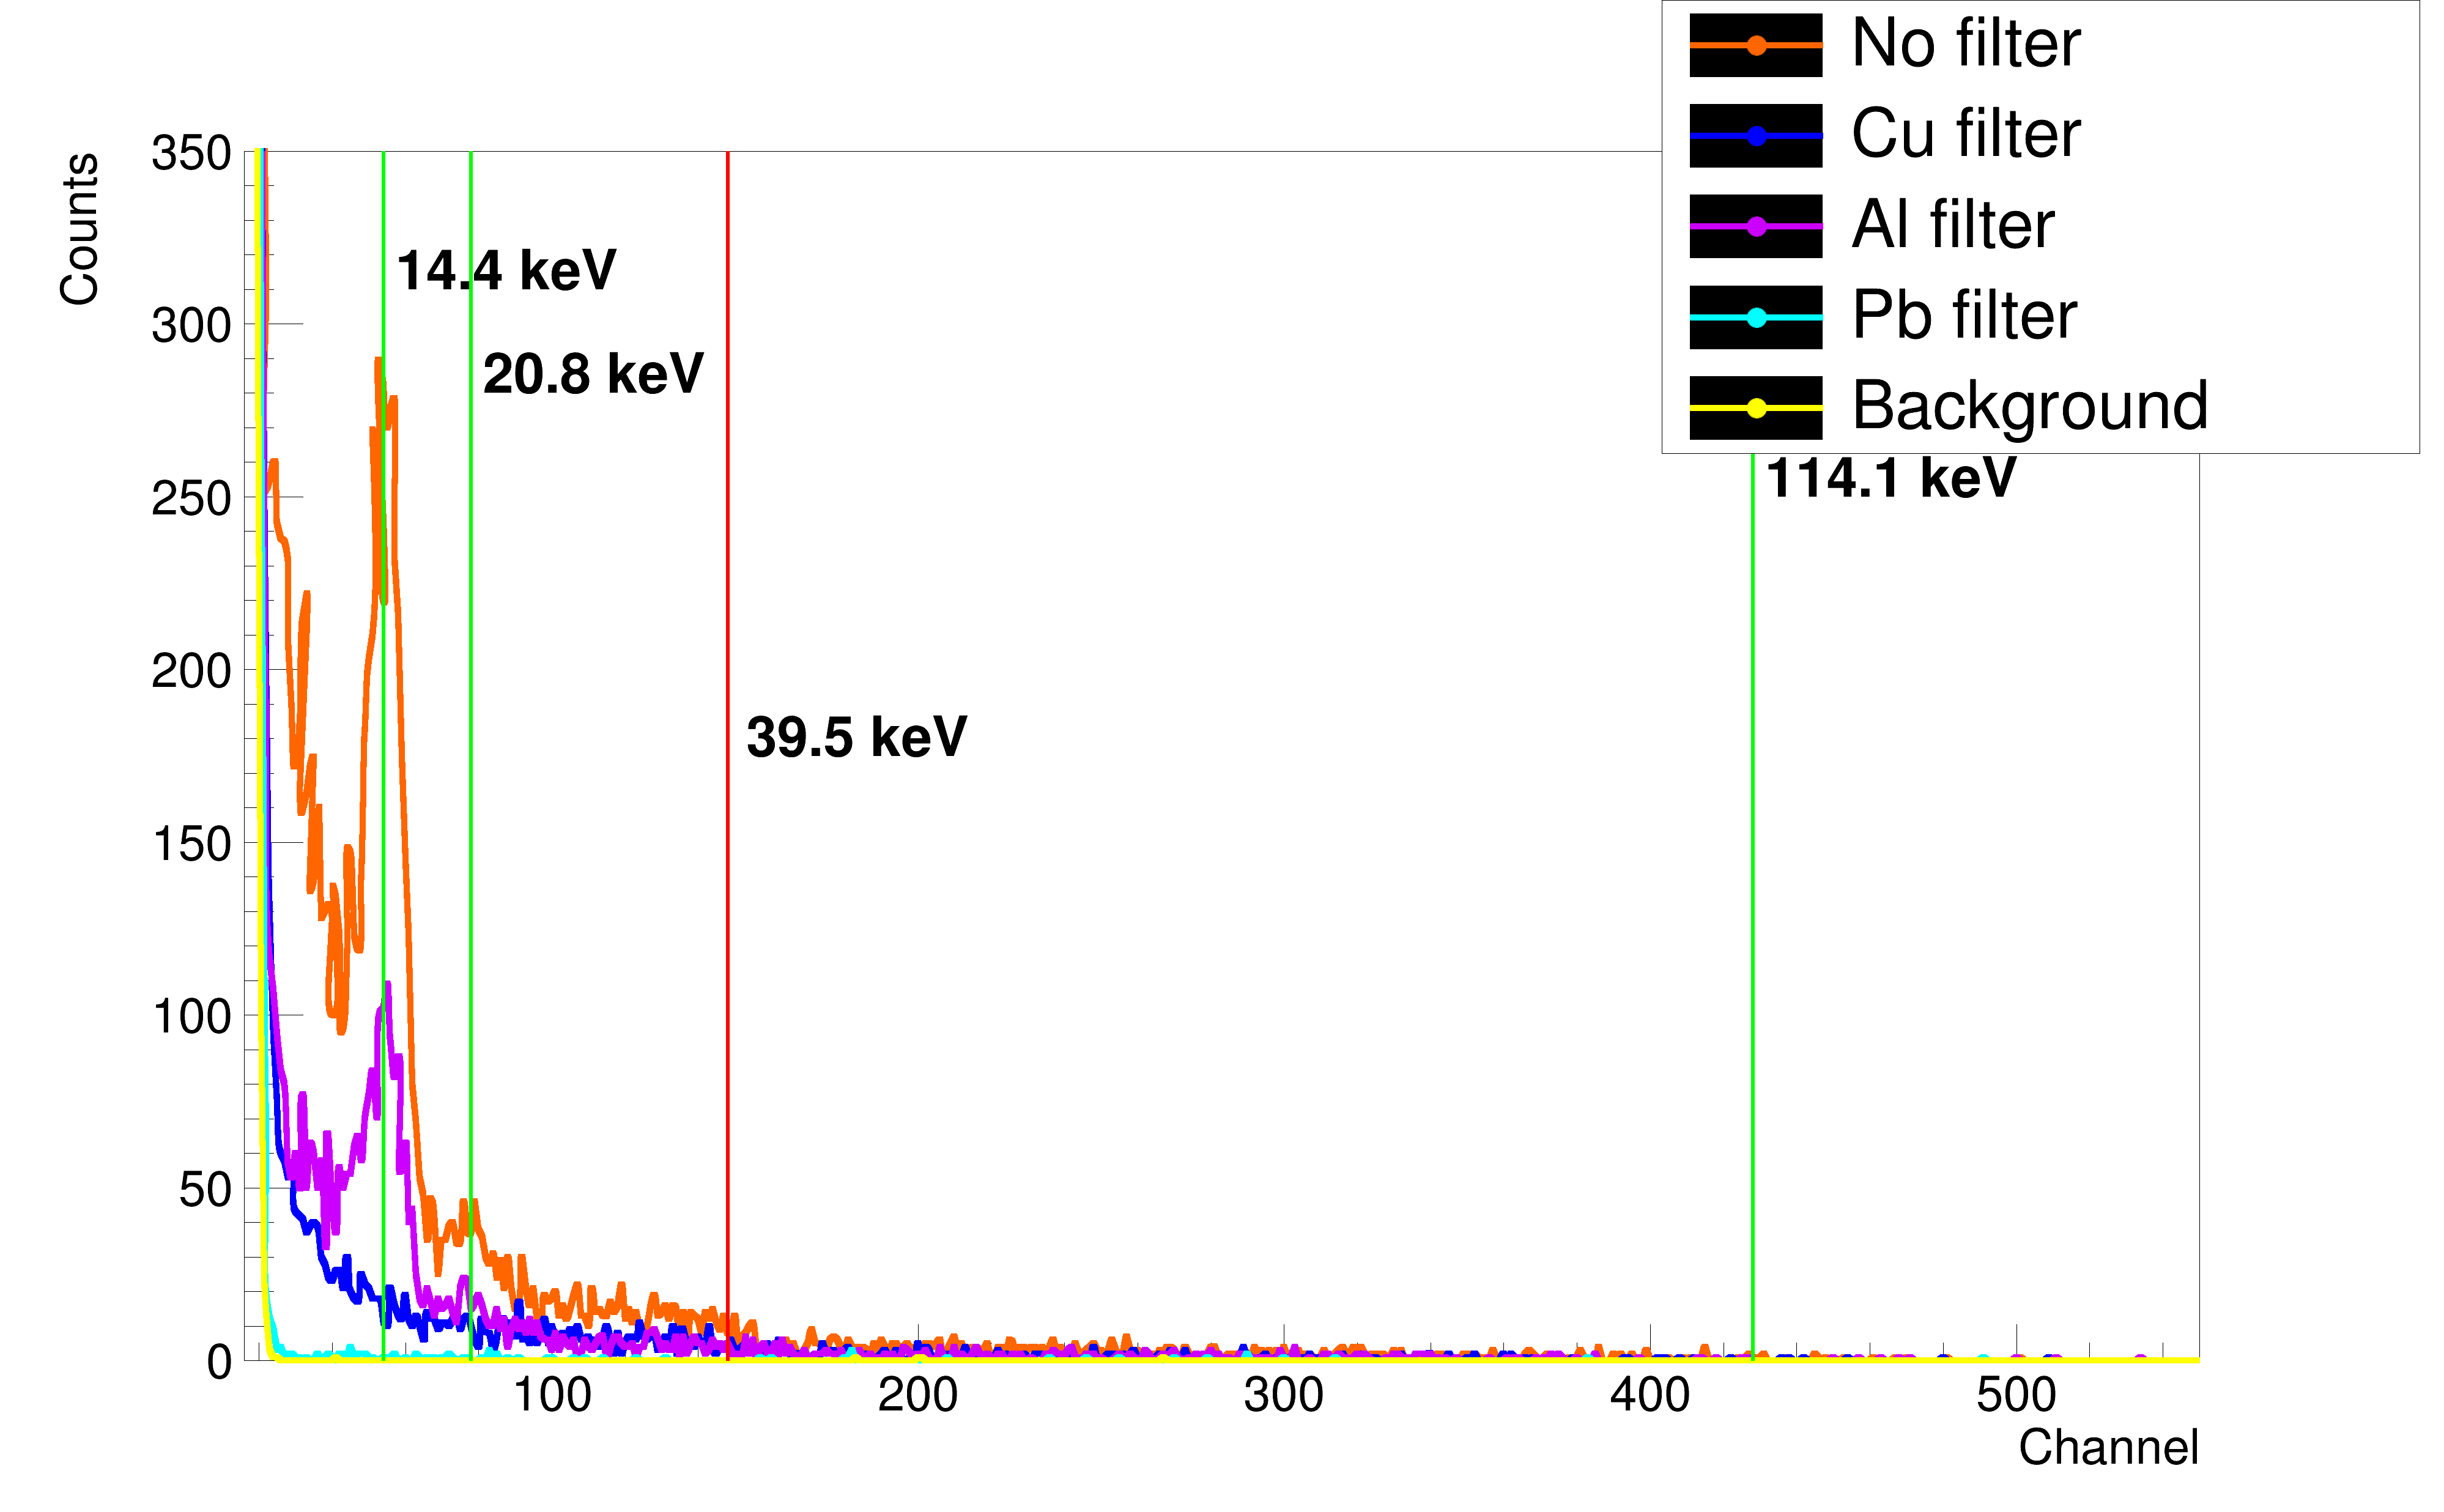
\includegraphics[scale=0.125, angle = 0]{./pictures/OPF430GammaTest.png}
 \caption{OPF430 spectra with founded energy peaks (green lines) and estimated Compton edge (red line).}
 \label{OPF430 spectra}
 
\end{figure}

It can be seen that the count rates are still much lower that they were measured at previous photodiodes. This is probably due to the fact, that the surface of detector is very small.
The conclusion is that OPF430 is capable of capturing the low-energy gamma rays, however, the efficiency is so bad that it makes it unusable for any real gamma spectroscopy application. 


\chapter{Design of integrated amplifier}
The only way to improve the performance of the spectrometric chain is to integrate the amplification part and a shaper into a small PCB - short the signal routes, reduce parasitic capacitances at preamplifier input and improve the shielding. The various prototypes were designed as double-sided PCBs and manufactured by using the milling machine for PCB to remove cooper from cuprextit plates. The PCB consisting mainly of surface mount deposition (SMD) parts was then assembled by manual soldering.

\section{Scheme and layout}
The main parts of spectrometric chain integrated PCB are: photodiode input connector, preamplifier, second stage amplifier, shaper module, output buffer optimized for 50\nobreakspace$\Omega$ transmission line, bipolar voltage supply for modules and bias voltage supply for photodiode. To surround the sensitive parts with sufficient shielding, the PCB is placed into aluminium box with drilled photodiode window. The full schematic of the integrated amplifier can be seen in the Fig. \ref{schematic} and the real layout for PCB can be seen in the Figures \ref{layout top} and \ref{layout bottom}.



\begin{figure}[H]
 \centering
 \includegraphics[scale=0.1, angle = 0]{./pictures/SemiInCrateInside.png}
 \caption{Fully assembled PCB with attached cremat modules inside the shielding box.}
 \label{PCBbox}
 
\end{figure}


\begin{figure}[H]
 \centering
 \includegraphics[scale=0.1, angle = 0]{./pictures/SemiInCrate.png}
 \caption{PCB in aluminium box with attached peltier coolers.}
 \label{PCBphyss}
 
\end{figure}



\newpage

\begin{figure}[H]
 \centering
 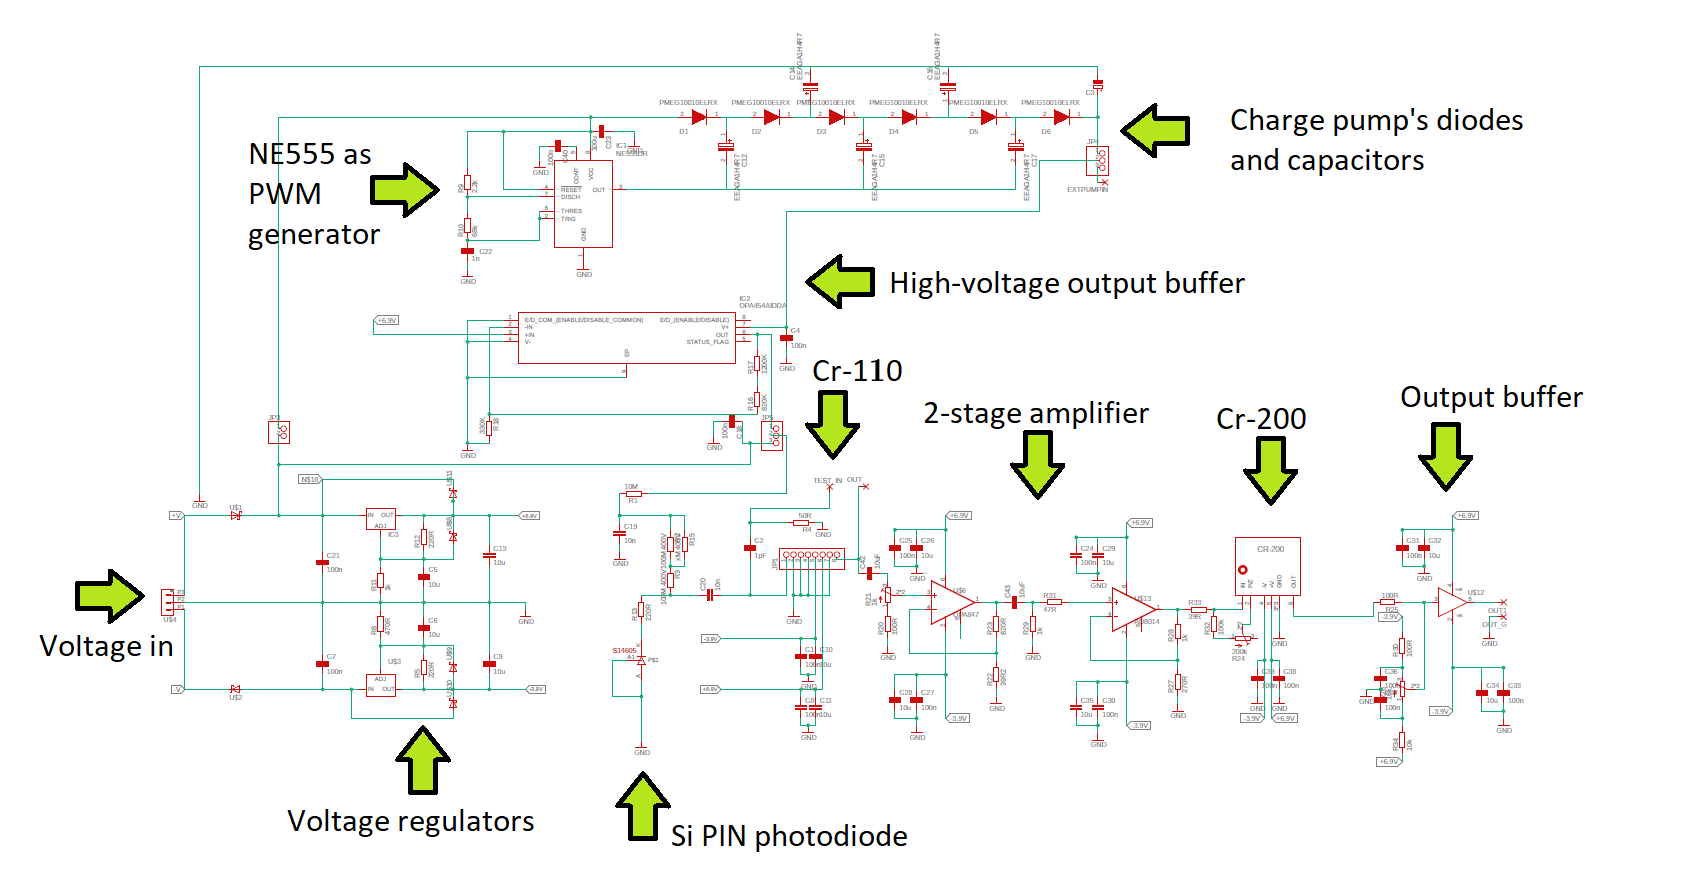
\includegraphics[scale=0.5, angle = 90]{./pictures/schemaPopis.png}
 \caption{Schematic of spectrometric chain PCB designed in EAGLE \cite{eagle}. Full schematic can be found in attachments.}
 \label{schematic}
 
\end{figure}

\newpage

\begin{figure}[H]
 \centering
 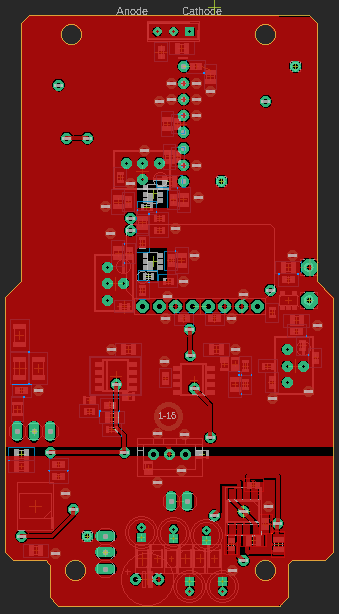
\includegraphics[scale=0.8, angle = 90]{./pictures/S14topLay.png}
 \caption{Layout of spectrometric chain PCB designed in EAGLE \cite{eagle}, top side layer.}
 \label{layout top}
 
\end{figure}

\begin{figure}[H]
 \centering
 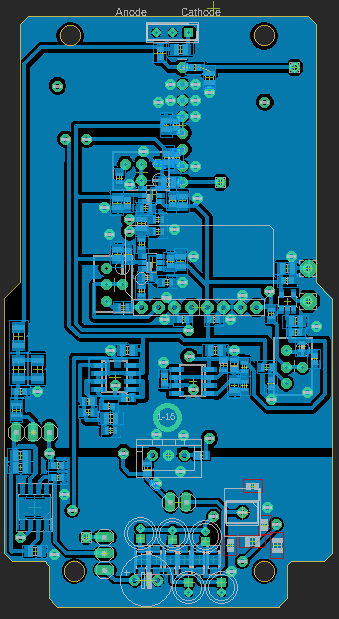
\includegraphics[scale=0.8, angle = 90]{./pictures/S14bottomLay.png}
 \caption{Layout of spectrometric chain PCB designed in EAGLE \cite{eagle}, bottom side layer.}
 \label{layout bottom}
 
\end{figure}
\newpage





\section{Grounding and Shielding}
To allow all the currents to have their return path with a sufficient conductivity, the main GND signal has to be spilled all around the circuit board. Even a small resistances in these paths may cause additional noise in signals. Currents from non-signal parts such as charge pump should have their return path different from the path of signal parts, and thus the spilled GND has to be cut to several separate parts connected together only at input voltage connector. This kind of layout is reffered as a star ground structure \cite{star}.

\par
The shielding box has to be connected to GND in carefully selected place to prevent the induced currents from shielding to flow over the signal ground of the detector. The best place to connect the shielding box with GND is near the input voltage connector.


\section{Photodiode input and preamplifier}
The photodiode is situated inside the box, and the cathode is connected to bias voltage and to preamplifier (CR-110) by capacitive coupling (10 nF capacitor). CR-110 application note also mentions an optional 220 $\Omega$ resistor connected before coupling capacitor to prevent CR-110 breakdown by large current spikes. Our experiences show that this resistor should not be omitted.

\par
The signal route has to be as short as possible. The layout should also be designed in ways to reduce the parasitic capacitances at the preamplifier input - the cooper connected to ground (GND) should be removed from areas around the signal input route and around input bias voltage route. 

\section{Amplification}
The preamplifier output is routed over capacitive coupling (to eliminate unwanted offset) and over potentiometer divider (to adjust signal amplitude) to the amplification stages. 

First amplification is achieved by two non-inverting amplifiers with OPA847 opamps. Each stage has the amplification of 32$\times$ (or less, this is different for every of our prototypes). Additional amplification 10$\times$ is done by shaper module CR-220. The OPA847 opamp datasheet \cite{OPA847} describes that these fast opamps are prone to unwanted oscillations, and therefore the GND around the opamp must be removed from both sides of the PCB. The output of shaper module is routed directly to output buffer opamp Max4201. The end of chain is buffered and connected to the output SMA connector mounted onto the aluminium box.


\section{Voltage supply}
The regulation of power supply (usually +15 V and -15 V) is done by LM317 and LM337 regulators, which convert input supply voltages into +7 V and -4 V. The output voltage of regulators is set by two resistors. However, these regulators produce heat, which negatively affects the SNR, so this heat has to be taken out of the circuit board by the thermal bridge connection to the aluminium box. To stabilize the temperature during the long runs, the shielding case has two additional peltier couples with fan attached onto it.

\par
S14605 requires bias voltage around +50 V, which can be supplied by 3-stage charge pump, assembled simply from capacitors, diodes and PWM generator - for example NE555. The charge pump is theoretically designed to multiply the the input voltage +15 V to +60 V. However, due to the fact that the rectifying diodes have some dropout and also   because the charge pump is not a stiff voltage source (even a small currents cause large dropout), the real bias voltage is around +50 V. The pump's output has to be filtered, because it can contain voltage spikes from switching frequency (NE555's frequency is set to 10 kHz). To filter this high voltage output the high-voltage opamp OPA454 is connected as buffer - the pump's voltage is connected as opamp supply, and the voltage from regulator (+7 V) is connected into opamp negative input pin. There is also a jumper which allows to switch between +15 V (for BPW34 photodiode) and +50 V.



\chapter{$^{57}$Co spectra measurement with integrated amplifier} 

To properly test the assembled PCB with attached S14605 photodiode (further referred as Si PIN detector) and to compare its detection efficiency for 14.4 keV photons with the detection efficiency of the other types of detectors - scintillator and gaseous detectors, the measurement setup with carefully designed geometry was constructed.

%\par
%
%The goal is to compare the Si PIN detector's detection efficiency of 14.4 keV photons with the detection efficiency of the other detectors - the scintillator and gaseous detectors.

\par

The onboard amplification is set in a way to have 14.4 keV energy peak in the second half of the channel range, which on the other hand result into the saturation of the higher energies, but the detection of these energies is not our focus.



\section{Measurement setup}
The measurement setup mainly consist of 3D printed parts - plastic holders for every detector and holders for radiation filters. All the holders have to be modular and easily interchangeable to allow the geometry to be kept same for every detector.
$^{57}$Co 2020 source is mounted onto the transducer (switched off in this measurement). Due to the fact, that the detectors have a different size of detection area, the irradiation has to be done through a collimator. To compare detection efficiency of the defined detection surface, the detector is irradiated through a hole ($d = 4$ mm) in a lead shielding, which works as collimator for $^{57}$Co source.

\par
For every detector, the sequence of five measurement was performed - without filter, with three filters and without a source. The relative detection efficiency for 14.4 keV is determined by Gaussian fit of the 14.4 keV peak in spectra with subtracted background. Every measurement of spectra ran 1200 s of live time.


\begin{figure}[H]
 \centering
 
\includegraphics[scale=0.8, angle = 90]{./pictures/NoPicture.jpg}
 \caption{Measurement setup.}
 \label{meas setup}
 
\end{figure}

\section{Si PIN detector measurement}

The output SMA connector is connected directly to the ORTEC MCA.
Three filters were placed before lead collimator - Cu (255 $\mu$m), Al (780 $\mu$m), Pb (5 mm).

\begin{figure}[H]
 \centering
 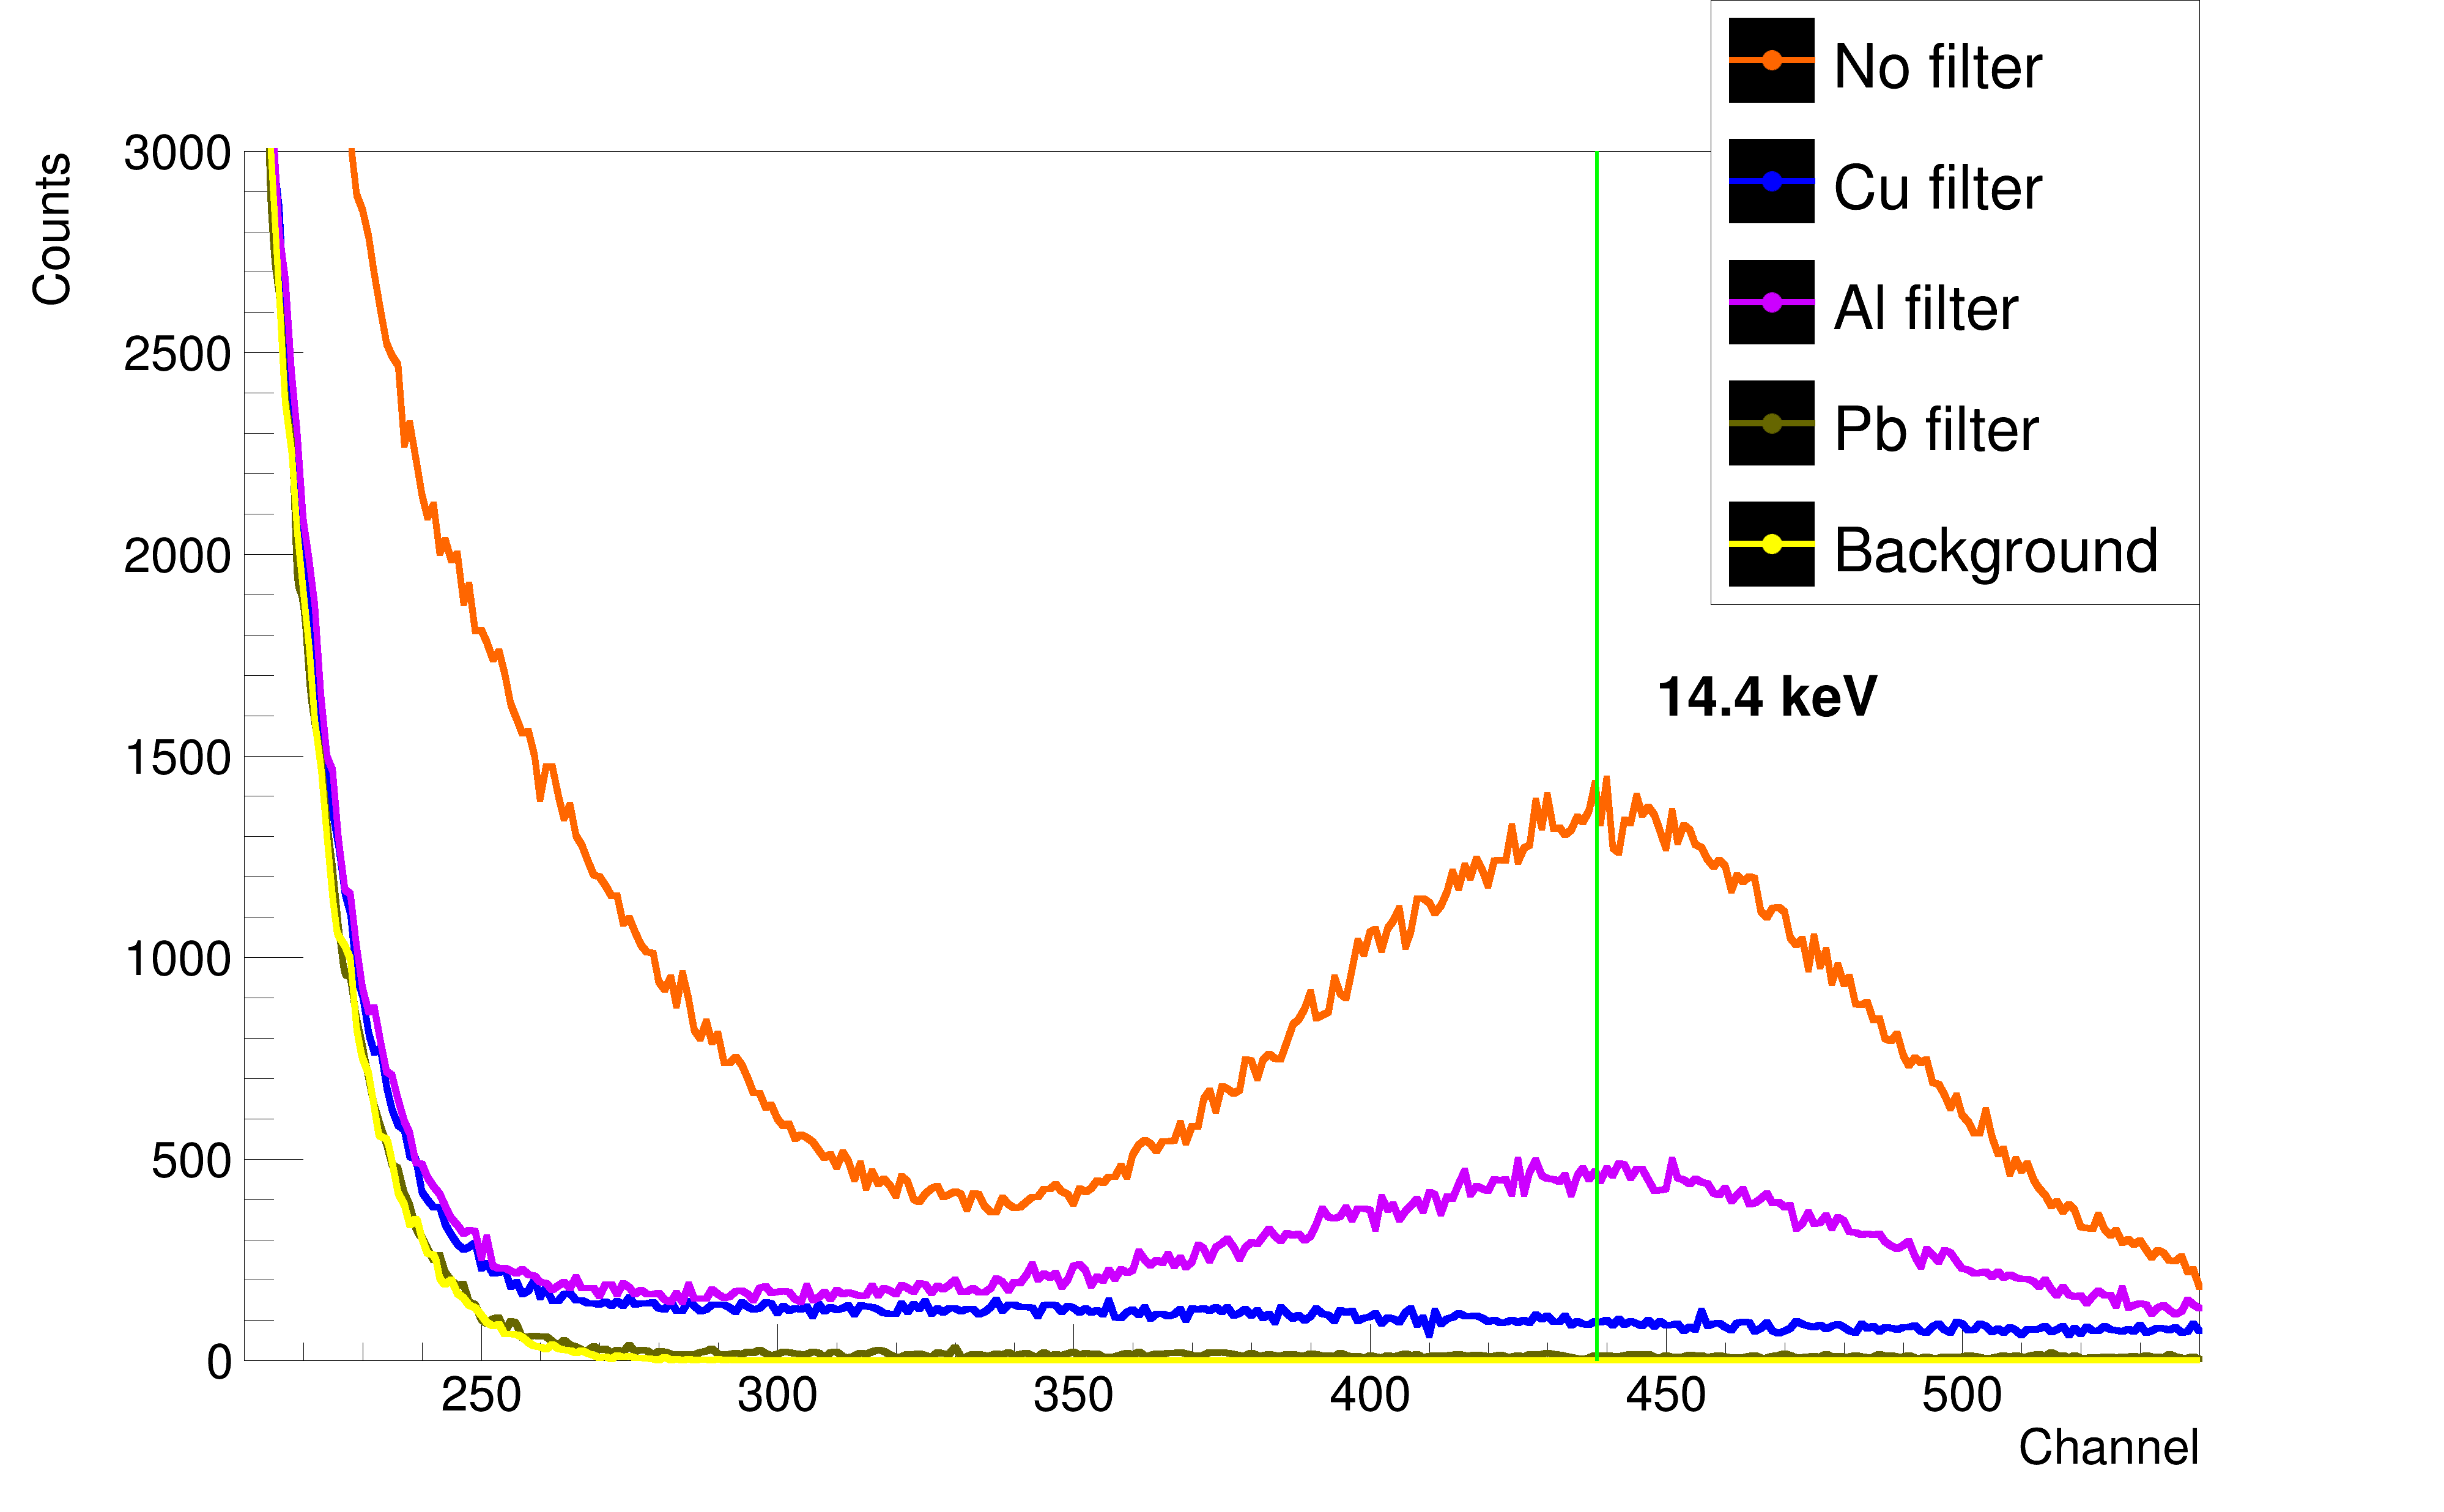
\includegraphics[scale=0.125, angle = 0]{./pictures/SemiSpectre.png}
 \caption{Si PIN detector $^{57}$Co spectra.}
 \label{Si PIN detector spectra.}
\end{figure}


It can be seen, that the noise in spectrum is much lesser than in case of ORTEC setups. The part of 6.4 keV peak can be also seen. Various ways were performed in order to reduce noise - cooling by ice, improving the shielding etc. However, none of them resulted into 6.4 keV energy peak without noise. Main part of remaining noise probably arises from Si PIN diode capacity ($C_{\textrm{S14605}} \approx 25$ pF). This fact can be confirmed by using the same PCB with photodiode with smaller capacity (for example BPW34, $C_{\textrm{BPW34}} \approx 10$ pF). Spectra of BPW34 attached to the integrated amplifier can be seen in the Figure \ref{BPW34 integrated amplifier spectra.}.


\begin{figure}[H]
\centering

\includegraphics[scale=0.125, angle = 0]{./pictures/NoPicture.jpg}
\caption{Spectra of BPW34 attached to the integrated amplifier.}
\label{BPW34 integrated amplifier spectra.}

\end{figure}


\section{Scintillator and gaseous detector measurement}
To measure the scintillator and the gaseous detector relative efficiency the same setup was used. As a gaseous detector was used tube LND45479, optimized for the 14.4 keV detection with amplification electronics based also on Cremat modules. In case of scintillator detector, our choice was photomultiplier tube R6095 \cite{R6095} with C9028-01 socket \cite{C9028}. As a scintillator crystal was used 0.4 mm thick YAP(Ce) and the amplification is done by the custom made amplifier\cite{STEJSKAL2019thesis}.

\begin{figure}[H]
\centering
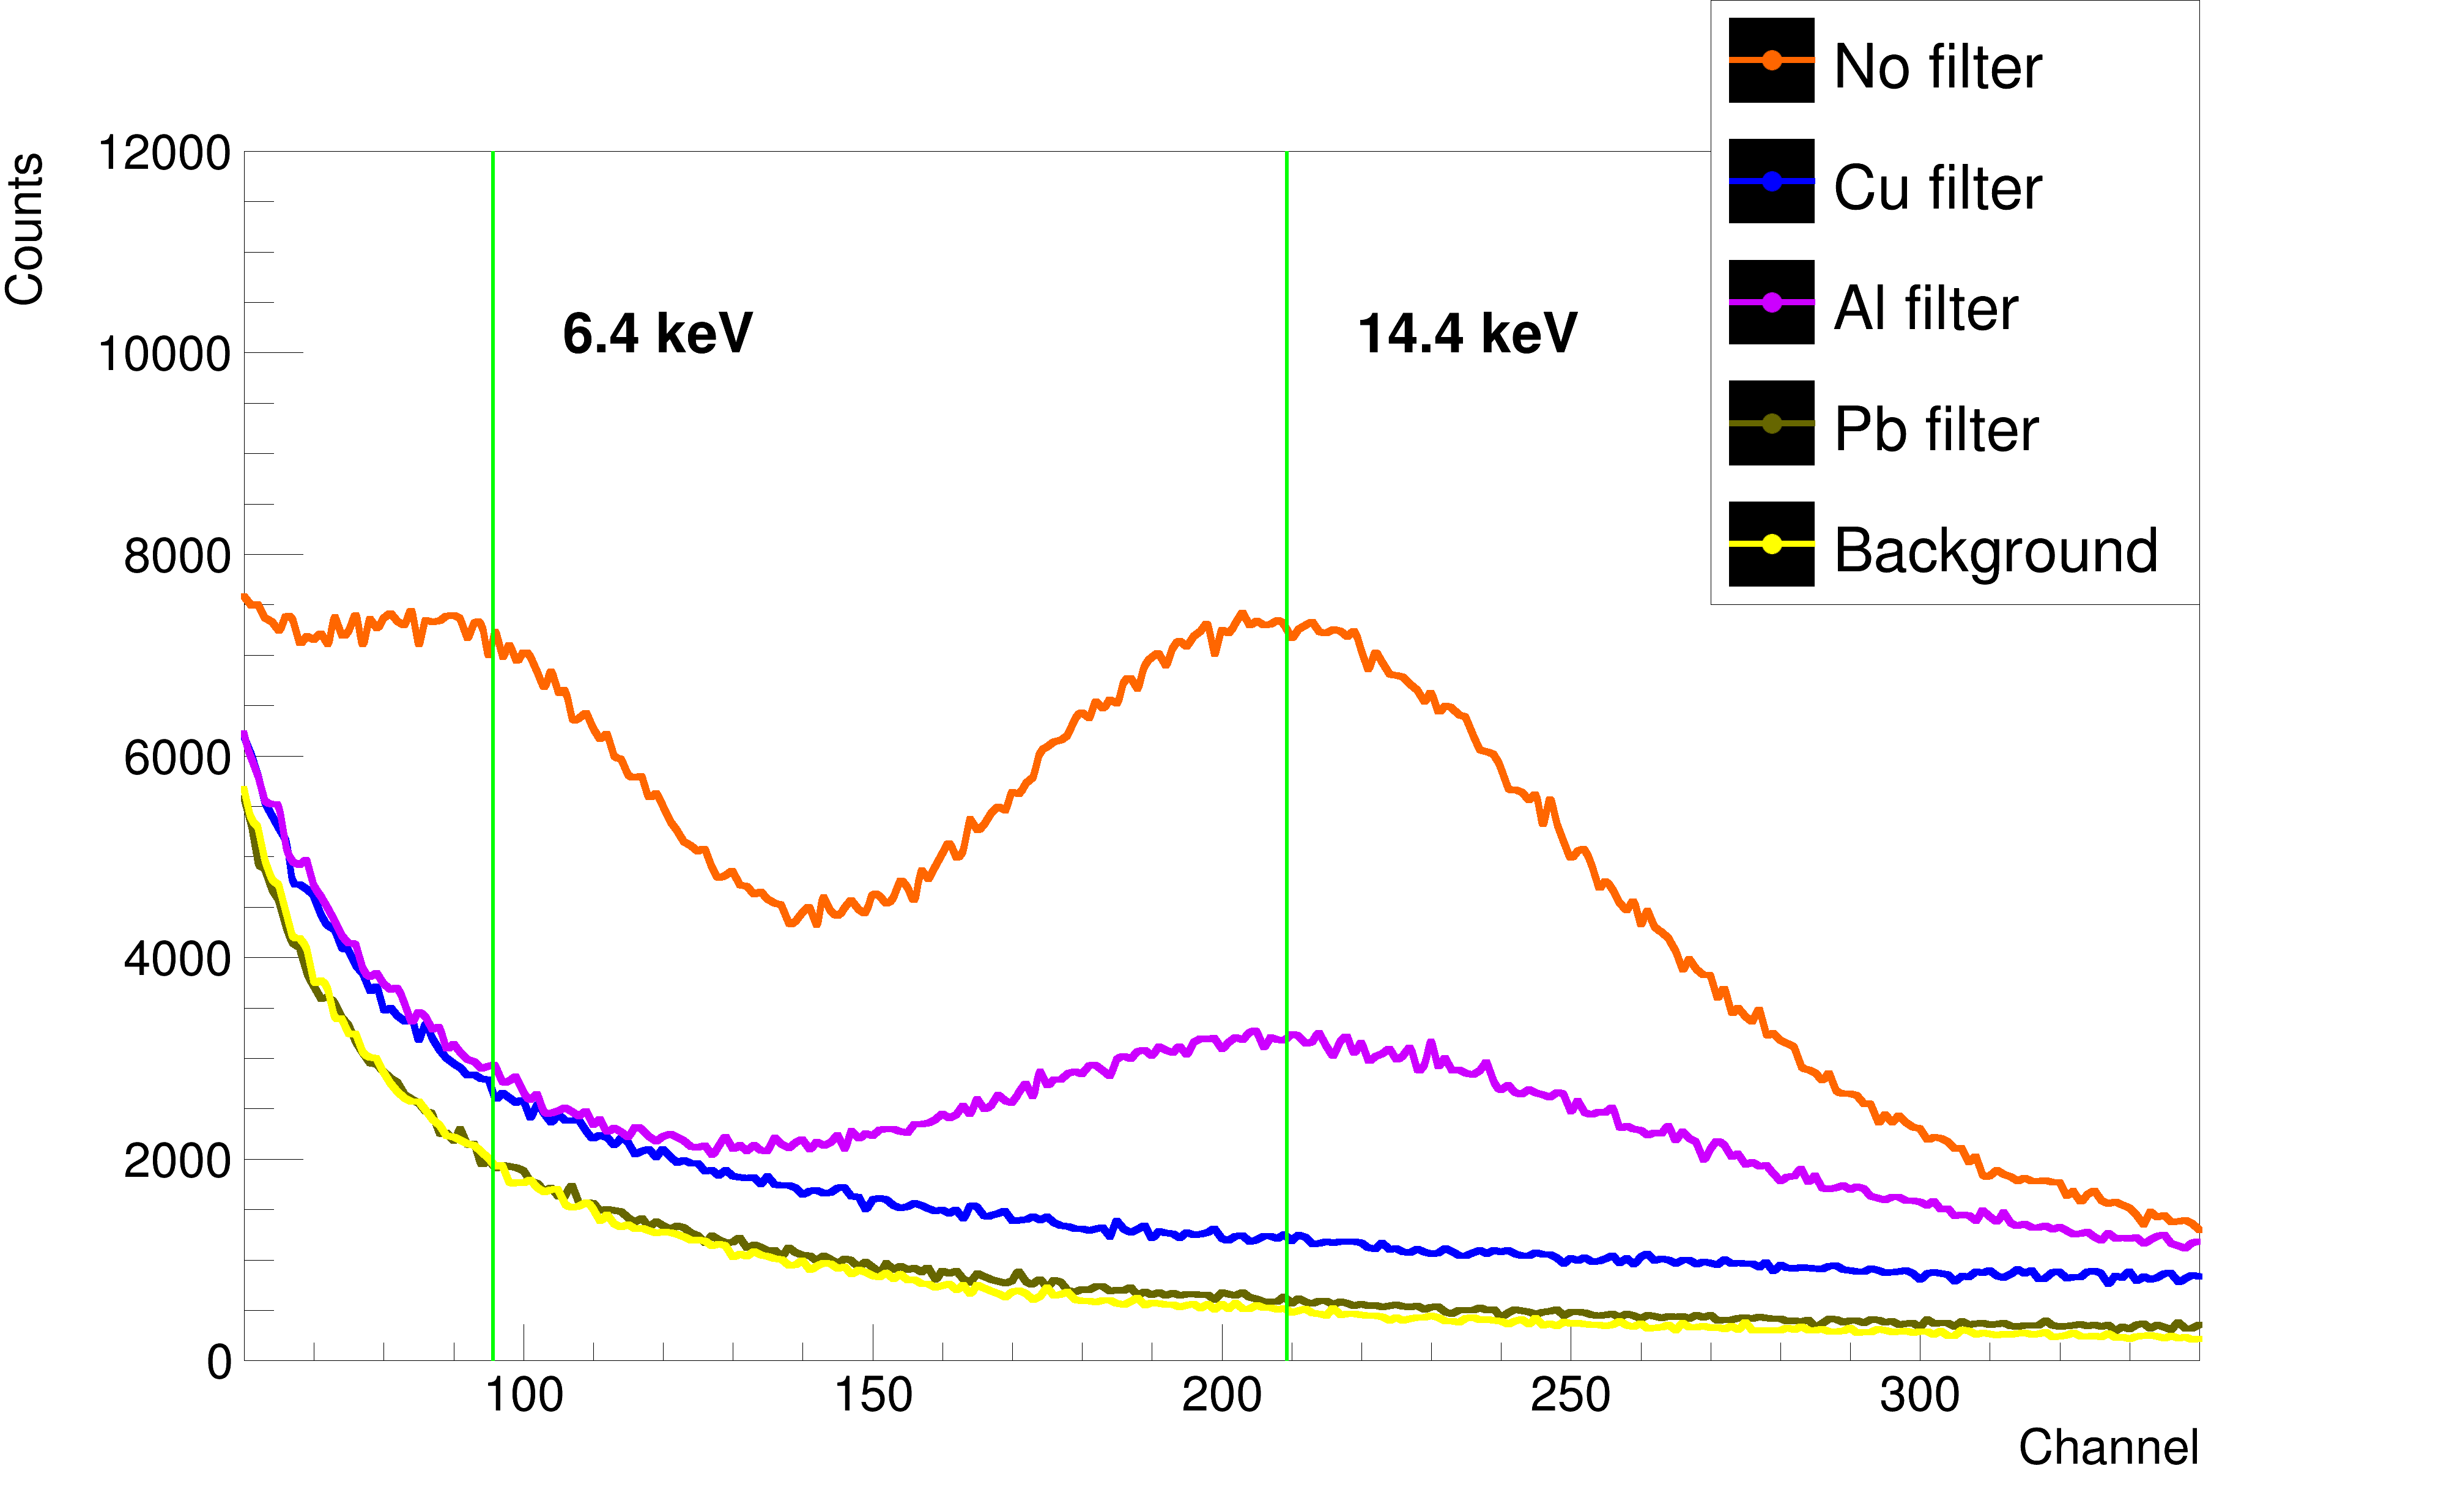
\includegraphics[scale=0.125, angle = 0]{./pictures/PMTSpectre.png}
\caption{Scintillator $^{57}$Co spectra.}
\label{Scintillator detector spectra.}
\end{figure}

\begin{figure}[H]
\centering
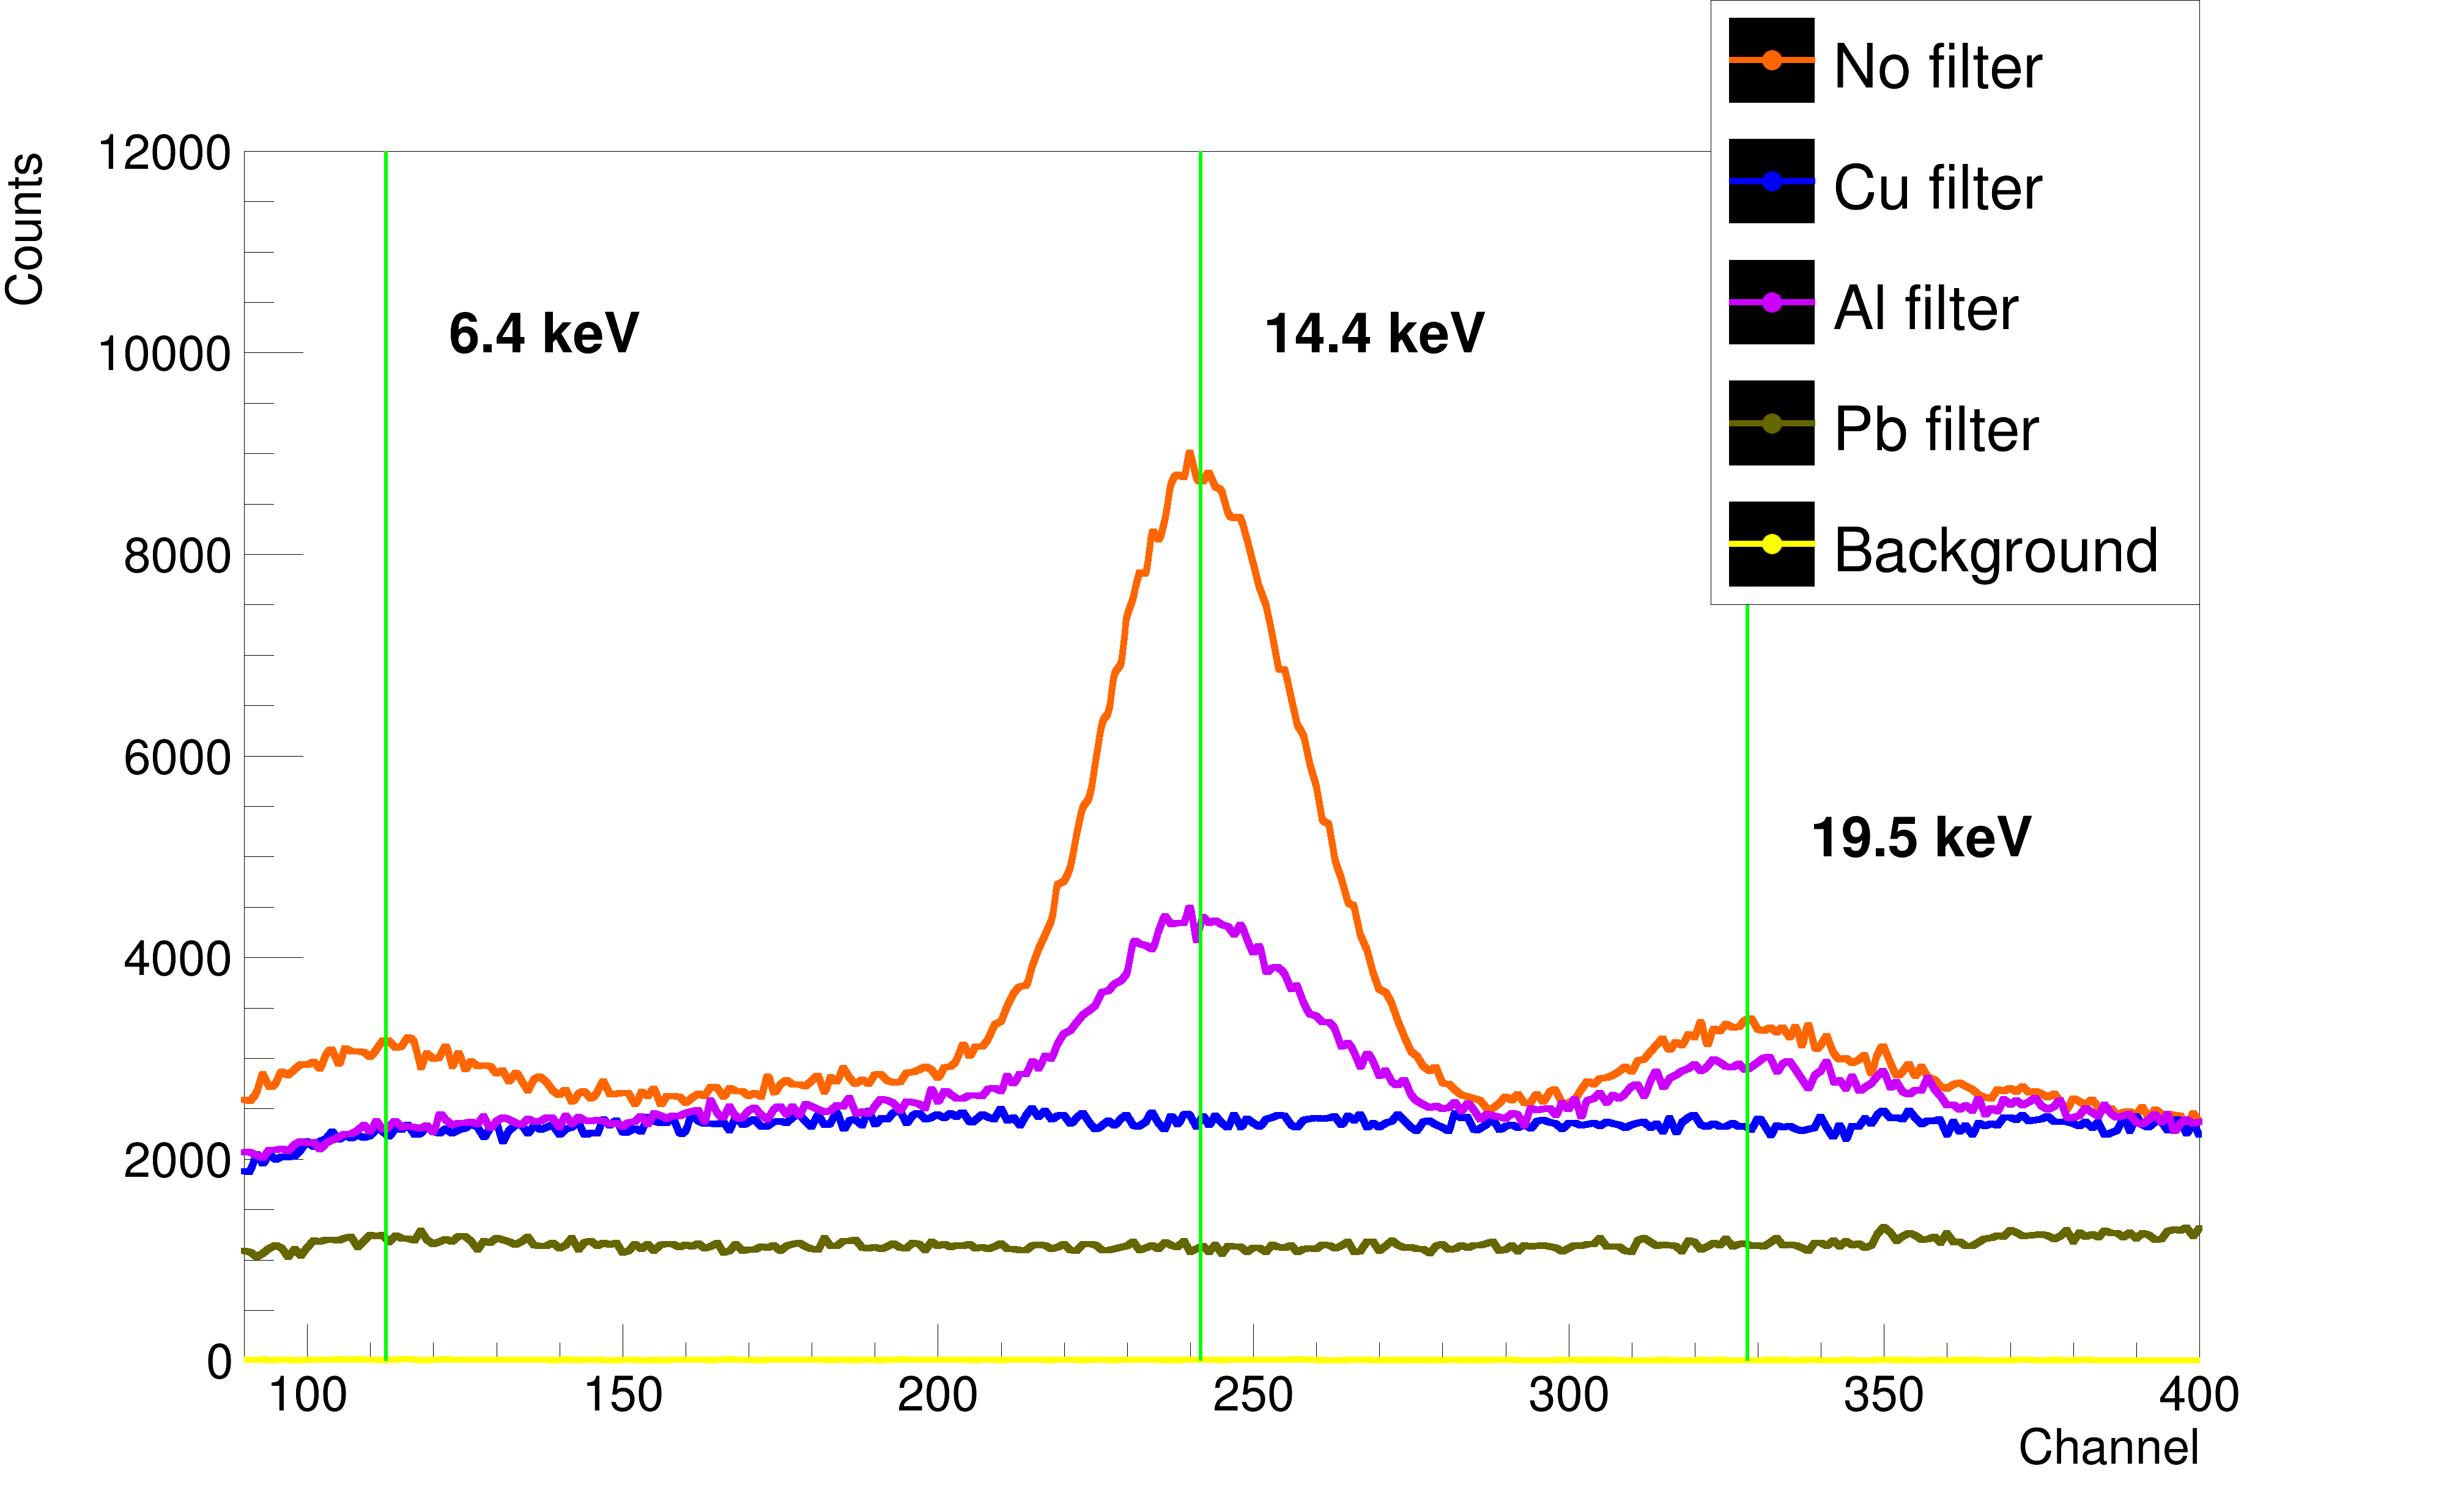
\includegraphics[scale=0.125, angle = 0]{./pictures/GasSpectre.png}
\caption{Gas $^{57}$Co spectra.}
\label{Gas detector spectra.}

\end{figure}


%In case of both detectors, both 14.4 keV and 6.4 keV peaks are fully observable. 
In spectra of gaseous detector, three narrow peaks can be observed - 14.4 keV peak and two small peaks - 6.4 keV and 19.5 keV. It also has a high level of Compton continuum.
The scintillator sees both 6.4 keV and 14.4 keV full energy peaks. However, its energy resolution is much worse - both peaks are noticeably wider and they overlap each other. 

\section{Results}
The sum of total counts for 14.4 keV and 6.4 keV full energy peaks along with the relative detection efficiency with respect to the most effective detector was calculated in the following way:

\begin{enumerate}
\item From the spectra without filter is subtracted the spectra with Cu filter. This provides a sufficient elimination of Compton continuum caused by 122 keV photons. 
\item The spectra obtained in previous step is fitted by a sum of Gaussians. Spectra of Si PIN and scintillator were fitted by sum of 2 Gaussians and in case of gas, the sum of 3 Gaussians is used.
\item The value of absolute counts (Gaussian's area) for the given energy spectra is calculated from the fit parameters with the uncertainties also taken from the fit.
\end{enumerate}




\begin{table}[H]
\centering
\begin{tabular}{|c|c|c|}
\hline
   & absolute & relative \\ \hline
Si PIN & $143000 \pm 3000$    & $0.291 \pm 0.008$  \\ \hline
gas & $231000 \pm 2000$    & $0.48 \pm  0.01$ \\ \hline
scintillator  & $491000 \pm 9000$    & $1$ \\ \hline
\end{tabular}
\caption{Table of calculated absolute and relative counts of 14.4 keV photons for each detector.}
 \label{144kevEFF}
\end{table}


The peak of 6.4 keV photons is not fully observable in the case of Si PIN detector. However, a rough estimation can be calculated using parameters obtained from Gaussian fit of partial 6.4 keV peak. Results in table \ref{64kevEFF} are considered to be only indicative. Note also that the setup wasn't designed to detect 6.4 keV photons - some detectors have slices of Al coating in detector window (Si PIN - ,scintillator - ,gas - window made of unknown metal).  

\begin{table}[H]
\centering
\begin{tabular}{|c|c|c|}
\hline
   & absolute & relative \\ \hline
Si PIN & $273000 \pm 8000$    & $1$  \\ \hline
gas & $20000 \pm 4000$    & $0.07 \pm 0.02$ \\ \hline
scintillator  & $184000 \pm 5000$    & $0.68 \pm 0.03$ \\ \hline
\end{tabular}
\caption{Table of calculated absolute and relative counts of 6.4 keV photons for each detector.}
 \label{64kevEFF}
\end{table}


\par
The results in table \ref{144kevEFF} show that the scintillator detector is the best detector for 14.4 keV photon among the three detectors that were tested. The Si PIN detector does not excel in detection of these energies and can be classified as the worst of the three. However, by the information provided by S14605 datasheet \cite{datS14605}, we come to a conclusion that the efficiency at 6.4 keV energies can be about 51 $\%$ better. This can be partially confirmed by rough estimations in table \ref{64kevEFF}, which describe the Si PIN as the best detector for 6.4 keV photons. To measure the full peak of 6.4 keV photons with S14605 photodiode, upgrades in electronics have to be made in order to increase the SNR, mainly the preamplifier has to be optimized for S14605's capacitance.





\chapter{Mössbauer spectra measurement}






% -----------------------------------------------
% Závěr
% -----------------------------------------------
\chapter*{Conclusion}
\addcontentsline{toc}{chapter}{Conclusion}

The first tests of Si PIN photodiodes were performed on setup consisting of ORTEC modular parts. All the three selected photodiodes (S14605, BPW34 and OPF430) produced spectrometric pulses and the gamma spectra of $^{57}$Co were successfully measured and interpreted. Characteristic full energy peaks of $^{57}$Co (14.4 keV, 122.1 keV and 136.5 keV) were observed as well as expected Compton continuum originating from Compton scattering of 122.1 keV inside the detector. It was found out, that the electromagnetic shielding plays a very important role in noise reduction. The Si PIN  photodiodes attached to charge preamplifier can not work properly without sufficient shielding. Cooling the photodiode also had an effect, but its significance was much lower.
\par
It was proven, that even a cheap Si PIN photodiode (BPW34 and OPF430) originally intended for detection of light can be employed as detector for gamma spectroscopy. However, it was shown that their detection efficiency is much worse than the detection efficiency of photodiode S14605, which is classified as x-ray detector.
\par
The front-end analog electronics for Si PIN detectors in form of PCB consisting of Cremat modules and SMD parts was successfully developed. This designed PCB placed into the shielding box integrates a significant part of spectrometric chain inside itself - PIN photodiode, the charge preamplifier, two amplification stages, the shaper and the high voltage supply for photodiode in form of a charge pump. For its functionality it requires only +15 V and -15 V power supply. Its output can be directly routed to the MCA. This Si PIN detector with integrated amplifier Int a full observation of 14.4 keV energy peak. The MS measurement setup employing constructed Si PIN detector was successfully assembled and the transmission MS spectra of a singlet sample was successfully measured.
\par
Two types of measurements were performed in order to compare the Si PIN detector with gaseous and scintillator detector - the measurement of 14.4 keV realative detection efficiency and the MS measurement. The only parameter of the Si PIN detector, which can be characterized as the best among the tested detectors is $E_{\textrm{MS}}$.

\par 
The development of PIN detector for transmission MS spectroscopy can continue by employing the photodiodes with better detection efficiency - by using Si photodiode with greater thickness or by using a photodiode made of a different material with higher $Z$ (for example Ge). To fully observe 6.4 keV energy peak, it will be necessary to employ a photodiode with lesser capacitance (greater thickness also implies lesser capacitance) or a preamplifier with a better characteristics. The development can also go on by the mathematical modelling of a better semiconductor detector for MS and by a theoretical simulations of its detection efficiency by using some of well-known programs for the simulation of passage of particles through matter such as the Geant4 \cite{Geant4}.

\par
The work on thesis was both very hard and experiencing, and thus it can be compared to have to chug a bottle of 50$\%$ vodka - get sick, get experienced.



% -----------------------------------------------
% Literatura a prameny
% -----------------------------------------------
%\begin{thebibliography}{99}
%\bibliographystyle{unsrt}
%\nocite{*}
%\bibliography{citations}
%\nocite{MALACARI2020102430}
\nocite{*}
%\nocite{Tomankova2016_1000061954}
%\nocite{VACULA2021167169}
%\addcontentsline{toc}{chapter}{Literatura}
%\bibitem{gravitation} MISNER, Ch. W.; THORNE, K. S.; WHEELER, J. A. %\emph{Gravitation}. San Francisco: W. Freeman, 1973.
%\end{thebibliography}
\printbibliography[notcategory=skipbibliography]
%\newpage
%\chapter*{Attachment: Measurement and analysis programs}
%Measurement folder - scripts for controlling measurement
%\newline
%PulseAnalysis folder - scripts for PMT pulse analysis
%\newline
%FASTanalyze.cpp - calibration data analysis
%\newline
%main.c - Nucleo F446RE's synchronized sampling and PID regulator firmware
\end{document}
% Konec souboru %%%%%%%%%%%%%%%%%%%%%%%%%%%%%%%%%%%%%%%%%%%%%%%%%%%%%%%%%%%%
